\documentclass{scrreprt}
\usepackage{standalone}
\usepackage{caption}
\usepackage{subcaption}
\usepackage{graphbox} % 1120
\usepackage{chez}

\usepackage{eighteen905}
\usetikzlibrary{decorations.pathmorphing,
                decorations.markings,
                fadings}

\graphicspath{{figures/}}

\title{18.905 Notes}
\author{Jason Chen \\ Lecturer: Jeremy Hahn}
\date{Last Updated: \today}

\begin{document}
\maketitle
\setcounter{tocdepth}{2}
\tableofcontents

\documentclass{standalone}
\usepackage{chez}

\begin{document}
\chapter{September 02, 2020}
The first half of the course is on \vocab{homology}, where we want to study
space by asking how many ``holes'' a space has.

For example, a circle, the letter Y, and a line segment with
three circles attached to it have \(1\), \(0\), and \(3\) holes respectively.
\begin{center}
  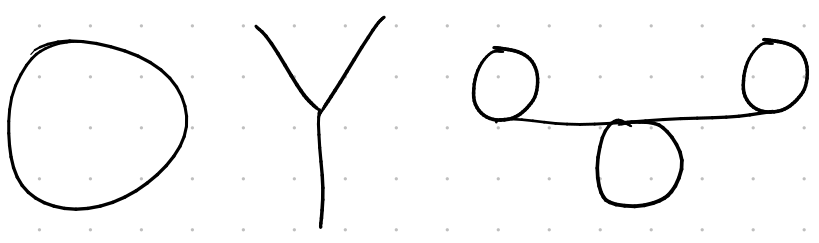
\includegraphics[width=0.5\textwidth]{18_905-200902-1.png}
\end{center}
The fundamental group is one way of measuring the number of holes, but we will
present a different way of understanding the number of holes in these spaces
with the first homology group \(H_1\).

Let's first provide an algorithm of how to find the homology of a space.
\begin{example}[Homology of the circle]
  First, we transform the space into a more graph-theoretic structure
  by adding some vertices, and then making the edges directed, like so:
  \begin{center}
    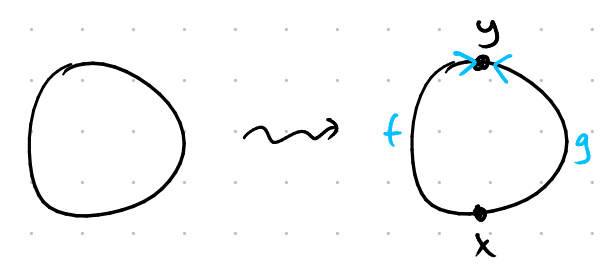
\includegraphics[width=0.5\textwidth]{18_905-200902-2.png}
  \end{center}
  Let \(\ZZ\{f, g\}\) denote the free abelian group generated by
  \(f\) and \(g\). Consider the group homomorphism
  \begin{align*}
    \partial \colon &\ZZ\{f, g\} \to \ZZ\{x, y\} \\
      & f \mapsto y - x \\
      & g \mapsto y - x,
  \end{align*}
  where we mapped each edge to their ``target minus source''. Note that
  the kernel of \(\partial\) is the integer multiples of \(f - g\).
  In particular, \(\ker \partial\) is generated by \emph{one} element,
  so there is \emph{one} hole.
  This kernel is called the first homology group \(H_1\) of the circle.
\end{example}

\begin{example}[Homology of the letter Y]
  Again, transform the space into a combinatorial gadget by assigning
  vertices and directing edges:
  \begin{center}
    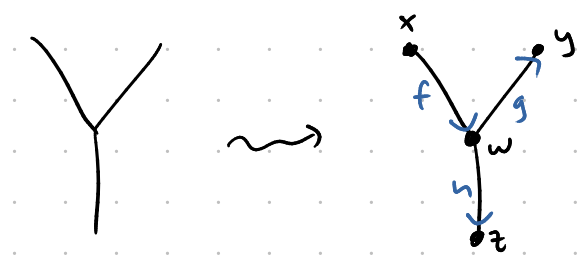
\includegraphics[width=0.5\textwidth]{18_905-200902-3.png}
  \end{center}
  We consider the homomorphism
  \begin{align*}
    \partial \colon & \ZZ\{f, g, h\} \to \ZZ\{x, y, z, w\} \\
      & f \mapsto w - x \\
      & g \mapsto y - w \\
      & h \mapsto z - w.
  \end{align*}
  The only element that gets sent to \(0\) by \(\partial\) is \(0\),
  so \(\ker \partial\) is the free abelian group on \(\nullset\).
  Therefore, there are no holes.
\end{example}

The kernel we have been computing is the first homology group,
and the number of generators corresponds to the number of holes.

This algorithm involves many arbitrary decisions.
  Why is it giving the same answer each time?
  How does this generalize to larger dimensional spaces?

\end{document}

\documentclass{standalone}
\usepackage{chez}

\begin{document}
\chapter{September 04, 2020}
Last time, we computed the homology group of a combinatorial object,
a directed graph. However, there are two problems that arise:
\begin{enumerate}
  \item We want to handle higher dimensional objects.
  \item We want to handle topological spaces and
  not just combinatorial objects.
\end{enumerate}

Let's try to work on the first issue.
\begin{definition}
  A \vocab{semisimplicial set} \(X\) is
    a sequence of sets \(X_0, X_1, X_2, \dots\) and
    functions
    \begin{align*}
      d_0, d_1 &\colon X_1 \to X_0 \\
      d_0, d_1, d_2 &\colon X_2 \to X_1 \\
      &\shortvdotswithin{\colon}
      d_0, d_1, d_2, \dots, d_n &\colon X_n \to X_{n-1} \\
      \MTFlushSpaceAbove
      &\vdotswithin{\colon}
    \end{align*}
  that satisfy the \vocab{simplicial identities}
  \[
    d_i d_j = d_{j - 1} d_i \quad
    \text{whenever \(i < j\)}.
  \]

  These sets \(X_n\) are called the \vocab{\(n\)-simplices}, and the maps
  \(d_i\) are called the \vocab{face maps}.
\end{definition}

\begin{example}
  A semisimplicial set with \(\nullset = X_2 = X_3 = \cdots\), etc.\
  is just a directed graph
  \begin{align*}
    X_0 &= \set{\text{vertices}} \\
    X_1 &= \set{\text{edges}}
  \end{align*}
  with
  \[
    d_0, d_1 \colon X_1 \to X_0,
  \]
  with \(d_0\) mapping an edge to the ``target''
  and \(d_1\) mapping an edge to the ``source''.
\end{example}

\begin{example}
  If we have the following combinatorial structure:
  \begin{center}
    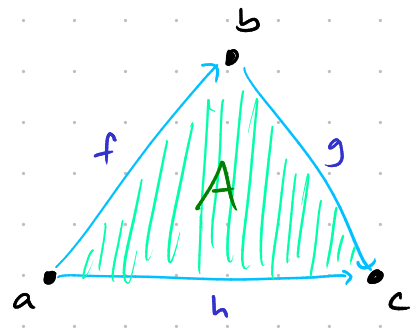
\includegraphics[width=0.3\textwidth]{18_905-200904-2.png} % chktex 8
  \end{center}
  This represents the semisimplicial set with
  \begin{align*}
    X_0 &= \set{a, b, c} \\
    X_1 &= \set{f, g, h} \\
    X_2 &= \set{A} \\
    X_3 = X_4 &= \nullset. \\
    \MTFlushSpaceAbove
    &\vdotswithin{=}
  \end{align*}
  Then we have the functions
  \[
    d_0, d_1 \colon X_1 \to X_0
    \qquad \text{and} \qquad
    d_0, d_1, d_2 \colon X_2 \to X_1
  \]
  where
  \begin{align*}
    d_0 f &= b &
      d_1 f &= a &
      d_0 A &= g \\
    d_0 g &= c &
      d_1 g &= b &
      d_1 A &= h \\
    d_0 h &= c &
      d_1 h &= a &
      d_2 A &= f.
  \end{align*}
  To see why \(d_0, d_1, d_2\) act on \(A\) the way they do,
  note that the simplicial identities require
  \[
    d_0 d_2 A = d_1 d_0 A.
  \]
  The element in \(X_0\) that must equal these two values must be a source
  and a target, so it must be \(b\). The values of \(d_0 A\), \(d_1 A\),
  and \(d_2 A\) follow.
\end{example}

Note that it's important that the edges go forward from \(a \to b \to c\)
and backwards from \(c \gets a\). Otherwise, the simplicial identity would
not be able to uniquely define \(d_0, d_1, d_2\) on \(A\).

\section{Homology}
If \(X\) is a semisimplicial set, then let \(S_n(X)\) be the abelian group
of \vocab{singular \(n\)-chains},
the free abelian group generated by the set \(X_n\) of \(n\)-simplices.

\begin{definition}
  For \(n \geq 1\), the \vocab{boundary operators} are group homomorphisms
  \[
    \partial_n \colon S_n(X) \to S_{n - 1}(X)
  \]
  defined by the generators \(\sigma \in X_n\) where
  \[
    \sigma \mapsto \sum_{k = 0}^{n} (-1)^k d_k \sigma.
  \]

  We also define \(\partial_0 \colon S_0(X) \to 0\) to be
  the zero homomorphism.
\end{definition}

\begin{definition}
  Suppose \(X\) is a semisimplicial set. The group of \vocab{\(n\)-cycles}
  in \(X\), denoted by \(Z_n(X)\) is the kernel of \(\partial_n\).
  
  The group of \vocab{\(n\)-boundaries} in \(X\), denoted \(B_n(X)\),
  is the image of \(\partial_{n+1}\).
\end{definition}

\begin{exercise}[On homework]
  \(B_n(X)\) is a subgroup of \(Z_n(X)\), which is in turn
  a subgroup of \(S_n(X)\).
\end{exercise}

We can therefore define the \vocab{\(n\)th singular homology group} of \(X\),
\[
  H_n(X) = Z_n(X) / B_n(X) = \frac{\ker \partial_n}{\img \partial_{n+1}},
\]
which is an abelian group because the quotient of an abelian group is abelian.
This intuitively measures the number of \(n\)-dimensional holes in \(X\).

% % % % % % % % % % % % % % % % % % % % % % % % % % % % % % % % % % % % % % % %
\section{Topological spaces}
\begin{question}
  How do we get a semisimplicial set out of a topological space?
\end{question}

The basic tool we will use are simplices.
\begin{definition}
  For \(n \geq 0\), the \vocab{standard \(n\)-simplex} \(\Delta^n\) is
  the subspace of \(\RR^{n+1}\) that is the convex hull of the standard basis
  \(\set{e_0, \dots, e_n}\) in \(\RR^{n+1}\). In particular,
  \[
    \Delta^n = \set*{\sum t_i e_i \mid \sum t_i = 1, t_i \geq 0}
      \subseteq \RR^{n+1}.
  \]
  The \(t_i\) are sometimes called \vocab{barycentric coordinates}.
\end{definition}

\begin{example}
  \(\Delta^1 \subseteq \RR^2\) is
  the line segment from \((1, 0)\) to \((0, 2)\).

  \(\Delta^2 \subseteq \RR^3\) is
  the triangle with vertices \(\set{(1, 0, 0), (0, 1, 0), (0, 0, 1)}\).
\end{example}

\begin{definition}
  For a topological space \(X\), a \vocab{singular \(n\)-simplex in \(X\)}
  is a continuous map \(\sigma \colon \Delta^n \to X\).
  We will often drop the adjective ``singular''.
  Let \(\Sing_n(X)\) be the set of all \(n\)-simplices in \(X\).
\end{definition}

We can assemble these into a semisimplicial set.
In particular, there are maps \(d_i \colon \Sing_n(X) \to \Sing_{n-1}(X)\)
that come from ``forgetting'' the basis element \(e_i\).
In particular, we have the function \(d_1 \colon \Delta^2 \to \Delta^1\)
that takes the segment (\(\Delta^1\)) that does not include
the vertex corresponding to \(1\).
So given \(\sigma \colon \Delta^2 \to X \in \Sing_2(X)\),
we can restrict \(\sigma\) to \(d_1 \Delta^2 = \Delta^1\),
giving a map \(\Delta^1 \to X \in \Sing_1(X)\).
\begin{align*}
  d_1 \colon& \Sing_2(X) \to \Sing_1(X) \\
    & \sigma \to \sigma\mathord\vert_{d_1 \Delta^2}
\end{align*}
Therefore, \(\Sing(X)\), the collection of all of the \(\Sing_n\) sets,
is a semisimplicial set.

\begin{remark}
  For more intuition, look at Hatcher's treatment of \(\Delta\)-complexes
  (another name for semisimplicial set).
\end{remark}

\begin{definition}
  If \(X\) is a topological space, we can define
  \begin{align*}
    S_n(X) &= S_n(\Sing X), &
    Z_n(X) &= Z_n(\Sing X), &
    B_n(X) &= B_n(\Sing X), \qquad \text{and} &
    H_n(X) &= H_n(\Sing X).
  \end{align*}
\end{definition}

Overall, we are transforming geometric objects into combinatorial objects,
and then in turn transforming them into algebraic objects so that they are
easier to study.
\[
  \begin{tikzcd}
    \parbox[t]{2.8cm}{\centering Topological spaces (geometric)}
      \arrow[r, "\Sing"] &
    \parbox[t]{3cm}{\centering Semisimplicial sets (combinatorial)}
      \arrow[r, "H_n"] &
    \parbox[t]{2.5cm}{\centering Abelian groups (algebraic)}
  \end{tikzcd}
\]


\end{document}

\documentclass{standalone}
\usepackage{chez}

\begin{document}
\chapter{September 09, 2020}
Note that if \(X \to Y\) is a continuous map of topological spaces,
and \(\sigma \colon \Delta^n \to X\) is a continuous function,
then the composition of them \(\Delta^n \to X \to Y\) is also continuous.
Therefore, a map \(X \to Y\) induces a map \(\Sing_n(X) \to \Sing_n(Y)\).

\section{Category theory}
\begin{definition}
  A \vocab{category} \(\mathcal C\) consists of:
  \begin{itemize}[nosep]
    \item A class \(\Obj C\) of \vocab{objects} in \(\mathcal C\).
    \item For every pair of objects \(X, Y \in \Obj \mathcal C\),
      a set of \vocab{morphisms} \(\Hom_{\mathcal C}(X, Y)\).
    \item For every object \(X \in \Obj \mathcal C\),
      an identity morphism \(1_X \in \Hom_{\mathcal C}(X, X)\).
    \item For every triple of objects \(X, Y, Z \in \Obj \mathcal C\),
      a composition operation
      \[
        \Hom_{\mathcal C}(X, Y) \times \Hom_{\mathcal C}(Y, Z)
        \to
        \Hom_{\mathcal C}(X, Z)
      \]
      written \((f, g) \mapsto g \circ f\).
  \end{itemize}
  These data are required to satisfy two properties:
  \begin{itemize}[nosep]
    \item \(1_Y \circ f = f\) for all \(f \in \Hom_{\mathcal C}(X, Y)\) and
      \(f \circ 1_Y = f\) for all \(f \in \Hom_{\mathcal C}(Y, X)\).
    \item Composition is associative, i.e.
      \[
        (h \circ g) \circ f = h \circ (g \circ f)
      \]
      whenever these operations are defined.
  \end{itemize}
\end{definition}

Note that we say that \(\Obj C\) is a class instead of a set to prevent
logical paradoxes, such as talking about the set of all sets.
We can just think about these as sets, and our intuition would
work perfectly well.

\begin{example}
  \begin{itemize}[nosep]
    \item \(\cSet\) is the category of sets.
    \(\Obj(\cSet)\) is the class of all sets and morphisms are functions:
    if \(X, Y\) are two sets, then \(\Hom_{\cSet}(X, Y)\) is
    the set of all functions \(X \to Y\).

    \item \(\cAb\) is the category of abelian groups.
    \(\Hom_{\cAb}(A, B)\) refers to the set of all group homomorphisms
    \(A \to B\).

    \item \(\cat{Vect_\RR}\) is the category of real vector spaces.
    Morphisms are linear transformations.

    \item \(\cTop\) is the category of topological spaces.
    \(\Hom_{\cTop}(X, Y)\) is the set of continuous maps \(X \to Y\).
  \end{itemize}
\end{example}

A note on notation: If \(\mathcal C\) is a category, sometimes we say
\(X \in \mathcal C\) to mean \(X \in \Obj C\) and
\(f \colon X \to Y\) to mean \(f \in \Hom_{\mathcal C}(X, Y)\).
We also may sometimes say map instead of morphism.

\begin{definition}
  A morphism \(f \colon X \to Y\) in a category \(\mathcal C\) is called an
  \vocab{isomorphism} if there exists a map \(g \colon Y \to X\) such that
  \[
    g \circ f = 1_X, \qquad \text{and} \qquad f \circ g = 1_Y.
  \]
\end{definition}

\begin{example}
  A morphism in \(\cSet\) is an isomorphism if and only if
  it is a bijection.

  A morphism in \(\cAb\) is an isomorphism if and only if
  it is a group isomorphism.

  A morphism in \(\cTop\) is the same thing as a homeomorphism.
\end{example}

\begin{proposition}
  If \(f \colon X \to Y\) is an isomorphism in a category \(\mathcal C\),
  then the inverse \(g \colon Y \to X\) is unique.
\end{proposition}
\begin{proof}
  Suppose \(g, g' \colon Y \to X\) are two inverses of \(f \colon X \to Y\).
  Then
  \[
    g = g \circ 1_Y = g \circ (f \circ g') =
    (g \circ f) \circ g' = 1_X \circ g' = g'. \qedhere
  \]
\end{proof}

\begin{definition}
  Given categories \(\mathcal C, \mathcal D\), a \vocab{functor}
  \(F \colon \mathcal C \to \mathcal D\) consists of:
  \begin{itemize}[nosep]
    \item An assignment \(F \colon \Obj \mathcal C \to \Obj \mathcal D\), and
    \item for all \(X, Y \in \Obj \mathcal C\), a function
      \[
        F \colon \Hom_{\mathcal C}(X, Y) \to \Hom_{\mathcal D}(F(X), F(Y)).
      \]
  \end{itemize}
  These are required to satisfy the following two properties:
  \begin{itemize}[nosep]
    \item For all \(X \in \Obj \mathcal C\), \(F(1_X) = 1_{F(X)}\).
    \item For all composable pairs of morphisms \(f, g\) in \(\mathcal C\),
    \[
      F(g \circ f) = F(g) \circ F(f).
    \]
  \end{itemize}
\end{definition}

\begin{example}
  For each \(n \geq 0\), there are the functors
  \begin{align*}
    \Sing_n \colon& \cTop \to \cSet \\
      & X \to \set{\sigma \colon \Delta^n \to X} \\
    S_n \colon& \cTop \to \cat{Ab}.
  \end{align*}
\end{example}

There is a huge category \(\cCat\) of categories. In particular,
the objects of \(\cCat\) are categories, and the morphisms are functors.
Warning: If \(\mathcal C, \mathcal D\) are two categories, then
\(\Hom_{\cCat}(\mathcal C, \mathcal D)\) might be a class and not a set.
In particular, we can compose functors.

\begin{example}
  There is a functor
  \[
    \operatorname{Free} \colon \cSet \to \cat{Ab}
  \]
  that maps a set to the free abelian group generated by the set.
  In particular,
  \(S_n = \operatorname{Free} \circ \Sing_n \colon \cTop \to \cat{Ab}\).
\end{example}

If \(f \colon X \to Y\) is a map in \(\cTop\), then there is a diagram
for each \(0 \leq i \leq n\)
\[
  \begin{tikzcd}
    \Sing_n(X)\arrow[r, "d_i"]\arrow[d, "\Sing_n(f)", swap] &
      \Sing_{n-1}(X)\arrow[d, "\Sing_{n-1}(f)"] \\
    \Sing_n(Y)\arrow[r, "d_i"] & \Sing_{n-1}(Y)
  \end{tikzcd}
\]
that commutes. In category theory, one can generalize this kind of diagram.

\begin{definition}
  Let \(F, G \colon \mathcal C \to \mathcal D\) be two functors.
  A \vocab{natural transformation} \(\Theta \colon F \to G\) consists of
  maps \(\Theta_X \colon F(X) \to G(X)\) for each \(X \in \mathcal C\)
  such that for all \(f \colon X \to Y\), the following diagram commutes:
  \[
    \begin{tikzcd}
      F(X)\arrow[r, "\Theta_X"]\arrow[d, "F(f)", swap] &
        G(X)\arrow[d, "G(f)"] \\
      F(Y)\arrow[r, "\Theta_Y"] &
        G(Y)
    \end{tikzcd}
  \]
\end{definition}

\begin{example}
  Our previous example becomes the following:
  Suppose \(n \geq 1\) and \(0 \leq i \leq n\). Then there is
  a natural transformation
  \[
    d_i \colon \Sing_n \to \Sing_{n - 1},
  \]
  where \(\Sing_n, \Sing_{n-1}\) are functors \(\cTop \to \cSet\).
\end{example}

\begin{definition}
  A natural transformation \(\Theta \colon F \to G\) is called a
  \vocab{natural isomorphism} if each map \(\Theta_X\) is an isomorphism
  for all \(X \in \Obj \mathcal C\).
\end{definition}

Suppose \(\mathcal C, \mathcal D\) are categories and
\(\Obj \mathcal C\) is a set (as opposed to a class).
Then there is another category \(\cat{Fun}(\mathcal C, \mathcal D)\)
of functors where the morphisms are natural transformations of functors.
Note that if \(\Obj \mathcal C\) is not a set, then some sets of morphisms
would be a class instead of a set, while the definition requires a set.


\end{document}

\documentclass{standalone}
\usepackage{chez}

\begin{document}
\chapter{September 11, 2020}
Today we will finish putting semisimplicial sets into
a category theory viewpoint.

Suppose \(\mathcal C\) is a category. Then a new category we can consider is
the \vocab{opposite category} \(\mathcal C^{\mathrm{op}}\) with
\begin{itemize}[nosep]
  \item \(\Obj(\mathcal C^\op) = \Obj(\mathcal C)\)
  \item For \(X, Y \in \Obj(\mathcal C^\op)\),
  \(\Hom_{\mathcal C^\op}(X, Y) = \Hom_{\mathcal C}(Y, X)\).
\end{itemize}
In particular, if \(f \in \Hom_{\mathcal C}(Y, X)\), we use \(f^\op\)
to represent the corresponding object of \(\Hom_{\mathcal C^\op}(X, Y)\).
The composition law is
\[
  (f \circ g)^\op = g^\op \circ f^\op.
\]

A good way to think about the opposite category is through functors.
As a category itself, \(\mathcal C^\op\) is essentially the same as
\(\mathcal C\), but a functor \(F \colon \mathcal C^\op \to \mathcal D\)
can be thought of as a function that still takes objects in \(\mathcal C\)
to objects in \(\mathcal D\), but takes maps \(c \to c'\) in \(\mathcal C\)
to maps \(F(c') \to F(c)\) in \(\mathcal D\).


\begin{example}
  Recall the category \(\cat{Vect}_\RR\) of real vector spaces.
  Every vector space \(V\) has a dual
  \(V^* = \underline{\Hom}_{\cat{Vect}_\RR}(V, \RR)\),
  where the underline indicates that the \(\Hom\) is a vector space itself.

  Note that if \(f \colon W \to V\) is a linear map, then the corresponding
  map \(f^* \colon V^* \to W^*\) in the opposite category maps
  \[
    f^* \colon
    \underset{\mathclap{\in V^*}}{(g \colon V \to \RR)}
    \mapsto
    \underset{\mathclap{\in W^*}}{(g \circ f \colon W \to V \to \RR)}.
  \]
  
  In particular, we have the functor
  \((\,)^* \colon \cat{Vect}_\RR \to \cat{Vect}_\RR^\op\).
\end{example}

From last time, recall that for categories \(\mathcal C, \mathcal D\)
where \(\mathcal C\) has a set of objects, \(\Fun(\mathcal C, \mathcal D)\)
is a category where the objects are the set of functors
\(\mathcal C \to \mathcal D\), and morphisms are
natural transformations of functors. In particular, we can
compose natural transformations.

\section{Semisimplicial sets}
\begin{definition}
  Let \(\Deltainj\) be the category with objects
  \[
    \Obj \Deltainj = \set{[0], [1], [2], \dots},
  \]
  and morphisms
  \[
    \Hom_{\Deltainj}([a], [b]) = \set*{
      \parbox{7.8cm}{
        injective functions
        \(f \colon \set{0, 1, \dots, a} \to \set{0, 1, \dots, b}\)
        that preserve order, i.e. \(f(x) < f(y)\) whenever \(x < y\)
      }
    }.
  \]
\end{definition}

For instance, there are three maps in \(\Hom_{\Delta}([1], [2])\), which are
injective order preserving functions
\[
  \set{0, 1} \to \set{0, 1, 2}.
\]
They are determined by their image \((f(0), f(1))\),
which could be \((0, 1)\), \((0, 2)\), or \((1, 2)\).

\begin{claim}
  A semisimplicial set is a functor \(\Deltainj^\op \to \cat{Set}\),
  i.e.\ an element of \(\Fun(\Deltainj^\op, \cat{Set})\).
\end{claim}

Let's unpack this. A semisimplicial is a sequence of sets
\[
  X_0, X_1, X_2, \dots
\]
with maps:
\begin{align*}
  d_0, d_1 &\colon X_1 \to X_0 \\
  d_0, d_1, d_2 &\colon X_2 \to X_1 \\
  \MTFlushSpaceAbove
  &\vdotswithin{\colon}
\end{align*}
such that \(d_i d_j = d_{j-1}d_i\) when \(i < j\).

We are looking for a functor \(F \colon \Deltainj^\op \to \cat{Set}\).
We have
\[
  \Obj \Deltainj^\op = \Obj \Deltainj = \set{[0], [1], \dots}.
\]
The most natural way to do this is to map \(F([n])\) to \(X_n\) in the
semisimplicial set. To get the \(d_i\) maps, consider that
\[
  \Hom_{\Deltainj^\op}([2], [1]) = \Hom_{\Deltainj}([1], [2])
     = \set*{\parbox{4.5cm}{
      injective order preserving maps \(\set{0, 1} \to \set{0, 1, 2}\)
     }}.
\]
Recall that there are three of these.
Let \(f_0 \colon \set{0, 1} \to \set{0, 1, 2}\) be the map with image
\(\set{1, 2}\), i.e.\ the one that does not contain \(0\).
In general, let \(f_k \colon \set{0, 1} \to \set{0, 1, 2}\) be the map with
image \(\set{0, 1, 2} \setminus \set{k}\).
Then, we can map \(F(f_k^\op)\) to \(d_k\) in the semisimplicial set.

It turns out that the combinatorics of these injective morphisms translates
directly into the simplicial identity \(d_i d_j = d_{j-1} d_i\).

\begin{remark}
  \(\Fun(\Deltainj^\op, \cat{Set})\) forms a category of semisimplicial sets
  where the morphisms are natural transformations.
\end{remark}

\begin{theorem}
  There are functors
  \begin{align*}
    \Sing &\colon \cat{Top} \to \Fun(\Deltainj^\op, \cat{Set}) \\
    S_n, Z_n, B_n, H_n &\colon \Fun(\Deltainj^\op, \cat{Set}) \to \cat{Ab}.
  \end{align*}
\end{theorem}

\begin{corollary}
  There are functors
  \[
    S_n, Z_n, B_n, H_n \colon \cat{Top} \to \cat{Ab}.
  \]
\end{corollary}
Note that this corollary was deduced from the fact that \(\cat{Cat}\)
is a category.

\begin{definition}
  Let \(\cat{Fil}\) (standing for filtered) denote the category with one object
  for each nonnegative integer, and where \(\Hom(a, b)\) is empty if \(a < b\),
  and \(\Hom(a, b)\) has a unique element if \(a \geq b\).
\end{definition}
Note that the data of a functor \(\cat{Fil} \to \cat{Ab}\) is a sequence of
abelian groups with maps between them
\[
  \begin{tikzcd}
    A_0 &
    A_1 \ar[l, "\partial_1", swap] &
    A_2 \ar[l, "\partial_2", swap] &
    A_3 \ar[l, "\partial_3", swap] &
    \cdots \ar[l, "\partial_4", swap]
  \end{tikzcd}
\]

\begin{definition}
  A \vocab{nonnegative chain complex} of abelian groups is
  a functor \(\cat{Fil} \to \cat{Ab}\) with the property that
  \(\partial_{i - 1} \circ \partial_i = 0\) for all \(i \geq 2\).
\end{definition}

Note that there is a category \(\cat{chAb}_{\geq 0}\) of
nonnegative chain complexes where the morphisms are
natural transformations of functors \(\cat{Fil} \to \cat{Ab}\).
More explicitly, a map of nonnegative chain complexes is a diagram
\[
  \begin{tikzcd}
    A_0 \ar[d] &
      A_1 \ar[l, "\partial_1", swap] \ar[d] &
      A_2 \ar[l, "\partial_2", swap] \ar[d] &
      A_3 \ar[l, "\partial_3", swap] \ar[d] &
      \cdots \ar[l, "\partial_4", swap] \\
    B_0 &
      B_1 \ar[l, "\partial_1"] &
      B_2 \ar[l, "\partial_2"] &
      B_3 \ar[l, "\partial_3"] &
      \cdots \ar[l, "\partial_4"]
  \end{tikzcd}
\]
where all the squares commute.

\begin{claim}
  There is a functor
  \begin{align*}
    S_* \colon& \Fun(\Deltainj^\op, \cat{Set}) \to \cat{chAb}_{\geq 0} \\
      & X \mapsto \parens*{
        \begin{tikzcd}[ampersand replacement=\&]
          S_0(X) \&
          S_1(X) \ar[l, "\partial_1", swap] \&
          S_2(X) \ar[l, "\partial_2", swap] \&
          S_3(X) \ar[l, "\partial_3", swap] \&
          \cdots \ar[l, "\partial_4", swap]
        \end{tikzcd}
      }
  \end{align*}
  mapping a semisimplicial set to the chain complex of singular \(n\)-chains,
  which are the free abelian groups generated by the \(n\)-simplices \(X_n\).
\end{claim}

\begin{theorem}
  There are functors \(Z_n, B_n, H_n \colon \cat{chAb}_{\geq 0} \to \cat{Ab}\).
\end{theorem}

In summary, the \(H_n \colon \cat{Top} \to \cat{Ab}\) is a composite of
\[
  \begin{tikzcd}
    \cat{Top} \ar[r, "\Sing"] &
    \Fun(\Deltainj^\op, \cat{Set}) \ar[r, "S_*"] &
    \cat{chAb}_{\geq 0}
    \ar[rr, "H_n = \ker(\partial_n)/\img(\partial_{n+1}) = Z_n/B_n"] &
    {\hspace{1.8cm}} &
    \cat{Ab}
  \end{tikzcd}
\]



\end{document}

\documentclass{standalone}
\usepackage{chez}

\begin{document}
\chapter{September 14, 2020}

We can extend the definition of nonnegative chain complexes to
all of the integer.
\begin{definition}
  A (not necessarily nonnegative) \vocab{chain complex} is a sequence of
  abelian groups and maps:
  \[
    \begin{tikzcd}
      \cdots \ar[r, "\partial_2"   , swap] &
      A_1    \ar[r, "\partial_1"   , swap] &
      A_0    \ar[r, "\partial_0"   , swap] &
      A_{-1} \ar[r, "\partial_{-1}", swap] &
      \cdots
    \end{tikzcd}
  \]
\end{definition}

There are functors \(\cat{chAb}_{\geq 0} \to \cat{chAb}\) that just sends
\[
  \begin{tikzcd}
    \cdots \ar[r, "\partial_2", swap] &
    A_2    \ar[r, "\partial_1", swap] &
    A_1    \ar[r, "\partial_0", swap] &
    A_0
  \end{tikzcd}
\]
to
\[
  \begin{tikzcd}
    \cdots \ar[r, "\partial_2", swap] &
    A_2    \ar[r, "\partial_1", swap] &
    A_1    \ar[r, "\partial_0", swap] &
    A_0    \ar[r, "\partial_{-1}", swap] &
    0 \ar[r, "0", swap] &
    \cdots
  \end{tikzcd}
\]
Therefore, we can similarly define functors
\(Z_n, B_n, H_n \colon \cchAb \to \cAb\)
analogously to how we did before.


\section{Homology}
\subsection{Of a point}
Let \(X = *\) be the one point topological space.
Then
\[
  \Sing_n(X) = \set{\text{continuous functions \(\Delta^n \to *\)}}
    = \set{a_n},
\]
where \(a_n\) is the unique continuous map \(\Delta^n \to *\).
Then, the map \(S_*\) gives
\[
  S_*(X) = \parens*{
    \begin{tikzcd}[ampersand replacement=\&]
      \ZZ\braces{a_0} \&
      \ZZ\braces{a_1} \arrow[l, "\partial_1"] \&
      \ZZ\braces{a_2} \arrow[l, "\partial_2"] \&
      \cdots          \arrow[l, "\partial_3"]
    \end{tikzcd}
  }
\]
where
\[
  \partial_n(a_n) = \sum_{k = 0}^n (-1)^k (d_k a_n)
    = \sum_{k = 0}^n (-1)^k a_{n-1}
    = a_{n - 1} \sum_{k = 0}^n (-1)^k
    = \begin{cases*}
      a_{n-1} & \(k\) is even \\[-1ex]
      0       & \(k\) is odd.
    \end{cases*}
\]
In summary, \(S_*(*)\) is isomorphic, in \(\cat{chAb}_{\geq 0}\), to
\[
  \begin{tikzcd}
    \ZZ &
    \ZZ \arrow[l, "\partial_1 = 0"] &
    \ZZ \arrow[l, "\partial_2 = \id"] &
    \ZZ \arrow[l, "\partial_3 = 0"] &
    \ZZ \arrow[l, "\partial_4 = \id"] &
    \cdots \arrow[l]
  \end{tikzcd}
\]
We can then compute
\begin{align*}
  H_0(*) &\iso \ker(\partial_0)/\img(\partial_1) \iso \ZZ/0 \iso \ZZ \\
  H_1(*) &\iso \ker(\partial_1)/\img(\partial_2) \iso \ZZ/\ZZ \iso 0 \\
  H_2(*) &\iso \ker(\partial_2)/\img(\partial_3) \iso 0/0 \iso 0 \\
  \MTFlushSpaceAbove
  &\vdotswithin{\iso}
\end{align*}
In particular,
\[
  H_n(*) = \begin{cases}
    \ZZ & n = 0 \\[-1ex]
    0 & \text{otherwise}.
  \end{cases}
\]


\subsection{Of stars}
\begin{definition}
  A subset \(X \subseteq \RR^n\) is \vocab{star-shaped}
  with respect to \(b \in X\) if for every \(x \in X\),
  \[
    \set{tb + (1-t)x \mid t \in [0, 1]} \subseteq X.
  \]
\end{definition}
Intuitively, this means that the segment from \(x\) to any other point is
contained within \(X\).

\begin{theorem}<star-same-Hn-as-point>
  Suppose \(X\) is star-shaped with respect to \(b \in X\).
  Then for all \(n \in \ZZ\), we have \(H_n(X) \iso H_n(*)\).
\end{theorem}

To approach this, we will hop over to some algebra with \(\cchAb\).

\subsubsection{Digression to \(\cat{chAb}\)}
Let \(C_*, D_*\) be chain complexes and \(f_0, f_1 \colon C_* \to D_*\) be
two chain maps. A \vocab{chain homotopy} \(h \colon f_0 \simeq f_1\) is
a collection of homomorphisms \(h \colon C_n \to D_{n + 1}\) such that
\(\partial h + h \partial = f_1 - f_0\).

To visualize this, consider the (not commutative) diagram
\[
  \begin{tikzcd}
    \cdots  \ar[r] &
      C_{n+1} \ar[r] &
      C_{n  } \ar[r] \ar[ld, "h"'] &
      C_{n-1} \ar[r] \ar[ld, "h"'] &
      \cdots \\
    \cdots  \ar[r] &
      D_{n+1} \ar[r] &
      D_{n  } \ar[r] &
      D_{n-1} \ar[r] &
      \cdots \\
  \end{tikzcd}
\]
There are two ways to get from \(C_n \to D_n\) using \(h\),
namely \(\partial h\) and \(h \partial\). The sum of these is \(f_1 - f_0\).
We say that \(f_0\) and \(f_1\) are \vocab{chain homotopic} if there exists
some chain homotopy \(h \colon f_0 \simeq f_1\).

\begin{lemma}[Homotopy invariance on homology]<homotopy-invariance-homology>
  Suppose \(f, g \colon C_* \to D_*\) are chain homotopic.
  Then \(H_n(f), H_n(g) \colon H_n(C_*) \to H_n(D_*)\) are equal.
\end{lemma}
\begin{proof}
  If \(f, g\) are chain homotopic, then we know
  \[
    f = \partial h + h \partial + g
  \]
  for some \(h\colon C_n \to D_{n+1}\).
  Let \(c \in Z_n(C_*) = \ker \partial_n\).
  Then,
  \[
    H_n(f)([c]) = H_n(\partial h + h \partial + g)([c])
      = H_n(\partial h c + h \underbracket{\partial c}_{=0} + g c)
      = H_n(\underbracket{\partial h c}_{\mathclap{\in \img \partial_{n+1}}})
        + H_n(g c)
      = H_n(g)([c])
  \]
  where the brackets indicate the class of the element of the homology group.
  Therefore, \(H_n(f) = H_n(g)\).
\end{proof}

Here, we're omitting the indices on the \(\partial\)s, where some of them
should be \(\partial_n\) and others should be \(\partial_{n+1}\).
This makes it faster to write equations, since there is a unique choice
that makes sense.

\begin{proof}[\cref{thm:star-same-Hn-as-point}]
  Suppose \(X\) is star shaped with respect to \(b \in X\). Then the map
  \(X \to *\) induces a chain map \(\eps \colon S_*(X) \to S_*(*)\)
  and the map \(b \colon * \to X\) induces a chain map
  \(\eta \colon S_*(*) \to S_*(X)\).

  We will show that for all \(n\), \(H_n(\eps)\) and \(H_n(\eta)\) are
  inverse isomorphisms of abelian groups. Then, that means that \(H_n(S_*(X))\)
  and \(H_n(S_*(*))\) are isomorphic. First note that
  \[
    H_n(\eps) \circ H_n(\eta) = H_n(\eps \circ \eta)
      = H_n(1_{S_*(X)})
      = 1_{H_n(S_*(*))}.
  \]
  It remains to analyze \(H_n(\eta) \circ H_n(\eps) = H_n(\eta \circ \eps)\).
  We will prove that \(\eta \circ \eps \colon S_*(X) \to S_*(X)\)
  is chain homotopic to the identity, from which the result will follow by
  \cref{lem:homotopy-invariance-homology}.
  The chain homotopy \(h \colon S_{q}(X) \to S_{q+1}(X)\) will send
  simplices to simplices.

  In particular, for \(\sigma \in \Sing_q(X)\),
  define \(h(\sigma) \colon \Delta^{q+1} \to X\) by
  \[
    h(\sigma)(t_0, t_1, \dots, t_{q + 1}) = \begin{cases}
      b & t_0 = 1 \\[-1ex]
      t_0 b + (1-t_0) \sigma\parens*{
        \frac{t_1}{1-t_0},
        \frac{t_2}{1-t_0},
        \dots,
        \frac{t_{q+1}}{1-t_0}
      } & \text{otherwise}.
    \end{cases}
  \]
  If \(\sigma\) embeds \(\Delta^q\) into \(X\), then \(h\sigma\) embeds
  \(\Delta^{q+1}\) into \(X\), where indices are shifted up by \(1\)
  and the extra coordinate \(t_0\) gets mapped linearly to \(b\).
  Since \(X\) is star shaped, the entire simplex \(\Delta^{q+1}\) embedding
  is contained within \(X\).

  Note that we have \(d_0(h(\sigma)) = \sigma\), and for \(i > 0\),
  \[
    d_i(h(\sigma)) = h(d_{i-1}(\sigma)).
  \]
  Therefore,
  \begin{align*}
    \partial(h(\sigma))
      &= d_0 h \sigma - d_1 h \sigma + d_2 h \sigma - \cdots \\
      &= \sigma - h d_0 \sigma + h d_1 \sigma - \cdots \\
      &= \sigma - h (d_0 \sigma - d_1 \sigma + \cdots) \\
      &= \sigma - h \partial \sigma.
  \end{align*}
  We conclude that \(\partial h + h \partial = 1 - \eta \eps\) because \TODO{}.
  Therefore, \(H_n(\eta \circ \eps) = 1_{H_n(S_*(*))}\), and
  \(H_n(X) \iso H_n(*)\), as desired.
\end{proof}



\end{document}

\documentclass{standalone}
\usepackage{chez}

\begin{document}
\chapter{September 16, 2020}

\begin{question}
  Given two maps \(f, g \colon X \to Y\) in \(\cTop\), when are
  \(S_*(f)\) and \(S_*(f)\) chain homotopic?
  When they are, we learn that \(H_n(f) = H_n(g)\).
\end{question}

\begin{definition}
  A \vocab{homotopy} \(h\) between \(f, g \colon X \to Y\) is a continuous map
  \(h \colon X \times [0, 1] \to Y\) such that \(h(x, 0) = f(x)\) and
  \(h(x, 1) = g(x)\).

  We say that \(f\) and \(g\) are \vocab{homotopic} if there exists a homotopy
  from \(f\) to \(g\).
\end{definition}

Often we think of the second variable as time, and we can think of \(h\) as
a family of maps that interpolates from \(f\) to \(g\), such that at \(t = 0\),
we have the map \(f\) and at \(t = 1\), we have \(g\).

\begin{theorem}
  If \(f\) and \(g\) are homotopic, then \(S_*(f)\) and \(S_*(g)\) are
  chain homotopic. Hence, \(H_n(f) = H_n(g)\) as maps in \(\cAb\).
\end{theorem}
The proof of this is on PSet 2.

Suppose \(h_{12} \colon X \times [0, 1] \to Y\) is a homotopy
from \(f_1\) to \(f_2\), and \(h_{12} \colon X \times [0, 1] \to Y\)
is a homotopy from \(f_2\) to \(f_3\).
Then we can define \(h_{13} \colon X \times [0, 1] \to Y\) where
\[
  h_{13}(x, t) = \begin{cases}
    h_{12}(x, 2t) & 0 \leq t \leq 1/2 \\[-1ex]
    h_{23}(x, 2t-1) & 1/2 \leq t \leq 1.
  \end{cases}
\]
This \(h_{13}\) is a homotopy from \(f_1\) to \(f_3\), implying that homotopy
equivalence is transitive. Indeed, if we define \(f \simeq g\)
if \(f\) and \(g\) are homotopic, then \(\simeq\) is an equivalence relation
on the set \(\Hom_{\cTop}(X, Y)\).

Furthermore, there is a category \(\cHoTop\) called
the homotopy category where
\begin{gather*}
  \Obj \cHoTop = \Obj \cTop \\
  \Hom_{\cHoTop}(X, Y) = \Hom_{\cTop}(X, Y) / {\simeq}.
\end{gather*}
In particular, the maps in the homotopy category \(\cHoTop\) are
homotopy classes of maps in \(\cTop\).

Note that there is a canonical functor \(\cTop \to \cHoTop\), namely
sending a topological space to itself, and
sending a continuous map to the equivalence class containing that continuous
map under the homotopy relation.

A consequence of the theorem is that there is a diagram of functors
\[
  \begin{tikzcd}[column sep=tiny]
    \cTop \ar[rr, "H_n"]\ar[rd] && \cAb \\
    & \cHoTop \ar[ru] &
  \end{tikzcd}
\]
that commutes. In particular, we claim that there exists a unique functor
\(\cHoTop \to \cAb\).

\begin{adhoctheorem}{Aside on fundamental groups}<aside:fundamental-group>
  The fundamental group is similar in that we can form the diagram
  \[
    \begin{tikzcd}[column sep=tiny]
      \cTop_* \ar[rr, "\pi_1"] \ar[rd] && \cGrp \\
      & \cHoTop \ar[ru] &
    \end{tikzcd}
  \]
  where \(\cTop_*\) is the category of topological spaces with a base point.
\end{adhoctheorem}

\begin{definition}
  A continuous map \(f \colon X \to Y\) of topological spaces is called a
  \vocab{homotopy equivalence} if it maps to an isomorphism under the functor
  \(\cTop \to \cHoTop\), i.e.\ there exists a map \(g \colon Y \to X\)
  such that \(f \circ g \simeq 1_Y\) and \(g \circ f \simeq 1_X\).

  Two spaces \(X, Y\) are \vocab{homotopy equivalent} if there exists
  a homotopy equivalence \(f \colon X \to Y\).
\end{definition}

More explicitly, \(f\) is a homotopy equivalence if and only if there exists
an inverse \(g \colon Y \to X\) such that \(f \circ g \simeq 1_Y\) and
\(g \circ f \simeq 1_X\). Note that we only require these compositions to
be homotopic to the identity, as opposed to equal to the identity, which
describes homeomorphism. An important distinction to make is that maps
can be homotopic, but spaces are homotopy equivalent.

\begin{example}
  The maps \(f \colon \RR \to *\) and \(g \colon * \to \RR\) where
  \(f \colon x \mapsto *\) and \(g \colon * \mapsto 0\) compose to
  \(f \circ g \colon * \mapsto *\) and \(g \circ f \colon x \mapsto 0\),
  which are homotopic to their respective identities.

  Therefore, \(\RR\) and \(*\) are homotopy equivalent, but not homeomorphic.
\end{example}

\begin{fact}
  The thing to remember here is that homology cannot tell the difference
  between homotopy equivalent spaces or homotopic maps. In particular,
  homology is an invariant on a weaker notion of equivalence, namely
  homotopy equivalence.
\end{fact}

It's useful to get a geometric feeling for when two non-homeomorphic spaces
are homotopy equivalent. The following way is a simple way to check for
homotopy equivalence a lot of the time.

\begin{definition}
  An inclusion \(A \hookrightarrow X\) is a \vocab{deformation retraction}
  provided that there is a map \(h \colon X \times [0, 1] \to X\) such that
  \begin{enumerate}[nosep]
    \item \(h(x, 0) = x\) for all \(x \in X\),
    \item \(h(x, 1) \in A\) for all \(x \in X\),
    \item \(h(a, t) = a\) for all \(a \in A\) and \(t \in [0, 1]\).
  \end{enumerate}
\end{definition}
Intuitively, we can again think of the second coordinate \(t\) as time,
where at \(t = 0\), we have the space \(X\), and as time goes on, we retract
everything into \(A\), while not moving anything in \(A\) throughout
the process.

\begin{example}
  \(S^{n-1} \subset \RR^n - \set{0}\) is a deformation retraction.
  In particular, we can take each point \(x\) in \(\RR^n - \set{0}\)
  and move it to the point on \(S^{n - 1}\) that intersects the ray from the
  origin passing through \(x\).
\end{example}

One way to prove that two spaces \(X\) and \(Y\) are homotopy equivalent is
to exhibit a common deformation retraction:
\[
  \begin{tikzcd}
    X & A \ar[l, hook'] \ar[r, hook] & Y
  \end{tikzcd}
\]

We know that if \(A \simeq B\) are homotopy equivalent spaces, then they
have the same homology.
Last class, we proved that star-shaped regions are homotopy equivalent to
a point. Our next goal is to answer the following question:
\begin{question}
  If \(A \subseteq X\) is the inclusion of a subspace, how does \(H_n(A)\)
  compare to \(H_n(X)\)?
\end{question}

\begin{claim}
  If \(A \subseteq X\) is the inclusion of a subspace, \(S_*(A) \to S_*(X)\)
  is a subcomplex.
\end{claim}
\begin{definition}
  A \vocab{subcomplex} \(C_* \subseteq D_*\) is a diagram
  \[
    \begin{tikzcd}
      \cdots \arrow[r] &
        C_2 \arrow[r] \arrow[d, symbol=\subseteq] &
        C_1 \arrow[r] \arrow[d, symbol=\subseteq] &
        C_0 \arrow[r] \arrow[d, symbol=\subseteq] &
        C_{-1} \arrow[r] \arrow[d, symbol=\subseteq] &
        C_{-2} \arrow[r] \arrow[d, symbol=\subseteq] &
        \cdots \\
      \cdots \arrow[r] &
        D_2 \arrow[r] &
        D_1 \arrow[r] &
        D_0 \arrow[r] &
        D_{-1} \arrow[r] &
        D_{-2} \arrow[r] &
        \cdots
    \end{tikzcd}
  \]
  where the \(\subseteq\)s are inclusion maps and all squares commute.
\end{definition}

When we have an inclusion, then we can take the quotient.

\begin{adhoctheorem}{Construction}<construction:quotient-complex>
  Suppose \(C_* \subseteq D_*\) is a subcomplex.
  The quotient complex \(D_*/C_*\) has groups \((D_*/C_*)_n = D_n/C_n\),
  where the differential \(\partial_n \colon D_n/C_n \to D_{n-1}/C_{n-1}\)
  is well defined because if two classes in \(D_n\) differ by a class
  in \(C_n\), then their boundaries differ by a class in \(C_{n-1}\).
  This is the same as the condition that all the squares commute.
\end{adhoctheorem}



\end{document}

\documentclass{standalone}
\usepackage{chez}

\begin{document}
\chapter{September 18, 2020}

\begin{definition}
  If \(A \subseteq X\) is a subspace, let \(H_n(X, A)\) be
  the \(n\)th homology of the quotient chain complex \(S_*(X)/S_*(A)\).
\end{definition}

The general strategy for computing \(H_m(X)\) is roughly the following:
\begin{enumerate}[nosep]
  \item Find a slightly simpler space \(A \subseteq X\).
  \item Relate \(H_m(A)\), \(H_m(X)\), and \(H_m(X, A)\).
  \item Relate \(H_m(X, A)\) to \(X_m(X/A)\).
\end{enumerate}

Before we make steps 2 and 3 precise, it is useful to introduce a new category.
\begin{definition}
  There is a category \(\cTop_2\) with
  \begin{gather*}
    \Obj \cTop_2 = \set*{\parbox{6cm}{%
      pairs \((X, A)\) where \(X\) is a topological space
      and \(A \subseteq X\) is a subspace
    }} \\
    \Hom_{\cTop_2}((X, A), (Y, B)) = \set*{\text{%
        continuous maps \(f \colon X \to Y\) where \(f(A) \subseteq B\)%
    }}
  \end{gather*}
\end{definition}

There is, for each \(m \geq 0\) a functor
\[
  H_m \colon \cTop_2 \to \cAb.
\]
There is also a functor
\[
  \cTop \to \cTop_2
\]
sending \(X\) to the pair \((X, \nullset)\). This lets us view \(\cTop\) as a
subcategory of \(\cTop_2\).

\section{Some algebra}
\begin{definition}
  Suppose
  \(
    \begin{tikzcd}[cramped, sep=small]
      A \ar[r, "f"] &
      B \ar[r, "g"] &
      C
    \end{tikzcd}
  \)
  is a sequence of abelian groups with maps between them. We say this sequence
  is \vocab{exact} at \(B\) if \(\ker g = \img f\).
\end{definition}

\begin{example}
  \begin{itemize}[nosep]
    \item The sequence
      \(
        \begin{tikzcd}[cramped, sep=small]
          0 \ar[r] &
          A \ar[r, "f"] &
          B
        \end{tikzcd}
      \)
      is exact if and only if \(f\) is injective.
    \item The sequence
      \(
        \begin{tikzcd}[cramped, sep=small]
          A \ar[r, "f"] &
          B \ar[r] &
          0
        \end{tikzcd}
      \)
      is exact if and only if \(f\) is surjective.
  \end{itemize}
\end{example}

\begin{definition}
  A longer sequence is said to be \vocab{exact} if it is exact at every
  three-term subsequence.
\end{definition}

\begin{example}
  The sequence
  \[
    \begin{tikzcd}
      0 \ar[r] &
      \ZZ \ar[r, "2"] &
      \ZZ \ar[r, "1"] &
      \ZZ/2\ZZ \ar[r] &
      0
    \end{tikzcd}
  \]
  is exact. Indeed, at the first \(\ZZ\), multiplication by \(2\) is injective;
  at the second \(\ZZ\), the kernel of the projection \(\ZZ \to \ZZ/2\ZZ\) is
  the same as the image of the multiplication by \(2\) map; and at
  the \(\ZZ/2\ZZ\), the projection \(\ZZ \to \ZZ/2\ZZ\) is surjective.

  In general, an exact sequence of the form
  \[
    \begin{tikzcd}
      0 \ar[r] &
      A \ar[r] &
      B \ar[r] &
      C \ar[r] &
      0
    \end{tikzcd}
  \]
  is called a \vocab{short exact sequence}.
\end{example}

\begin{example}
  \[
    S_*(\nullset) = \parens*{
      \begin{tikzcd}[ampersand replacement=\&]
        \cdots \ar[r] \&
        0 \ar[r] \&
        0 \ar[r] \&
        0 \ar[r] \&
        0 \ar[r] \&
        \cdots
      \end{tikzcd}
    }
  \]
  is exact.

  \(S_*(*)\) is not exact. However, it is away from \(S_0(*)\).
\end{example}

\begin{theorem}[Five lemma]
  Suppose
  \[
    \begin{tikzcd}
      A_4 \ar[r, "d"] \ar[d, "f_4"] &
        A_3 \ar[r, "d"] \ar[d, "f_3"] &
        A_2 \ar[r, "d"] \ar[d, "f_2"] &
        A_1 \ar[r, "d"] \ar[d, "f_1"] &
        A_0             \ar[d, "f_0"] \\
      B_4   \ar[r, "d", swap] &
        B_3 \ar[r, "d", swap] &
        B_2 \ar[r, "d", swap] &
        B_1 \ar[r, "d", swap] &
        B_0
    \end{tikzcd}
  \]
  is a commutative diagram in \(\cAb\). Suppose that both rows are exact
  and that \(f_0, f_1, f_3, f_4\) are isomorphisms.
  Then \(f_2\) is also an isomorphism.
\end{theorem}
\begin{proof}
  We will show that \(f_2\) is surjective. The proof method we will use
  is called \vocab{diagram chasing}, which typically involves pointing at
  a diagram. To simulate the experience in text, we will use bullet points,
  as we often make seemingly unrelated claims that follow one after another.

  We will show surjectivity of \(f_2\) first.
  \begin{itemize}[nosep]
    \item Let \(b_2 \in B_2\).
    \item Since \(f_1\) is surjective, there exists \(a_1 \in A_1\) such that
    \(f_1 a_1 = d b_2\).
    \item By commutativity of the diagram, we have \(f_0 d a_1 = d f_1 a_2\).
    \item By exactness, \(d^2 = 0\), so \(f_0 d a_1 = d f_1 a_1 = ddb_2 = 0\).
    \item Since \(f_0\) is an isomorphism, \(d a_1 = 0\).
    \item By exactness, \(a_1 \in \ker d = \img d\)
    (where the \(d\)s have different indices),
    so there exists \(a_2 \in A_2\) such that \(d a_2 = a_1\).
    \item By commutativity, \(d f_2 a_2 = f_1 d a_2 = f_1 a_1 = d b_2\).
    \item Since \(d\) is a homomorphism, \(d(b_2 - f_2 a_2) = 0\).
    \item By exactness, there exists some \(b_3 \in B_3\) such that
    \(d b_3 = b_2 - f_2 a_2\).
    \item By commutativity, \(d f_3 = f_2 d\), so
    \(f_2 d a_3 = b_2 - f_2 a_2\).
    \item Rearranging, \(b_2 = f_2(a_2 + da_3)\), so \(f_2\) is surjective.
  \end{itemize}

  Now we will show that \(f_2\) is injective, i.e.\ \(\ker f_2 = 0\).
  \begin{itemize}[nosep]
    \item Let \(a_2 \in A_2\) such that \(f_2 a_2 = 0\), and therefore
    \(d f_2 a_2 = 0\). We want to show \(a_2 = 0\).
    \item By commutativity, we have \(f_1 d a_2 = 0\).
    \item Since \(f_1\) is injective, \(d a_2 = 0\).
    \item By exactness, there exists \(a_3 \in A_3\) such that \(d a_3 = a_2\).
    \item By commutativity, \(d f_3 a_3 = f_2 d a_3 = f_2 a_2 = 0\).
    \item By exactness, \(f_3 a_3 \in \ker d\), so there exists \(b_4 \in B_3\)
    such that \(d b_4 = f_3 a_3\).
    \item Since \(f_4\) is surjective, there exists \(a_4 \in A_4\) such that
    \(f_4 a_4 = b_4\), and furthermore \(d f_4 a_4 = d b_4 = f_3 a_3\).
    \item By commutativity, \(f_3 d a_4 = d f_4 a_4 = f_3 a_3\).
    \item Rearranging, \(f_3(a_3 - d a_4) = 0\).
    \item Since \(f_3\) is injective, \(a_3 = d a_4\).
    \item Applying \(d\) to both sides and using injectivity,
    \(d a_3 = d^2 a_4 = 0\), as desired. \pog
  \end{itemize}
\iffalse
  Let's show \(f_2\) is surjective. Pick \(b_2 \in B_2\). Note that
  \[
    d b_2 = f_1 a_1
  \]
  for some \(a_1\). Also note \(d a_1 = 0\) because
  \[
    f_0 d a_1 = d f_1 a_1 = d d b_2 = 0.
  \]
  By exactness, \(a_1 = d a_2\) for some \(a_2 \in A_2\).
  %We might like that f_2 a_2 = b_2, but we don't know it
  Note that \(d f_2 a_2 = f_1 d a_2 = f_1 a_1 = d b_2\).
  Consider \(b_2 - f_2 a\). This goes to \(0\) under \(d\).
  So we can find \(b_3 \in B_3\) such that \(d b_3 = b_2 - f_2 a_2\).
  Since \(f_3\) is an isomorphism, we can lift this to an \(a_3\) such that
  \(f_3 a_3 = b_3\) and now
  \[
    f_2 d a_3 = d f_3 a_3 = b_2 - f_2 a_2.
  \]
  Thus,
  \(b_2 = f_2(a_2 + d a_3)\).
\fi
\end{proof}

\begin{definition}
  A \vocab{short exact sequence of chain complexes} is a diagram
  \[
    \begin{tikzcd}
      0 \ar[r] &
      A_* \ar[r] &
      B_* \ar[r] &
      C_* \ar[r] &
      0
    \end{tikzcd}
  \]
  or equivalently
  \[
    \begin{tikzcd}
       &
      0 \ar[d] &
      0 \ar[d] &
      0 \ar[d] &
      \\
      \cdots \ar[r] &
      A_{n+1} \ar[r] \ar[d] &
      A_n     \ar[r] \ar[d] &
      A_{n-1} \ar[r] \ar[d] &
      \cdots \\
      \cdots \ar[r] &
      B_{n+1} \ar[r] \ar[d] &
      B_n     \ar[r] \ar[d] &
      B_{n-1} \ar[r] \ar[d] &
      \cdots \\
      \cdots  \ar[r] &
      C_{n+1} \ar[r] \ar[d] &
      C_n     \ar[r] \ar[d] &
      C_{n-1} \ar[r] \ar[d] &
      \cdots \\
      &
      0 &
      0 &
      0 &
    \end{tikzcd}
  \]
  where the rows are chain complexes and the vertical maps are
  short exact sequences of abelian groups.
\end{definition}

\begin{example}
  Suppose \(A \subseteq X\) is an inclusion of topological spaces. Then
  \[
    \begin{tikzcd}
      0 \ar[r] &
      S_*(A) \ar[r] &
      S_*(X) \ar[r] &
      S_*(X)/S_*(A) \ar[r] &
      0
    \end{tikzcd}
  \]
  is a short exact sequence of chain complexes.
  This is easy to check because there is a natural injection
  \(S_*(A) \to S_*(X)\) and a natural surjection \(S_*(X) \to S_*(X)/S_*(A)\).
\end{example}

\begin{theorem}
  If
  \[
    \begin{tikzcd}
      0 \ar[r] &
      A_* \ar[r, "f"] &
      B_* \ar[r, "g"] &
      C_* \ar[r] &
      0
    \end{tikzcd}
  \]
  is a short exact sequence of chain complexes, then there is
  a ``long'' exact sequence of homology groups
  \[
    \begin{tikzcd}
      \cdots \ar[r] &
      H_{n+1}(B) \ar[r, "H_{n+1}(g)"] &
      H_{n+1}(C) \ar[r] &
      H_n(A)     \ar[r, "H_{n}(f)"] &
      H_n(B)     \ar[r, "H_{n}(g)"] &
      H_n(C)     \ar[r] &
      H_{n-1}(A) \ar[r, "H_{n-1}(f)"] &
      H_{n-1}(B) \ar[r] &
      \cdots
    \end{tikzcd}
  \]
  where the interesting maps are the ones \(H_{n+1}(C) \to H_n(A)\).
\end{theorem}
In particular, there is a relationship between the homology of \(C\) and \(A\),
with the degree lowered by \(1\).
This is a version of what is called the ``snake lemma''.

The proof is again by diagram chasing, so we will defer it to the homework.
It is also proved in
\href{https://www.youtube.com/watch?v=etbcKWEKnvg}{this clip} from a movie.

\begin{corollary}
  Suppose \(A \subseteq X\) is an inclusion of spaces.
  Then there is a long exact sequence
  \[
    \begin{tikzcd}[column sep=small]
      \cdots \ar[r] &
      H_{n+1}(X) \ar[r] &
      H_{n+1}(X, A) \ar[r] &
      H_n(A) \ar[r] &
      H_n(X) \ar[r] &
      H_n(X, A) \ar[r] &
      H_{n-1}(A) \ar[r] &
      H_{n-1}(X) \ar[r] &
      \cdots
    \end{tikzcd}
  \]
\end{corollary}
The point of this is that there exists a long exact sequence, even though
the degree lowering maps are mysterious and unknown. In particular,
to express this relationship, we have to use all of the homologies at once, as opposed to a
homology in a fixed degree.

\begin{question}
   How do we compute \(H_n(X, A)\)?
\end{question}

Simple case: If \(b \in X\), i.e.\ a pair \((X, \set{b})\),
what is \(H_m(X, \set{b})\)?

Consider
\[
  \begin{tikzcd}
    S_*(\set{b}) \ar[r] &
    S_*(X) \ar[r] &
    S_*(X)/S_*(\set{b})
  \end{tikzcd}
\]
Note for all \(m \geq 0\), the quotient \(S_m(X) / S_m(\set{b})\) is
the quotient of the free abelian group generated by the \(m\)-simplices
of \(X\) by the group generated by the single \(m\)-simplex
\[
  \begin{tikzcd}
    \Delta^m \ar[r] &
    * \ar[r, "b"] &
    X
  \end{tikzcd}
\]
This \(m\)-simplex is easy to calculate the boundary of.
For \(m > 0\), the homology \(H_m(X) \iso H_m(X, \set{b})\).
When \(m = 0\), we know from the problem set that \(H_0(X) \iso \ZZ \pi_0 X\).
Indeed, there is a direct sum decomposition
\[
  H_0(X) \iso \ZZ \oplus H_0(X, \set{b})
\]
where the summand \(\ZZ\) corresponds to the path component of \(b\).



\end{document}

\documentclass{standalone}
\usepackage{chez}

\begin{document}
\chapter{September 21, 2020}

The final piece that we need before we do calculations is
the following theorem.
\begin{theorem}[Excision]
  Let \((X, A)\) be a pair of spaces, and assume there is a subspace
  \(B \subseteq X\) such that
  \begin{enumerate}[nosep]
    \item \(\ol A \subseteq \operatorname{int} B\) and
    \item \(A \to B\) is a deformation retract.
  \end{enumerate}
  Then for all \(m\) there is an isomorphism
  \[
    H_m(X, A) \iso H_m(X/A, *)
      \iso \begin{cases}
        H_m(X/A) & m > 0 \\[-1ex]
        \ker(\ZZ \pi_0 X \to \ZZ) & m = 0.
      \end{cases}
  \]
\end{theorem}
The condition that there is a subspace \(B\) is not particularly restrictive,
as it almost always exists. Once this condition is satisfied, this theorem says
that relative homology is the same thing as the absolute homology of
a quotient, as seen from the snake lemma.

\begin{definition}
  Suppose \(U \subseteq A \subseteq X\). Such a triple is said to be
  \vocab{excisive} if \(\ol{U} \subseteq \Int A\).
  The inclusion \((X - U, A - U) \subseteq X, A\)
  is called an \vocab{excision}.
\end{definition}
\begin{theorem}<excision>
  An excision induces an isomorphism
  \[
    H_m(X - U, A - U) \iso H_m(X, A).
  \]
\end{theorem}

Before we prove this result, we will first make a definition and summarize
what we will have afterwards.

\begin{definition}
  Two maps of pairs \(f, g \colon (X, A) \to (Y, B)\) are \vocab{homotopic}
  if there exists a \(h \colon X \times [0, 1] \to Y\) such that
  \begin{enumerate}[nosep]
    \item \(h(x, 0) = f\),
    \item \(h(x, 1) = g\),
    \item \(h(a, t) \in B\) for all \(a \in A\) and \(t \in [0, 1]\).
  \end{enumerate}
\end{definition}
This allows us to define \(\cat{Ho}(\cTop_2)\) analogous to how we defined
\(\cHoTop\).

\subsection{Summary}
We have:
\begin{itemize}[nosep]
  \item A sequence of functors \(H_n \colon \cTop_2 \to \cAb\)
  for all \(n \in \ZZ\).
  \item A sequence of natural transformations
  \(\partial \colon H_n(X, A) \to H_{n-1}(A) \coloneqq H_{n-1}(A, \nullset)\)
  from the snake lemma.
\end{itemize}
such that:
\begin{enumerate}[nosep]
  \item For any pair \((X, A)\), the sequence
  \[
    \begin{tikzcd}
      \cdots \ar[r] &
      H_{q+1}(X, A) \ar[r, "\partial"] &
      H_q(A) \ar[r] &
      H_q(X) \ar[r] &
      H_q(X, A) \ar[r, "\partial"] &
      \cdots
    \end{tikzcd}
  \]
  is exact.

  \item If \(f_0, f_1 \colon (X, A) \to (Y, B)\) are homotopic,
  then \(H_n(f_0) = H_n(f_1)\).

  \item Excisions induce homology isomorphisms.

  \item\label{axiom-4} (Dimension axiom) The groups
  \[
    H_n(*) \iso \begin{cases*}
      \ZZ & if \(n = 0\) \\[-1ex]
      0   & otherwise.
    \end{cases*}
  \]

  \item Let \(X_i\) be a collection of spaces
  indexed by \(I\). Then
  \[
    H_m\parens*{\coprod_{i \in I} X_i} \iso \bigoplus_{i \in I} H_m(X_i).
  \]
\end{enumerate}

\begin{theorem}[Eilenberg-Steenrod]<eilenberg-steenrod>
  These facts characterize the \(H_m\) functors.
  In other words, any other functor \(\cTop \to \cAb\)
  satisfying these properties would be isomorphic to \(H_m\).
\end{theorem}

\begin{remark}
   A set of functors \(E_n \colon \cTop_2 \to \cAb\) satisfying all the axioms
   except for~\ref{axiom-4} is called an \vocab{extraordinary homology theory}.
\end{remark}

If we modify the dimension axiom so that the homology of a point some data
that is not the integers, we can still compute things.
\begin{question}
  Can one define such things that are computable but contain more refined than that seen by \(H_m\)?
\end{question}
This is an active area of research, namely asking which data are useful.
Examples include
  K-theory,
  bordism theory,
  topological modular fans,
  topological automorphic forms, and
  Morava E-theories.

\section{Calculations}
Rather than proving excision right now, we can start to do some calculations.

Let's calculate \(H_m(S^1)\) for various \(m \in \ZZ\).
Consider \(S^1 \iso [0, 1]/\set{0, 1}\). The long exact sequence associated to
the pair \(([0, 1], \set{0, 1})\) is
\[
  \begin{tikzcd}
    \cdots \ar[r] &
    H_2(\set{0, 1}) \ar[r] &
    H_2([0, 1]) \ar[r] &
    H_2([0, 1], \set{0, 1})
      \ar[dll, "\delta"' pos=0.9, out=-30, in=160, looseness=0.7] & \\
  & H_1(\set{0, 1}) \ar[r] &
    H_1([0, 1]) \ar[r] &
    H_1([0, 1], \set{0, 1})
      \ar[dll, "\delta"' pos=0.9, out=-30, in=160, looseness=0.7] & \\
  & H_0(\set{0, 1}) \ar[r] &
    H_0([0, 1]) \ar[r] &
    H_0([0, 1], \set{0, 1}) \ar[r] & \cdots
  \end{tikzcd}
\]

We can start computing some of the elements in this chain.
\begin{itemize}[nosep]
  \item \(H_2(\set{0, 1}) \iso H_2(\set{0}) \sqcup H_2(\set{1}) \iso 0\)
  \item \(H_2([0, 1]) \iso 0\) because the interval is contractable.
  \item This means that the map \(H_2(\set{0, 1}) \to H_2([0, 1])\) is \(0\).
  \item Similarly, we have \(H_1(\set{0, 1}) \iso H_2([0, 1]) \iso 0\).
  \item By exactness, we have that the maps in the chain
    \(H_2([0, 1]) \to H_2([0, 1], \set{0, 1}) \to H_1(\set{0, 1})\)
    are the zero maps.
  \item From the dimension axiom and additivity,
    \(H_0(\set{0, 1}) \iso \ZZ \oplus \ZZ\).
  \item \(H_0([0, 1]) \iso \ZZ\) because \([0, 1]\) is contractable.
\end{itemize}
This gives us the updated diagram
\[
  \begin{tikzcd}
    \cdots \ar[r] &
    0 \ar[r, "0"] &
    0 \ar[r, "0"] &
    0 \ar[dll, "\delta = 0"' pos=0.9, out=-30, in=160, looseness=0.7] \\
  & 0 \ar[r, "0"] &
    0 \ar[r] &
    H_1([0, 1], \set{0, 1})
      \ar[dll, "\delta"' pos=0.9, out=-30, in=160, looseness=0.7] \\
  & \ZZ \oplus \ZZ \ar[r, "f"] &
    \ZZ \ar[r, "g"] &
    H_0([0, 1], \set{0, 1}) \ar[r] & 0 \ar[r] &\cdots
  \end{tikzcd}
\]
Since \(H_0\) measures path components, the map
\(f \colon \ZZ \oplus \ZZ \to \ZZ\) maps
\((1, 0) \mapsto 1\) and \((0, 1) \mapsto 1\). In particular, it maps the two
elements representing the path components of \(\set{0, 1}\) to the single
path component of \([0, 1]\). By exactness and the first isomorphism theorem,
\(H_1([0, 1], \set{0, 1})\) is isomorphic to \(\ker f = \ZZ\).
Similarly, we know that \(\img f = \ZZ = \ker g\) by exactness, so \(g\) is
the zero map. This means that \(H_0([0, 1], \set{0, 1}) \iso 0\).

Overall, we have deduced from this calculation that
\[
  H_0([0, 1], \set{0, 1}) \iso 0 \qquad\qquad
  H_1([0, 1], \set{0, 1}) \iso \ZZ \qquad\qquad
  H_2([0, 1], \set{0, 1}) \iso 0.
\]
By excision, we have for \(m > 0\)
\[
  H_m([0, 1], \set{0, 1}) = H_m(S^1, *).
\]
This gives
\[
  H_0(S^1) = \ZZ \oplus \tilde H_0(S^1) \iso \ZZ \qquad\qquad
  H_1(S^1) = \ZZ \qquad\qquad
  H_2(S^1) = 0.
\]
What this means geometrically is that \(S^1\) has no \(2\)-dimensional holes,
one \(1\)-dimensional hole, and one path component.

If we extend the exact sequence to the left, we can continue to calculate
\[
  H_m(S^1) \iso \begin{cases*}
    \ZZ & if \(m = 0, 1\) \\[-1ex]
    0   & otherwise.
  \end{cases*}
\]
As a more general fact, we have
\[
  H_m(S^q) \iso \begin{cases*}
    \ZZ & if \(m = 0, q\) \\[-1ex]
    0   & otherwise.
  \end{cases*}
\]


\begin{corollary}
  If \(q \neq r\), \(S^q\) and \(S^r\) are not homotopy equivalent.
\end{corollary}
\begin{proof*}{Sketch}
  They would have the same homology groups otherwise
\end{proof*}
\begin{corollary}
  If \(q \neq r\), \(\RR^q\) and \(\RR^r\) are not homeomorphic.
\end{corollary}
\begin{proof}
  Suppose they were. Then \(\RR^q - \set{0}\) would be homeomorphic to
  \(\RR^r - \set{0}\). However, there are deformation retracts
  \begin{gather*}
    S^{q-1} \hookrightarrow \RR^q - \set{0} \\[-1ex]
    S^{r-1} \hookrightarrow \RR^r - \set{0},
  \end{gather*}
  meaning that \(S^{q-1}\) and \(S^{r-1}\) are homotopy equivalent,
  which is a contradiction.
\end{proof}


\begin{theorem}[Brouwer fixed point theorem]
  Let \(n \geq 2\).
  If \(f \colon D^n \to D^n\) is continuous, then there is a point
  \(x \in D^n\) such that \(f(x) = x\).
\end{theorem}
\begin{proof}
  Suppose there were no fixed point. Then one can define the continuous map
  \(g \colon D^n \to S^{n-1}\) that maps \(x\) to the point where the ray
  connecting \(f(x)\) to \(x\) hits the boundary.
  
  If \(x \in S^{n-1} \subseteq D(n)\) is on the boundary, \(g(x) = x\).
  Then, we have the maps
  \[
    \begin{tikzcd}
      S^{n-1} \ar[r, hook] \ar[rr, bend right, "\id"'] &
      D^n \ar[r, "g"] &
      S^{n-1}
    \end{tikzcd}
  \]
  Applying the functor \(H_{n-1}\), we have
  \[
    \begin{tikzcd}
      \ZZ \ar[r] \ar[rr, bend right, "\id"'] &
      0 \ar[r] &
      \ZZ
    \end{tikzcd}
  \]
  which is a contradiction.
\end{proof}




\end{document}

\documentclass{standalone}
\usepackage{chez}

\begin{document}
\chapter{September 23, 2020}
Recall \cref{thm:excision}, namely that if \(U \subseteq A \subseteq X\)
with \(\ol U \subseteq \Int(A)\), then the inclusion
\((X - U, A - U) \subseteq (X, A)\) is called an excision.
Then, the last~\hyperref[thm:eilenberg-steenrod]{Eilenberg-Steenrod} axiom
states that excisions induces homology equivalence, i.e.
\(H_m(X - U, A - U) \iso H_m(X, A)\).

The key to excision will be the ``locality principle''.
\begin{definition}
  Let \(X\) be a topological space. A family \(\mathcal A\) of subsets of \(X\)
  is a \vocab{cover} if \(X\) is the union of the interiors of
  \(A \in \mathcal A\).
\end{definition}
\begin{definition}
  If \(\mathcal A\) is a cover of \(X\), an \(n\)-simplex
  \(\sigma \colon \Delta^n \to X\) is \vocab{\(\mathcal A\)-small}
  if the image of \(\sigma\) is entirely contained in
  a single element of \(\mathcal A\).
\end{definition}

Note that if \(\sigma \colon \Delta^n \to X\) is \(\mathcal A\)-small,
then so is \(d_i \sigma\) for \(0 \leq i \leq n\).
This means that we can form a semisimplicial set
\(\Sing^{\mathcal A}(X)\) with \(n\)-simplices that are
the \(\mathcal A\)-small \(n\)-simplices in \(X\).
Furthermore, a chain complex \(S_*^{\mathcal A}(X)\) can be formed.

\begin{theorem}[Locality principle]<locality>
  The inclusion \(S_*^{\mathcal A}(X) \subseteq S_*(X)\)
  induces isomorphisms on homology groups.
\end{theorem}

To show this, we want to show that a cycle in \(Z_n(X)\) is equivalent
to a cycle that is the sum of smaller simplices, i.e\ is \(\mathcal A\)-small.
We can do this by adding boundaries.

\begin{figure}
  \centering
  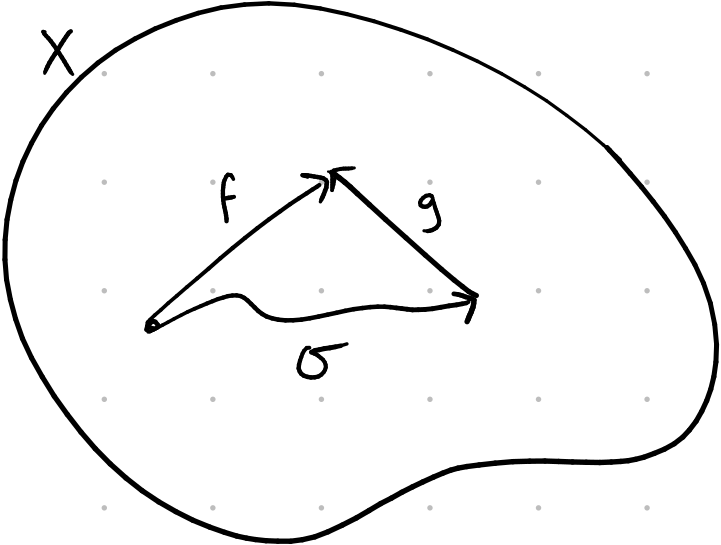
\includegraphics[width=0.25\textwidth]{18_905-200923-1.png}
  \caption{a \(1\)-simplex in \(X\)}%
  \label{fig:locality-1}
\end{figure}
For intuition, if we have some \(\sigma \colon \Delta^1 \to X\),
we can consider two other simplices \(f, g\) such that \(f - g - \sigma = 0\)
in \(H_1(X)\), as shown in \cref{fig:locality-1}.
If we let the endpoints of \(f\) and \(g\) be the midpoint of \(\sigma\),
then we will have \(\sigma = f - g\), modulo \(\partial\).
If we repeat this process, we will eventually have simplices that are
\(\mathcal A\)-small.

To make this precise, we will construct a natural transformation
\[
  \$ \colon S_n \to S_n.
\]
In other words, for any \(X \in \cAb\), we will construct a map
\(\$ \colon S_n(X) \to S_n(X)\). To do so, we need to say what it does
to a generator \(\sigma \colon \Delta^n \to X\).

Consider the naturality square
\[
  \begin{tikzcd}
    S_n(\Delta^n) \arrow[r, "\$"] \arrow[d, "S_n(\sigma)"'] &
      S_n(\Delta^n) \arrow[d, "S_n(\sigma)"] \\
    S_n(X) \arrow[r, "\$"'] &
      S_n(X)
  \end{tikzcd}
\]
which commutes if \(\$\) is natural. There is a special \(n\)-simplex
\[
  1_{\Delta^n} \colon \Delta^n \to \Delta^n.
\]
\(1_{\Delta^n} \in S_n(\Delta^n)\) is one of the generators of the
free abelian group.
Note that \(S_n(\sigma)(1_{\Delta^n}) = \sigma \in S_n(X)\).
Naturality says
\[
  \$(\sigma) = S_n(\sigma)(\$(1_{\Delta^n})).
\]
Therefore, if we specify \(\$(1_{\Delta^n})\), then we specify \(\$\).

\begin{figure}
  \centering
  \begin{subfigure}[b]{0.4\textwidth}
    \centering
    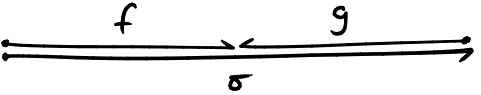
\includegraphics[width=0.7\textwidth]{18_905-200923-2.png}
    \caption{\(\$(1_{\Delta^1})\)}
  \end{subfigure}
  \begin{subfigure}[b]{0.4\textwidth}
    \centering
    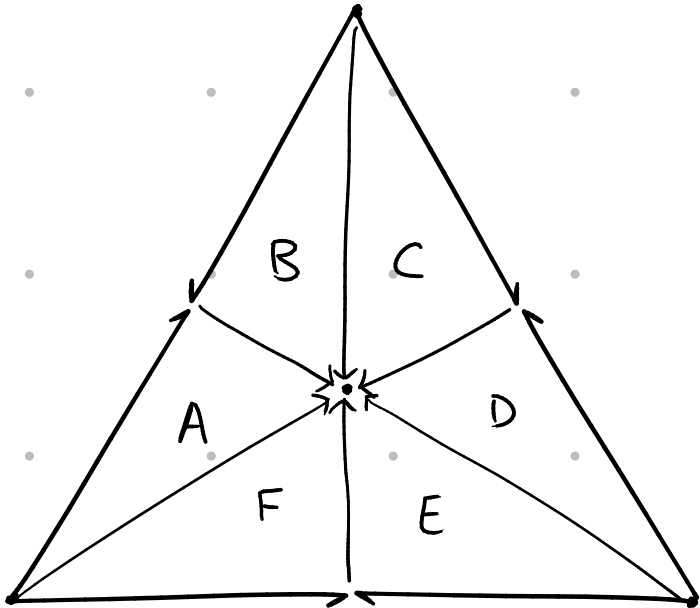
\includegraphics[width=0.7\textwidth]{18_905-200923-3.png}
    \caption{\(\$(1_{\Delta^2})\)}
  \end{subfigure}
  \caption{Diagrams specifying \(\$\)}%
  \label{fig:locality-2}
\end{figure}
\begin{itemize}[nosep]
  \item For \(\Delta^0\), we define \(\$(1_{\Delta^0}) = 1_{\Delta^0}\),
    meaning that if we have \(\Delta^0\), meaning that we do not need to subdivide a point to make it more local.
  \item For \(\Delta^1\), we let \(\$(1_{\Delta^1}) = f - g \in S_1(\Delta^1)\),
    as given by \cref{fig:locality-2}.
  \item For \(\Delta^2\), we let
    \(\$(1_{\Delta^2}) = A-B+C-D+E-F \in S_1(\Delta^2)\),
    also as given by \cref{fig:locality-2}.
\end{itemize}
If we calculate the boundary of these expressions, we get the same thing as
what we would have if we took the boundary of \(\Delta^1\) or \(\Delta^2\).
We think of these expressions as equivalent under homology, but more local.

More generally, to define \(\$(1_{\Delta^n})\), we let \(b\) denote the
center of mass of \(\Delta^n\). We subdivide the boundary of \(\Delta^n\)
according to \(\$\) in one lower dimension, and then connect everything
to \(b\). In particular,
\[
  \$ 1_{\Delta^n} = b \ast \$(\partial 1_{\Delta^n}),
\]
where \(b \ast {-} \colon S_{n-1}(\Delta^n) \to S_n(\Delta^n)\) is the cone
construction for star shaped regions defined for star-shaped regions.

\begin{theorem}
  For any topological space \(X\),
  \[
    \$ \colon S_*(X) \to S_*(X)
  \]
  is a chain map. Furthermore, it is chain homotopic to the identity.
\end{theorem}

\begin{proof}
  Note that we have \(\partial \$ 1_{\Delta^n} = \$ \partial 1_{\Delta^n}\)
  from the definition of the construction of \(\$\).
  It follows by naturailty of \(\$\) that if \(\sigma \colon \Delta^n \to X\)
  is any \(n\)-simplex,
  \[
    \partial \$ \sigma = \partial \$(S_n(\sigma)(1_{\Delta^n}))
      = S_n(\sigma)(\partial \$ 1_{\Delta^n})
      = S_n(\sigma)(\$\partial 1_{\Delta^n})
      = \$ \partial \sigma.
  \]
  Therefore, \(\$\) is a chain map.

  To show that \(\$\) is homotopic to the
  identity, we must define a chain homotopy
  \[
    T \colon S_n(X) \to S_{n+1}(X)
  \]
  from \(\$\) to \(1_{S_*(X)}\). Again by naturality, it suffices to define
  \(T_{1_{\Delta^n}}\). In particular, we define \(T(1_{\Delta^0}) = 0\)
  and for \(n > 0\) define
  \[
    T(1_{\Delta^n}) = b * (
      \$ 1_{\Delta^n}
      - 1_{\Delta^n}
      - T \partial 1_{\Delta^n}
    ) \in S_{n+1}(\Delta^n). \pog
  \]
\end{proof}
 
\begin{example*}
  To give some intuition, \(T(1_{\Delta^1}) \in S_2(\Delta^1)\) is
  the squashed \(\Delta^2\) we drew in \cref{fig:locality-2}.
  In particular, \(T\) specifies how some simplex is related to
  its subdivision.
\end{example*}

Suppose that \(\mathcal A\) is a cover of \(X\). We want to show that
\(S_*^{\mathcal A}(X) \subseteq S_*(X)\) is a homology isomorphism by
repeatedly applying \(\$\).

\begin{lemma}
  Let \(\mathcal A\) be a cover of \(\Delta^n\). Then for any
  \(\sigma \in S_n(\Delta^n)\), there exists \(k \in \NN\) such that
  \(\$^k \sigma = \underbracket{\$\$ \dots \$}_{\text{\(k\) times}} \sigma\)
  is \(\mathcal A\)-small.
\end{lemma}

This is a consequence of the following lemma:
\begin{lemma}[Lebesgue covering]
  Let \(M\) be a compact metric space,
  and let \(\mathcal U\) be an open cover of \(M\).
  Then there is some \(\eps > 0\) such that for all \(x \in M\),
  \(B_\eps(x) \subseteq U\) for some \(U \in \mathcal U\).
\end{lemma}
In particular, we apply this with \(M = \Delta^n\) and
\(\mathcal U = \set{\Int A \mid A \in \mathcal A}\).
More specifically, \(\Delta^n\) has a specific diameter,
and as we subdivide it, the diameter gets smaller until
it is less than \(\eps\).

Here is a more general lemma:
\begin{lemma}
  Let \(\mathcal A\) be a cover of \(X\) and \(\sigma \in S_n(X)\).
  There exists \(k \in \NN\) such that \(\$^k \sigma\) is \(\mathcal A\)-small.
\end{lemma}
The reason why we're able to do this with general spaces that aren't
necessarily compact is because we are only working with
compact subsets of \(X\) at one instance.
\begin{proof}
  Assume without loss of generality that \(\sigma \colon \Delta^n \to X\).
  We can consider \(\sigma\inv (\Int A)\) for \(A \in \mathcal A\),
  which together form an open cover of \(\Delta^n\).
  Then we can apply the previous lemma.
\end{proof}









\end{document}

\documentclass{standalone}
\usepackage{chez}

\begin{document}
\chapter{September 25, 2020}

Let's give some more intuition about the dimension-lowering connecting map
in the long exact sequence.

Let \(A \subseteq X\) be a pair of spaces such that
\[
  H_m(A, X) \iso H_m(X/A, *) \iso H_m(X/A)
\]
for \(m > 0\). We have the long exact sequence
\[
  \begin{tikzcd}
    \cdots \ar[r] &
    H_m(A) \ar[r] &
    H_m(X) \ar[r] &
    H_m(X, A) \iso H_m(X/A) \ar[r, "\partial"] &
    H_{m-1}(A) \ar[r] &
    H_{m-1}(X) \ar[r] &
    \cdots
  \end{tikzcd}
\]
\begin{question}
  What is the geometric intuition of \(\partial\)?
\end{question}
Consider some class \(c \in S_m(X)\) not in \(Z_m(X)\),
i.e.\ \(\partial c \neq 0\).
Suppose that the image of \(c\) under the quotient map
\(S_m(X) \to S_m(X/A)\) is a cycle. Then \(\partial c \in S_{m-1}(X)\)
is actually in the image of \(S_{m-1}(A) \hookrightarrow S_{m-1}(X)\),
and \(\partial c \in Z_{m-1}(A)\).
Therefore, \(\partial c\) represents and element of \(H_{m-1}(A)\).

\begin{example}
  Suppose \(X = [0, 1]\) and \(A = \set{0, 1}\). Then \(X/A \iso S^1\).
  Consider \(\sigma \colon \Delta^1 \to X \in S_1(X)\) where
  \(\sigma \colon e_0 \mapsto 0, e_1 \mapsto 1\).

  In \(S_*(X)\), \(\partial \sigma = \set{1} - \set{0} \neq 0 \in S_0(X)\).
  However, under the quotient \(X \to X/A\), \(\sigma\) is sent to an element
  in \(Z_1(X/A)\). Therefore, \(\sigma\) represents a class in
  \(H_1(X, A) \iso H_1(S^1)\), but its boundary
  \(\partial \sigma = \set{1} - \set{0}\) is a class in \(H_0(A)\).
  Symbolically,
  \begin{align*}
    \cdots \to H_1(S^1) &\to H_0(\set{0, 1}) \to \cdots \\[-1ex]
    \ZZ &\to \ZZ \oplus \ZZ \\[-1ex]
    \sigma &\to (-1, 1).
  \end{align*}
\end{example}

\section{Excision}
Recall that there is a chain homotopy \(T\) from \(\$\) to \(1_{S_*(X)}\).
\begin{corollary}
  There is a natural chain homotopy \(T_k\) from \(\$^k\) to \(1_{S_*(X)}\).
\end{corollary}
\begin{corollary}
  If \(\sigma \in Z_n(X)\), then \(\$^k \sigma\) is equivalent to \(\sigma\)
  modulo boundaries.
\end{corollary}

We will now prove the locality principle.
\begin{theorem*}[\hyperref[thm:locality]{Locality principle}]
  Let \(\mathcal A\) be a cover of \(X\).
  Then \(S_*^{\mathcal A}(X) \subseteq S_*(X)\)
  induces an isomorphism \(H_n^{\mathcal A}(X) \leftrightarrow H_n(X)\).
\end{theorem*}
\begin{proof}
  First we will show surjectivity. Suppose we have some \(c \in Z_n(X)\).
  We want to find an \(\mathcal A\)-small element of \(Z_n(X)\) equivalent
  to \(c\) modulo boundaries. We just use \(\$^k c\) for a sufficiently large
  \(k\), and the Lebesgue covering lemma tells us this works.

  To show injectivity, we can show that the kernel is \(0\).
  In particular, suppose \(c \in Z_n^{\mathcal A}(X)\) is
  an \(\mathcal A\)-small cycle, and \(c = \partial b\) for some
  \(b \in S_{n+1}(X)\). We wish to find some \(b' \in S_{n+1}^{\mathcal A}(X)\)
  such that \(\partial b' = c\). We can select \(k\) such that \(\$^k b\) is
  \(\mathcal A\)-small. Note that
  \begin{align*}
    \partial(\$^k b) - c &= \partial ((\$^k - 1_{S_{n+1}(X)})(b)) \\
      &= \partial((\partial T_k + T_k \partial) b) \\
      &= \partial \partial T_k b + \partial (T_k \partial b) \\
      &= 0 + \partial (T_k c).
  \end{align*}
  Rearranging,
  \[
    c = \partial(\$^k b - T_k c).
  \]
  We finish by the following:
  \begin{lemma*}
    If \(c \in S_n(X)\) is \(\mathcal A\)-small, then
    \(T_k c \in S_{n+1}(X)\) is also \(\mathcal A\)-small.
  \end{lemma*}
  \begin{proof*}{Lemma proof}
    Without loss of generality assume that
    \(c = \sigma\) is an \(\mathcal A\)-small \(n\)-simplex.
    We can represent it as a composite
    \(\Delta^n \overset{\sigma'}\to A \overset{i}\to X\)
    where \(A \in \mathcal A\), where
      \(\sigma'\) denotes the map \(\Delta^n \to A\) and
      \(i\) is the inclusion of \(A\) into \(X\).
    Note that \(\sigma = S_n(i)(\sigma')\), so
    \(T_k \sigma = (S_{n+1}(i))(T_k \sigma')\)
    by the naturailty of \(T_k\).
    We know that \(T_k \sigma\) is the image of
    some \(T_k \sigma' \in S_{n+1}(A)\), so
    \(T_k \sigma\) is \(\mathcal A\)-small.
  \end{proof*}
  This concludes the proof of the locality principle.
\end{proof}

Now we can prove excision.
\begin{theorem*}[Excision]
  Suppose \(U \subseteq A \subseteq X\) is excisive, i.e.\
  \(\ol U \subseteq \Int A\). Then the map \((X - U, A - U) \to (X, A)\)
  induces homology isomorphisms.
\end{theorem*}
\begin{proof}
  Note that the condition \(\ol U \subseteq \Int A\) is equivalent to
  \[
    \Int A \union \Int (X - U) = X.
  \]
  Let \(B \coloneqq X - U\). Then \(\set{A, B}\) is a cover of \(X\).
  We can rewrite \((X - U, A - U) = (B, A \intersect B)\), so we want to show
  that the inclusion
  \[
    S_*(B, A \intersect B) \hookrightarrow S_*(X, A)
  \]
  induces homology isomorphisms.
  Note the diagram of a map of short exact sequences of chain complexes
  \[
    \begin{tikzcd}
      0 \ar[r]                                                      &
        S_*(A) \ar[r] \ar[d, equal]                                 &
        S_*^{\mathcal A}(X) \ar[r], \ar[d, hook]                    &
        S_*^{\mathcal A}(X)/S_*^{\mathcal A}(A) \ar[r] \ar[d, hook] &
        0                                                           \\
      0 \ar[r]                                                      &
        S_*(A) \ar[r]                                               &
        S_*(X) \ar[r]                                               &
        \underset{\mathclap{= S_*(X)/S_*(A)}}{S_*(X, A)} \ar[r]     &
        0
    \end{tikzcd}
  \]
  We can obtain a map of long exact sequences of homology groups
  \[
    \begin{tikzcd}
      \cdots \ar[r]                                               &
      H_m(A) \ar[r] \ar[d]                                        &
      H_m^{\mathcal A}(X) \ar[r] \ar[d]                           &
      H_m(S_*^{\mathcal A}(X) / S_*(X)) \ar[r, "\partial"] \ar[d] &
      H_{m-1}(A) \ar[r] \ar[d]                                    &
      H_{m-1}^{\mathcal A}(X) \ar[r] \ar[d]                       &
      \cdots                                                      \\
      \cdots \ar[r]                                               &
      H_m(A) \ar[r]                                               &
      H_m(X) \ar[r]                                               &
      H_m(S_*(X) / S_*(X)) \ar[r, "\partial"]                     &
      H_{m-1}(A) \ar[r]                                           &
      H_{m-1}^{\mathcal A}(X) \ar[r]                              &
      \cdots
    \end{tikzcd}
  \]
  By locality, the \(H_m^{\mathcal A}(X) \to H_m(X)\) and
  \(H_{m-1}^{\mathcal A}(X) \to H_{m-1}(X)\) maps are isomorphisms.
  By the five-lemma,
  \[
    H_m(S_*^{\mathcal A}(X) / S_*(X)) \to H_m(X, A)
  \]
  is also an isomorphism. Therefore,
  \(S_*^{\mathcal A}(X) / S_*(A) \to S_*(X) / S_*(A)\)
  induces homology isomorphisms \(H_m(S_*(X)/S_*(A)) \iso H_m(X, A)\).
  Then observe
  \begin{align*}
    S_n^{\mathcal A}(X) / S_n(A) &= \frac{S_n(A) + S_n(B)}{S_n(A)} \\
      &= \frac{S_n(B)}{S_n(A) \intersect S_n(B)} \\
      &= \frac{S_n(B)}{S_n(A \intersect B)} \\
      &= \frac{S_n(X - U)}{S_n(A - U)}. \pog
  \end{align*}
\end{proof}

\begin{corollary}
  Let \((X, A)\) be a pair of spaces and let \(B \subseteq X\) be a subspace
  such that
  \begin{enumerate}[nosep]
    \item \(\overline A \subseteq \Int B\) and
    \item \(A \to B\) is a deformation retract.\label{item-def-retract}
  \end{enumerate}
  Then for all \(m\), \(H_m(X, A) \to H_m(X/A, *)\) is an isomorphism.
\end{corollary}
\begin{proof}
  Consider the commutative diagram in \(\cTop_2\)
  \[
    \begin{tikzcd}
      (X, A) \arrow[r, "i"] \arrow[d] &
        (X, B) \arrow[r, leftarrow, "j"] \arrow[d] &
        (X - A, B - A) \arrow[d, "k"] \\
      (X/A, *) \arrow[r, "\ol i"] &
        (X/A, B/A) \arrow[r, leftarrow, "\ol j"] &
        (X/A - *, B/A - *)
    \end{tikzcd}
  \]
  We can check that each labeled arrow induces a homology isomorphism:
  \begin{itemize}
    \item \(k\) is a homeomorphism in \(\cTop_2\).
    \item \(j\) is an excision
    \item \(i\) is a homology isomorphism by \cref{item-def-retract} and
      the homotopy invariance of homology.
    \item \(\ol j\) is an excision.
    \item \(\ol i\) is also a deformation detract, obtained from
    the given retract \(B \times I \to B\) by quotienting out by \(A\).
  \end{itemize}
  Since all of the maps along the edge induce an homology isomorphism,
  the map on the left also induces a homology isomorphism.
\end{proof}

This concludes the proof of all of the Eilenberg-Steenrod axioms.





\end{document}

\documentclass{standalone}
\usepackage{chez}

\begin{document}
\chapter{September 28, 2020}

Here is a summary of what we have:
\begin{theorem}[Eilenberg-Steenrod axioms]
  There are functors \(H_n \colon \cTop_2 \to \cAb\). If \(X\) is
  a topological space, we write \(H_n(X) \coloneqq H_n(X, \nullset)\).

  There are natural transformations
  \(\partial \colon H_n(X, A) \to H_{n-1}(A)\) where:
  \begin{itemize}
    \item If \(f_0, f_1 \colon (X, A) \to (Y, B)\) are homotopic, then
      \(H_n(f_0) H_n(f_1)\).
    \item Excisions in \(\cTop_2\) induce isomorphisms on \(H_n\).
    \item For any pair \((X, A)\), the sequence
      \[
        \begin{tikzcd}
          \cdots \ar[r] &
          H_{n+1}(X, A) \ar[r, "\partial"] &
          H_n(A) \ar[r] &
          H_n(X) \ar[r] &
          H_n(X, A) \ar[r, "\partial"] &
          \cdots
        \end{tikzcd}
      \]
      is exact.
    \item \(\displaystyle H_n\parens[\Big]{\smash{\coprod_{i \in I}} X_i}
      = \bigoplus_{i \in I} H_n(X_i)\).
    \item (Dimension axiom) \(H_n(*) = \begin{cases*}
        \ZZ & if \(n = 0\) \\[-1ex] 0 & otherwise.
      \end{cases*}\)
  \end{itemize}
\end{theorem}

An application of excision is that, in favorable conditions,
\(H_n(X, A) \iso H_n(X/A, *) \iso H_n(X, A)\) if \(n > 0\).

\section{Mayer-Vietoris sequence}
One more practical tool for computing the homology of topological spaces is
the \vocab{Mayer-Vietoris sequence}.

Suppose \(X\) is a space and \(\mathcal A = \set{A, B}\) is a cover of \(X\).
Let us label the inclusions
\begin{align*}
  i &\colon A \intersect B \hookrightarrow A \\
  j &\colon A \intersect B \hookrightarrow B \\
  k &\colon A \hookrightarrow X \\
  l &\colon B \hookrightarrow X.
\end{align*}
\begin{theorem}[Mayer-Vietoris]
  There is a long exact sequence
  \[
    \begin{tikzcd}
    	\cdots \ar[r] &
    	H_{n+1}(X) \ar[r, "\partial"] &
    	H_n(A \intersect B) \ar[rr, "H_n(i) \oplus H_n(j)"] &&
    	H_n(A) \oplus H_n(B) \ar[rr, "H_n(k) - H_k(l)"] &&
    	H_n(X) \ar[r, "\partial"] &
    	H_{n-1}(A \intersect B) \ar[r] &
    	\cdots
    \end{tikzcd}
  \]
\end{theorem}
\begin{proof}
  Consider the short exact sequence of chain complexes
  \[
    \begin{tikzcd}
    	0 \ar[r] &
    	S_*(A \intersect B) \ar[rr, "{S_*(i, j)}"] &&
    	S_*(A) \oplus S_*(B) \ar[rr, "S_*(k) - S_*(l)"] &&
    	S_*^{\mathcal A}(X) \ar[r] &
    	0
    \end{tikzcd}
  \]
  By the locality principle, \(H_n(S_*^{\mathcal A}(X)) \iso H_n(X)\),
  so we obtain the Mayer-Vietoris sequence from the long exact sequence
  associated to a short exact sequence of chain complexes.
\end{proof}

\begin{example}
  \begin{minipage}{0.68\textwidth}
    Consider the sphere \(S^2\), with the cover \(\mathcal A = \set{A, B}\),
    where
    \begin{align*}
      A &= \set{(x, y, z) \in \RR^3 \mid z > -1/2}, \\
      B &= \set{(x, y, z) \in \RR^3 \mid z < 1/2},
    \end{align*}
    as in the diagram to the right.
  \end{minipage}
  \begin{minipage}{0.28\textwidth}
    \centering
    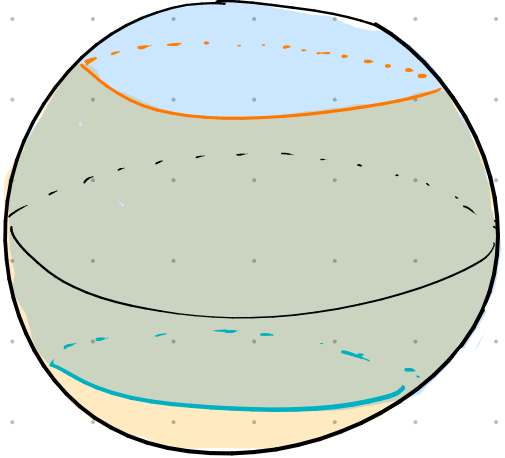
\includegraphics[width=0.55\textwidth]{18_905-200928-1.png}
  \end{minipage}
  \smallskip

  We have the Mayor-Vietoris sequence
  \[
    \begin{tikzcd}
    	H_2(A) \oplus H_2(B) \ar[r] &
    	H_2(S^2) \ar[r, "\partial"] &
    	H_1(A \intersect B) \ar[r] &
    	H_1(A) \oplus H_1(B)
    \end{tikzcd}
  \]
  We know that \(A\) and \(B\) are homotopy equivalent to a point, so
  \(H_2(A) \oplus H_2(B) \iso 0 \oplus 0 \iso 0\).
  Similarly, we know that \(H_1(A) \oplus H_1(B) \iso 0\).
  We also know that
  \(A \intersect B\) is homotopy equivalent to \(S^1\), so
  \(H_1(A \intersect B) = \ZZ\).
  Therefore, the exact sequence is
  \[
    \begin{tikzcd}
    	0 \ar[r] &
    	H_2(S_2) \ar[r, "\partial"] &
    	\ZZ \ar[r] &
    	0
    \end{tikzcd}
  \]
  Exactness says that \(\partial\) is both injective and surjective,
  so \(H_2(S^2) \iso \ZZ\).
\end{example}

\begin{example}
  Let \(T^2 \iso S^1 \times S^1\) be the torus,
  and let \(\mathcal A = \set{A, B}\) be
  the cover as defined by the image:
  \begin{center}
    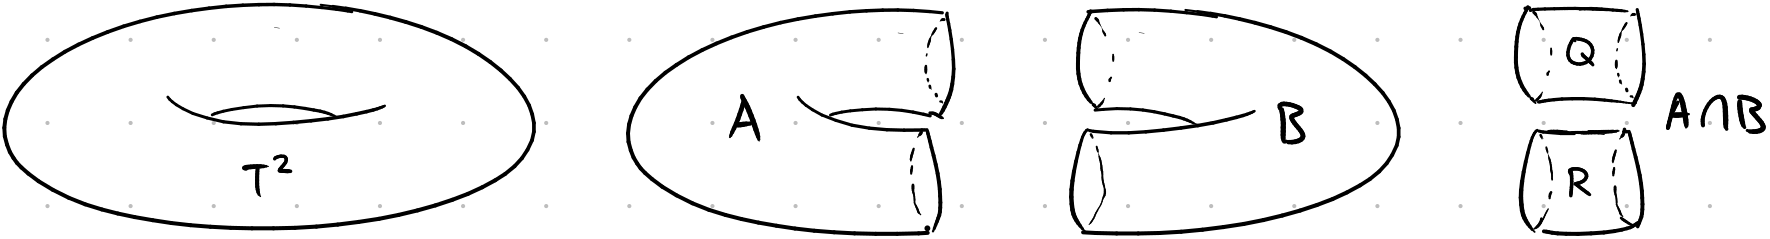
\includegraphics[width=0.8\textwidth]{18_905-200928-2.png}
  \end{center}

  We have the long exact sequence
  \[
    \begin{tikzcd}[column sep=small]
    	H_2(A) \oplus H_2(B) \ar[r] &
    	H_2(T^2) \ar[r, "\partial"] &
    	H_1(A \intersect B) \ar[r] &
    	H_1(A) \oplus H_1(B) \ar[r] &
    	H_1(T^2) \ar[r, "\partial"] &
    	H_0(A \intersect B) \ar[r] &
    	H_0(A) \oplus H_0(B)
    \end{tikzcd}
  \]
  Note that \(A\) and \(B\) are homeomorphic to an annulus,
  and therefore they are homotopy equivalent to \(S^1\).
  This simplifies our sequence to
  \[
    \begin{tikzcd}[column sep=small]
    	0 \ar[r] &
    	H_2(T^2) \ar[r, "\partial"] &
    	H_1(A \intersect B) \ar[r] &
    	\ZZ \oplus \ZZ \ar[r] &
    	H_1(T^2) \ar[r, "\partial"] &
    	H_0(A \intersect B) \ar[r] &
    	\ZZ \oplus \ZZ
    \end{tikzcd}
  \]
  Since \(A \intersect B\) has two path components,
  \(H_0(A \intersect B) = \ZZ \oplus \ZZ\).
  Also, since \(A \intersect B \simeq S^1 \sqcup S^1\),
  we know \(H_1(A) \oplus H_1(B) \iso \ZZ \oplus \ZZ\).
  \[
    \begin{tikzcd}[column sep=small]
    	0 \ar[r] &
    	H_2(T^2) \ar[r, "\partial"] &
    	\ZZ \oplus \ZZ \ar[r] &
    	\ZZ \oplus \ZZ \ar[r] &
    	H_1(T^2) \ar[r, "\partial"] &
    	\ZZ \oplus \ZZ \ar[r] &
    	\ZZ \oplus \ZZ
    \end{tikzcd}
  \]
  This is not enough to understand the homology groups of the torus,
  so we will need to look at some of the maps.
  Consider the map \(g \colon H_0(A \intersect B) \to H_0(A) \oplus H_0(B)\).
  This maps the path component \(Q\), represented by
  \((1, 0) \in \ZZ \oplus \ZZ \iso H_0(A \intersect B)\),
  to \((1, 1)\) because \(Q \subseteq A, B\).
  Similarly \(R \mapsto (1, 1)\).
  Therefore, \(g \colon (x, y) \mapsto (x+y, x+y)\).

  Now consider \(f \colon H_1(A \intersect B) \to H_1(A) \oplus H_1(B)\).
  To think about this, we can consider the natural chain
  \[
    Q \to A \intersect B \to A \sqcup B \to A,
  \]
  and applying \(H_1\) gives
  \[
    \ZZ \to \ZZ \oplus \ZZ \to \ZZ \oplus \ZZ \to \ZZ.
  \]
  This maps \(1 \mapsto (1, 0) \mapsto f(1, 0) \mapsto 1\),
  because \(Q \to A\) is a deformation retract.
  Similarly, \(Q \to B\) is a deformation retract, so \(f(1, 0) = (1, 1)\).
  If we replace \(Q\) with \(R\), we also get \(f(0, 1) = (1, 1)\).
  Therefore, \(f \colon (x, y) \mapsto (x+y, x+y)\).

  This gives the following long exact sequence
  \[
    \begin{tikzcd}[column sep=small, row sep=0.1em]
    	H_2(A) \oplus H_2(B) \ar[r] &
        H_2(T^2) \ar[r] &
        H_1(A \intersect B) \ar[r, "f"] &
        H_1(A) \oplus H_1(B) \ar[r, "r"] &
        H_1(T^2) \ar[r, "s"] &
        H_0(A \intersect B) \ar[r, "g"] &
        H_0(A) \oplus H_0(B) \\
    	0 \oplus H_2(B) \ar[r] &
        H_2(T^2) \ar[r] &
        \ZZ \oplus \ZZ \ar[r] &
        \ZZ \oplus \ZZ \ar[r] &
        H_1(T^2) \ar[r] &
        \ZZ \oplus \ZZ \ar[r] &
        \ZZ \oplus \ZZ \\
    	&
        &
        (x, y) \ar[r, mapsto] &
        (x+y, x+y) &
        &
        (x, y) \ar[r, mapsto] &
        (x+y, x+y)
    \end{tikzcd}
  \]

  Exactness at \(H_2(T^2)\) tells us that
  \(H_2(T^2) \hookrightarrow \ZZ \oplus \ZZ\) is an injection.
  Exactness at \(H_1(A \intersect B) \iso \ZZ \oplus \ZZ\) tells us that
  \(H_2(T) \iso \ker f \iso \ZZ{(1, -1)} \iso \ZZ\).
  Therefore, we have computed \(H_2(T^2) \iso \ZZ\).

  To compute \(H_1(T^2)\),
  note that exactness at \(H_1(A) \oplus H_1(B)\)
  tells us that \(\ker r = \img f \iso \ZZ\),
  and exactness at \(H_0(A \intersect B)\) tells us that
  \(\ker g = \img s \iso \ZZ\).
  Therefore, \(H_1(T^2)/\ZZ \iso \ZZ \implies H_1(T^2) \iso \ZZ \oplus \ZZ\).
\end{example}

\begin{figure}
  \centering
  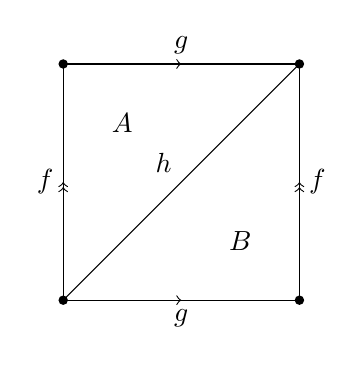
\begin{tikzpicture}[scale=3]
    \begin{scope}[decoration={markings, mark=at position 0.5 with {\arrow{>}}}]
      \draw[postaction={decorate}] (0, 0) -- (1, 0) node[midway, below]{\(g\)};
      \draw[postaction={decorate}] (0, 1) -- (1, 1) node[midway, above]{\(g\)};
    \end{scope}
    \begin{scope}[decoration={markings, mark=at position 0.5 with {\arrow{>>}}}]
      \draw[postaction={decorate}] (1, 0) -- (1, 1) node[midway, right]{\(f\)};
      \draw[postaction={decorate}] (0, 0) -- (0, 1) node[midway, left ]{\(f\)};
    \end{scope}
    \draw (0, 0) -- (1, 1) node[midway, above left]{\(h\)};

    \node () at (1/4, 3/4) {\(A\)};
    \node () at (3/4, 1/4) {\(B\)};

    \fill (0, 0) circle[radius=0.02];
    \fill (0, 1) circle[radius=0.02];
    \fill (1, 0) circle[radius=0.02];
    \fill (1, 1) circle[radius=0.02];
  \end{tikzpicture}
  \caption{Fundamental polygon of torus}\label{fig:torus-fundamental-polygon}
\end{figure}
A more combinatorial way to think about the torus as a square
with the edges identified like in \cref{fig:torus-fundamental-polygon}.
This represents a semisimplicial set
\[
  \begin{tikzcd}
  	\ZZ\{A, B\} \ar[r] &
  	\ZZ\{f, g, h\} \ar[r] &
  	\ZZ\{x\}
  \end{tikzcd}
\]
which lets us find the homology more combinatorially.
The first map maps \(A \mapsto f + g - h\) and \(B \mapsto g + f - h\).
The second map maps \(f, g, h \mapsto 0\), since all four of the points
are the same.

Our goal in the next few classes is to show that no matter how we cut up
the space.



\end{document}

\documentclass{standalone}
\usepackage{chez}

\begin{document}
\chapter{September 30, 2020}

\begin{definition}
  Let \(\mathcal C\) be a category and let
  \[
    \begin{tikzcd}
      A \arrow[r, "f"] \arrow[d, "g"'] &
        B \\
      C
    \end{tikzcd}
  \]
  be a diagram in \(\mathcal C\).
  A \vocab{pushout} of this diagram is a commuting square
  \[
    \begin{tikzcd}
      A \arrow[r, "f"] \arrow[d, "g"'] &
        B \arrow[d, "p_B"] \\
      C \arrow[r, "p_C"'] & P
    \end{tikzcd}
  \]
  such that for any other commuting square
  \[
    \begin{tikzcd}
      A \arrow[r, "f"] \arrow[d, "g"'] &
        B \arrow[d, "p_B'"] \\
      C \arrow[r, "p_C'"'] & P'
    \end{tikzcd}
  \]
  there is a unique map \(p \colon P \to P'\) with \(p \circ p_C = p_C'\)
  and \(p \circ p_B = p_B'\).
\end{definition}

\subsection{Pushouts in \texorpdfstring{\(\cTop\)}{Top}}
Suppose
\(
  \begin{tikzcd}[cramped, column sep=small, row sep=scriptsize]
    A \arrow[r, "f"] \arrow[d, "g"'] &
      B \\
    C
  \end{tikzcd}
\)
is a diagram in \(\cTop\).
Then the pushout
\[
  \begin{tikzcd}
    A \arrow[r, "f"] \arrow[d, "g"'] &
      B \arrow[d, "p_B"] \\
    C \arrow[r, "p_C"'] & P
  \end{tikzcd}
\]
has \(P = (B \sqcup C) / (\text{\(f(a) = g(a)\) for all \(a \in A\)})\),
where \(p_B \colon B \to P\) is the composite of the natural inclusion
and the quotient map \(B \to B \sqcup C \to P\).

\begin{example}
  The pushout of
  \(
    \begin{tikzcd}[column sep=scriptsize]
      C & \nullset \ar[l] \ar[r] & B
    \end{tikzcd}
  \)
  is just the disjoint union \(B \sqcup C\).
\end{example}

\begin{example}
  The pushout of
  \(
    \begin{tikzcd}[column sep=scriptsize]
      * & A \ar[l] \ar[r, "f"] & B
    \end{tikzcd}
  \)
  is the quotient \(P = B / \img f\).
\end{example}


\begin{definition}
  If there is a pushout square
  \[
    \begin{tikzcd}
      \coprod_{i \in I} S^{n-1} \arrow[r] \arrow[d, hook] &
        B \arrow[d] \\
      \coprod_{i \in I} D^n \arrow[r] &
        P
    \end{tikzcd}
  \]
  then we say that \(P\) is obtained from \(B\) by attaching \(n\)-cells.
\end{definition}
The idea is that we take \(B\), and find copies of \(S^{n-1}\) inside \(B\).
At those points, we glue copies of \(D^n\) such that the boundary of
the disks are the copies of \(S^{n-1}\) we selected.

\begin{example}
  The following pushout
  \[
    \begin{tikzcd}
      S^1 \sqcup S^1 \arrow[r] \arrow[d] &
        * \arrow[d] \\
      D^2 \sqcup D^2 \arrow[r] &
        P
    \end{tikzcd}
  \]
  is obtained from the point by attaching two \(2\)-cells.
  Geometrically, P looks like this:
  \begin{center}
    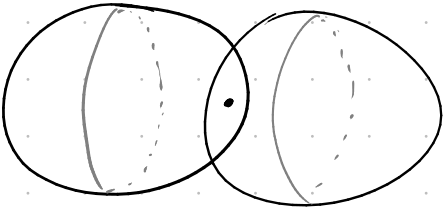
\includegraphics[width=0.25\textwidth]{18_905-200930-1.png}
  \end{center}
\end{example}
\begin{example}
  \begin{center}
    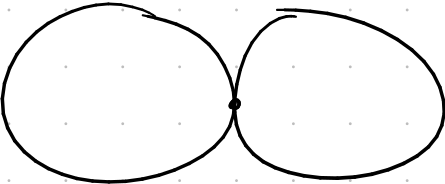
\includegraphics[width=0.2\textwidth]{18_905-200930-2.png}
  \end{center}
  The example one dimension lower is the figure-8 space,
  which is obtained from attaching two \(1\)-cells to a point, i.e.
  \[
    \begin{tikzcd}
      S^0 \sqcup S^0 \arrow[r] \arrow[d] &
        * \arrow[d] \\
      D^1 \sqcup D^1 \arrow[r] &
        P_8
    \end{tikzcd}
  \]
\end{example}

Another way to describe the figure-8 space \(P_8\)
is to say that it is homeomorphic to
\begin{center}
  \begin{tikzpicture}[scale=2]
    \begin{scope}[decoration={markings, mark=at position 0.5 with {\arrow{>}}}]
      \draw[postaction={decorate}] (1, 0) -- (1, 1) node[midway, right]{\(a\)};
      \draw[postaction={decorate}] (0, 0) -- (0, 1) node[midway, left ]{\(a\)};
    \end{scope}
    \begin{scope}[decoration={markings, mark=at position 0.5 with {\arrow{>>}}}]
      \draw[postaction={decorate}] (0, 0) -- (1, 0) node[midway, below]{\(b\)};
      \draw[postaction={decorate}] (0, 1) -- (1, 1) node[midway, above]{\(b\)};
    \end{scope}

    \fill (0, 0) circle[radius=0.02];
    \fill (0, 1) circle[radius=0.02];
    \fill (1, 0) circle[radius=0.02];
    \fill (1, 1) circle[radius=0.02];
  \end{tikzpicture}
\end{center}
where the square is not filled in.
Then, we see that there is a continuous map \(r \colon S^1 \to P_8\)
called \(a b a\inv b\inv\).
We can glue a \(2\)-cell to \(P_8\) by using \(r\) as the boundary.
\[
  \begin{tikzcd}
    S^1 \arrow[r, "r"] \arrow[d, hook] &
      P_8 \arrow[d] \\
    D^2 \arrow[r] & P
  \end{tikzcd}
\]
However, this just fills in the square,
so what we get is the torus \(P = T^2\).

\begin{definition}
  A \vocab{CW complex} \(X\) is a space with a sequence of subspaces
  \[
    \nullset = \Sk_{-1} X
      \subseteq \Sk_0 X
      \subseteq \Sk_1 X
      \subseteq \Sk_2 X
      \subseteq \dots \subseteq X
  \]
  such that
  \begin{itemize}
    \item \(X\) is the union of its \vocab{skeleta} \(\Sk_n X\)
    \item there exist pushout diagrams
    \[
    \begin{tikzcd}
      \coprod_{i \in I_n} S^{n-1} \arrow[r] \arrow[d, hook] &
        \Sk_{n-1} X \arrow[d] \\
      \coprod_{i \in I_n} D^n \sqcup D^1 \arrow[r] &
        \Sk_n X
    \end{tikzcd}
    \]
    i.e.\ \(\Sk_n X\) is obtained from \(\Sk_{n-1} X\)
    by attaching \(n\)-cells.
  \end{itemize}
\end{definition}

\begin{remark}
  Tomorrow is October so we can start talking about skeletons.
\end{remark}

\begin{example}
  The torus \(T^2\) can be given the structure of a CW complex with
  \begin{align*}
    \Sk_0 T^2 &= * \\
    \Sk_1 T^2 &= P_8 \\
    \Sk_2 T^2 &= T \\
    \Sk_3 T^2 &= T. \\
    \MTFlushSpaceAbove
    &\vdotswithin{=}
  \end{align*}
\end{example}

\begin{definition}
  A CW-complex is \vocab{finite dimensional} if \(\Sk_n X = X\) for some \(n\).
  The \vocab{dimension} of \(X\) is the smallest \(n\) for which this is true.
\end{definition}

This means that \(T^2\) is two dimensional.
However, a generic CW complex may he infinite-dimensional.

\begin{definition}
  A CW complex is of \vocab{finite type} if each \(I_n\) is finite.
\end{definition}

\begin{definition}
  A CW complex is \vocab{finite} if
    it is finite dimensional
    and of finite type.
\end{definition}

Here are some facts from point set topology that
we will not check, but are true.
\begin{lemma}
  \begin{itemize}[nosep]
    \item Any CW complex is Hausdorff.
    \item A CW complex \(X\) is compact if and only if \(X\) is finite.
    \item Any compact smooth manifold can be given some finite
      CW complex structure.
  \end{itemize}
\end{lemma}

Note that we can organize CW complexes into a category \(\cCWcomp\) where
the morphisms are diagrams
\[
  \begin{tikzcd}[row sep=small]
    \vdots & \vdots \\
    \Sk_{n+1} X \ar[r] \ar[u, symbol=\subseteq]
      & \Sk_{n+1} Y \ar[u, symbol=\subseteq] \\
    \Sk_{n} X \ar[r] \ar[u, symbol=\subseteq]
      & \Sk_{n} Y \ar[u, symbol=\subseteq] \\
    \vdots  \ar[u, symbol=\subseteq]
      & \vdots  \ar[u, symbol=\subseteq] \\
    \Sk_{0} X \ar[r] \ar[u, symbol=\subseteq]
      & \Sk_{0} Y \ar[u, symbol=\subseteq]
  \end{tikzcd}
\]

There is a functor
\[
  \mathcal U \colon \cCWcomp \to \cTop
\]
that ignores the skeletal structure and just returns the union of the skeleta.

There is also a functor
\[
  \Fun(\Deltainj^\op, \cSet) \to \cCWcomp
\]
where we consider the simplicial sets geometrically,
i.e.\ if \(X_\bullet\) is a simplicial set,
\(X_n\) is the set of \(n\)-cells in the corresponding CW complex,
and the \(d\) maps give the boundaries of the gluing.

The composite functor
\[
  \Fun(\Deltainj^\op, \cSet) \to \cCWcomp \overset{U}\to \cTop
\]
is called the \vocab{geometric realization}.

The goal is to understand \(H_n\) of a geometric realization.
In particular We want to confirm that the homology of
a semisimplicial set is the same as its geometric realization.

\begin{example}
  \(S^n\) can be given a CW structure with one \(0\)-cell and one \(n\)-cell.
  In particular, there is a pushout diagram
  \[
    \begin{tikzcd}
      S^{n-1} \arrow[r] \arrow[d, hook] &
        * \arrow[d] \\
      D^n \arrow[r] &
        S^n
    \end{tikzcd}
  \]
  However, we can form a different CW structure on \(S^n\):
  \begin{align*}
    \Sk_{-1} S^n &= \nullset \\
    \Sk_0 S_n &= * \sqcup * = S^0 \\
    \Sk_1 S_n &= S^1 \\
    \shortvdotswithin{=}
    \Sk_n S_n &= S^n \\
    \Sk_{n+1} S_n &= S^n \\
    \MTFlushSpaceAbove
    &\vdotswithin{=}
  \end{align*}
  where to get from \(\Sk_{k-1} S^n\) to \(\Sk_n S^n\),
  we glue two \(k\)-cells as ``hemispheres''.
\end{example}

Note that there is a CW complex \(S^\infty\) which has
\(\Sk_n S^\infty = S_n\) for all \(n\).
Note that \(S^\infty\) is of finite type, but is not finite.



\end{document}

\documentclass{standalone}
\usepackage{chez}

\begin{document}
\chapter{October 02, 2020}

Recall that
\[
  H_q(S^n) = \begin{cases*}
    \ZZ & if \(q = 0, n\) \\[-1ex]
    0 & otherwise.
  \end{cases*}
\]
We claim that
\[
  H_q(S^\infty) = \begin{cases*}
    \ZZ & if \(q = 0\) \\[-1ex]
    0 & otherwise.
  \end{cases*}
\]

\begin{proposition}
  \(S^\infty\) is contractible.
\end{proposition}
\begin{proof}
  Since \(S^\infty = \bigunion S^n\),
  a point \(x \in S^\infty\) is a sequence
  \(x = (x_0, x_1, x_2, \dots)\) such that
  \begin{enumerate}[nosep]
    \item \(x_n = 0\) for all sufficiently large \(n\),
    \item \(\sum x_i^2 = 1\).
  \end{enumerate}
  Consider \(* \overset{f}\to S^\infty\)
  that picks out \((1, 0, 0, \dots)\).
  Also consider the map \(S^\infty \overset{g}\to *\)
  that maps every point in \(S^\infty\) to \(*\).

  We will show that \(f \circ g \simeq 1_{S^\infty}\)
  and \(g \circ g \simeq 1_{*}\).
  The second homotopy is easy because there
  is only one point that \(*\) can go to.
  To show the first, note that
  \(f \circ g \colon S^\infty \to S^\infty\)
  sends every point to \((1, 0, 0, \dots)\).

  Consider another map
  \begin{align*}
    T \colon& S^\infty \to S^\infty \\
      & (x_0, x_1, x_2, \dots) \mapsto (0, x_0, x_1, \dots).
  \end{align*}
  We will show that \(f \circ g \simeq T \simeq 1_{S^\infty}\).
  In particular, the homotopy \(T \simeq 1_{S^\infty}\) can be shown by
  \begin{align*}
    h \colon& S^\infty \times [0, 1] \to S^\infty \\
      & (x, t) \mapsto \frac{t x + (1-t) T x}{\norm{t x + (1-t) T x}}.
  \end{align*}
  This is well-defined and continues because \(t x + (1-t) T x\)
  is never the origin, since the first nonzero coordinate in \(T x\)
  occurs after the first nonzero coordinate in \(x\).

  We can show the homotopy \(T \simeq f \circ g\) with the homotopy
  \[
    h(x, t) = \frac{t T x + (1 - t)(1, 0, 0, \dots)}
                   {\norm{t T x + (1 - t)(1, 0, 0, \dots)}}.
  \]
  This is also well-defined because the first coordinate is always positive
  except for \(t = 1\), for which the value is \(T x\).
\end{proof}

This proof technique is called a swindle,
where in infinite dimensions we shift all the coordinates,
which works because there are an infinite number of dimensions.

\section{Real projective space}
For some \(k \in \NN\), \(\RP^k\) is \vocab{real projective \(k\)-space},
defined to be \(\RP^k \coloneq S^k / (x \sim -x)\).

\begin{example}
  \(\RP^0\) is \(S^0 / (x \sim -x)\), which is just \(*\).

  \(\RP^1\) is \(S^1 / (x \sim -x)\), which is another \(S^1\).

  \(\RP^2\) is \(S^2 / (x \sim x)\)
  is the sphere with antipodal points identified,
  but is hard to describe in more familiar terms.
  In fact, this is not embeddable in \(3\)-dimensional space.
\end{example}

Note that the inclusion of the equator \(S^k \to S^{k+1}\)
is compatible with \(x \mapsto -x\).
In particular, there are inclusions
\[
  \nullset \subseteq
  \RP^0 \subseteq
  \RP^1 \subseteq
  \RP^2 \subseteq \cdots
\]
In fact, this is a CW complex:
\[
  \begin{tikzcd}
    S^{k-1} \arrow[r] \arrow[d, hook] &
      \RP^{k-1} \arrow[d] \\
    D^k \arrow[r] &
      \RP^k
  \end{tikzcd}
\]
where \(S^{k-1} \to \RP^{k-1}\) is the quotient map,
\(S^{k-1} \to D^k\) is the boundary of \(D^k\),
where we think of \(D^k\) as the upper hemisphere of \(S^k\).

Then, we can define \(\RP^\infty = \bigunion \RP^n\), which is a finite type,
but not a finite CW complex.
Unlike \(S^\infty\), \(\RP^\infty\) is not contractible.


\section{Homology of CW complexes}
Before we start taking about homologies, let's introduce one more space.
\begin{definition}
  A \vocab{wedge of \(k\)-spheres} is a space, denoted by
  \(\bigvee_{i \in I} S^k\),
  consisting of \(\norm{I}\) different \(k\)-spheres all meeting
  at a single point.
\end{definition}

\begin{example}
  The figure eight is a wedge of two \(1\)-spheres,
  the wedge of three \(1\)-spheres is
  \begin{center}
    
\includegraphics[width=0.15\textwidth]{18_905-201002-1.png}
  \end{center}
  and the wedge of two \(2\)-spheres is
  \begin{center}
    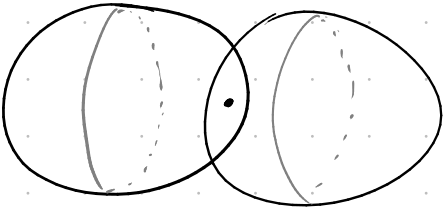
\includegraphics[width=0.25\textwidth]{18_905-200930-1.png}
  \end{center}
\end{example}
More formally, we can say
\(
  \bigvee_{i \in I} S^k =
  \left.\coprod_{i \in I} S^k \middle /
    \coprod_{i \in I} *\right.
\).

We can ask what are the reduced homology groups
\[
  \tilde H_q \parens[\Big]{\bigvee_{i \in I} S^k}
    = H_q \parens[\Big]{\bigvee_{i \in I} S^k, *}
    = H_q \parens[\Big]{\coprod_{i \in I} S^k, \coprod_{i \in I} *}.
\]
We consider the long exact sequence of the pair
\(\parens[\Big]{\coprod_{i \in I} S^k, \coprod_{i \in I} *}\).
\[
  \begin{tikzcd}
    \cdots \ar[r] &
    H_q \parens*{\coprod_{i \in I} *} \ar[r] &
    H_q \parens*{\coprod_{i \in I} S^k} \ar[r] &
    H_q \parens*{\coprod_{i \in I} S^k, \coprod_{i \in I} *}
      \ar[dll, "\delta"' pos=0.9, out=-20, in=160, looseness=0.7] & \\
  & H_{q-1} \parens*{\coprod_{i \in I} *} \ar[r] &
    H_{q-1} \parens*{\coprod_{i \in I} S^k} \ar[r] &
    H_{q-1} \parens*{\coprod_{i \in I} S^k, \coprod_{i \in I} *} & \cdots
  \end{tikzcd}
\]
Note that
\begin{align*}
  H_q \parens[\Big]{\coprod_{i \in I} S^k} &\iso \begin{cases*}
    \bigoplus_{i \in I} \ZZ & if \(q = 0, k\) \\[-1ex]
    0 & otherwise
  \end{cases*} \\
  H_q \parens[\Big]{\coprod_{i \in I} *} &\iso \begin{cases*} % chktex 1
    \bigoplus_{i \in I} \ZZ & if \(q = 0\) \\[-1ex] % chktex 1
    0 & if \(q \neq 0\).
  \end{cases*}
\end{align*}
with yields
\[
  \tilde H_q \parens[\Big]{\bigvee_{i \in I} S^k} \iso \begin{cases*}
    \bigoplus_{i \in I} \ZZ & if \(q = k\) \\[-1ex]
    0 & otherwise.
  \end{cases*}
\]

Now suppose \(X\) is a CW complex.
We want to find the relationship between
\(H_q(\Sk_{k-1} X)\) and \(H_q(\Sk_k X)\).

Consider the long exact sequence of the pair \((\Sk_k X, \Sk_{k-1} X)\):
\[
  \begin{tikzcd}
  	\cdots \ar[r] &
  	H_{q+1}(\Sk_k X, \Sk_{k-1} X) \ar[r] &
  	H_q(\Sk_{k-1} X) \ar[r] &
  	H_q(\Sk_k X) \ar[r] &
  	H_q(\Sk_k X, \Sk_{k-1} X) \ar[r] &
  	\cdots
  \end{tikzcd}
\]
Note that there is a pushout square
\[
  \begin{tikzcd}
    \coprod_{i \in I_k} S^{k-1} \arrow[r] \arrow[d] &
      \Sk_{k-1} X \arrow[d] \\
    \coprod_{i \in I_k} D^k \arrow[r] &
      \Sk_k X
  \end{tikzcd}
\]
This pushout diagram says that
\[
  \Sk_k X \big/ \Sk_{k-1} X
    \iso \coprod_{i \in I_k} D^k \Big/ \coprod_{i \in I_k} S^{k-1}
    \iso \bigvee_{i \in I_k} S^k,
\]
which means
\[
  H_q(\Sk_k X, \Sk_{k-1} X)
    = H_q(\Sk_k X / \Sk_{k-1} X, *)
    = \tilde H_q \parens[\Big]{\bigvee_{i \in I_k} S^k}
    = \begin{cases*}
      \bigoplus_{i \in I_k} \ZZ & if \(k = q\) \\[-1ex]
      0 & otherwise.
    \end{cases*}
\]






\end{document}

\documentclass{standalone}
\usepackage{chez}

\begin{document}
\chapter{October 05, 2020}

\begin{proposition}
  Suppose \(X\) is a CW complex and \(k, q, \geq 0\), then
    \(H_q(\Sk_k X) \iso 0\) for \(k < q\) and
    \(H_q(\Sk_k X) \iso H_q(X)\) for \(k > q\).
\end{proposition}
\begin{example}
  If \(q = 0\), then \(H_0(\Sk_k X) \iso H_0(X)\) for \(k > 0\).
  For example, if we had the following skeleta,
  \begin{center}
    \setlength{\tabcolsep}{4em}
    \begin{tabular}{c c c}
      \(\Sk_0 X\) & \(\Sk_1 X\) & \(\Sk_2 X\) \\
      \begin{tikzpicture}
        \fill (0, 0) circle[radius=0.05];
        \fill (2, -1/2) circle[radius=0.05];
        \fill (2, 1/2) circle[radius=0.05];
      \end{tikzpicture}
      &
      \begin{tikzpicture}
        \fill (0, 0) circle (0.05);
        \fill (2, -1/2) circle (0.05);
        \fill (2, 1/2) circle (0.05);
        \draw (2, -1/2) to[bend left] (2, 1/2);
        \draw (2, -1/2) to[bend right] (2, 1/2);
      \end{tikzpicture}
      &
      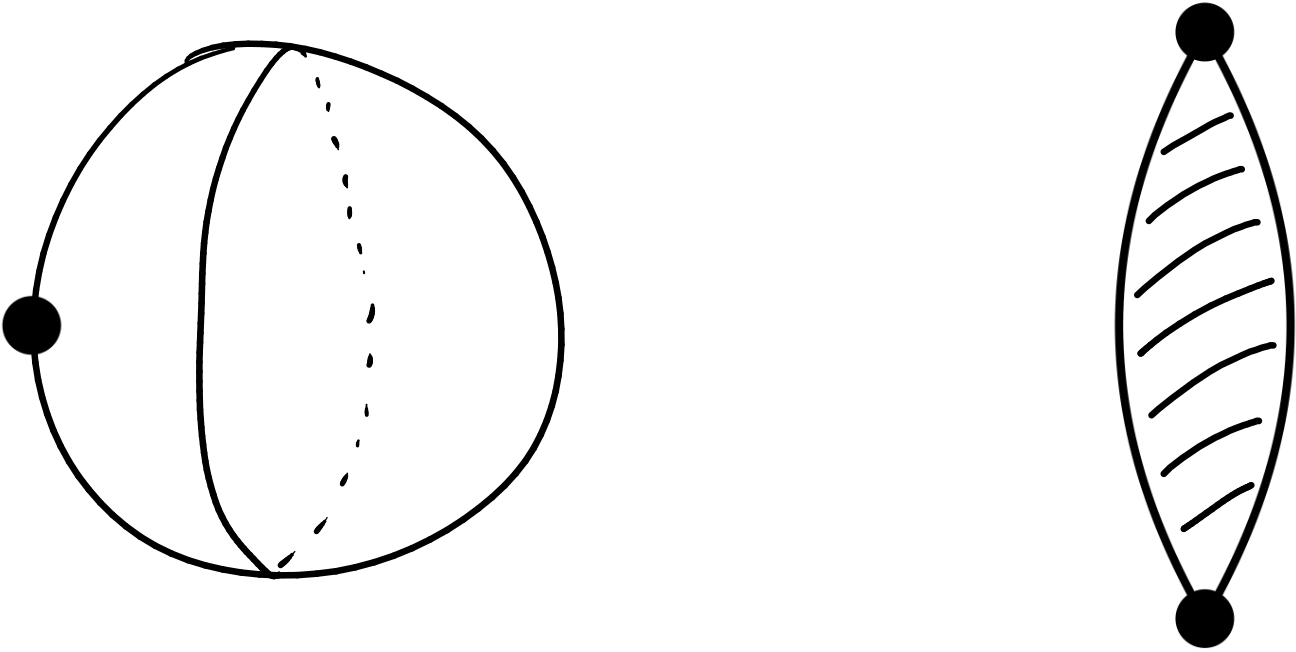
\includegraphics[height=1.2cm]{18_905-201005-1.png}
    \end{tabular}
  \end{center}
  note that attaching a \(k\)-cell (\(k > 1\)) to objects already present
  cannot change the number of path components, which is exactly what the
  proposition says.

  If \(q = 1\), then we have
  \begin{itemize}[nosep]
    \item \(H_1(\Sk_0 X) \iso 0\),
    \item \(H_1(\Sk_1 X)\) is something,
    \item \(H_1(X) \iso H_1(\Sk_2 X) \iso H_1(\Sk_3 X) \iso \cdots\)
  \end{itemize}
  In particular, we have \(H_1(\Sk_1 X) \iso \ZZ\),
  and \(H_1(\Sk_2 X) \iso 0\).
\end{example}

Intuitively, when we add the \(k\)-dimensional cells, we are adding cycles.
But when we compute homologies, we mod out by the boundaries,
which are added when \((k+1)\)-cells are added.
In particular, once \((k+1)\)-cells are added,
higher dimensional cells will not affect \(H_k\).

In general, we have
\begin{itemize}
  \item \(H_q(\Sk_{q-1} X) \iso 0\),
  \item \(H_q(\Sk_q X)\) surjects onto \(H_q(X)\), and
  \item \(H_q(\Sk_{q+1} X) \iso H_q(X)\).
\end{itemize}

\begin{proof}
  To compare \(H_q(\Sk_{k-1} X)\) and \(H_q(\Sk_k X)\),
  we can use the long exact sequence of the pair \((\Sk_k X, \Sk_{k-1} X)\).
  
  The key idea is that
  \[
    H_q(\Sk_k X, \Sk_{k-1} X)
      \iso \tilde H_q \parens{\Sk_k X / \Sk_{k-1} X}
      \iso \tilde H_q \parens[\Big]{\bigvee_{i \in I_k} S^k}
      \iso \begin{cases*}
        \bigoplus_{i \in I_k} \ZZ & if \(q = k\) \\[-1ex]
        0 & otherwise.
      \end{cases*}
  \]
  The long exact sequence of pairs gives
  \(H_q(\Sk_k X) \iso 0\) if \(k < q\)
  because for sufficiently small \(k\), \(H_q(\Sk_k X) \iso H_q(\Sk_{k-1} X)\).
  The long exact sequence also gives
  \(H_q(\Sk_k X) \iso H_q(\Sk_{k+1} X)\) if \(k > q\).
  It remains to check that
  \[
    H_q(\Sk_k X) \simeq H_q(X)
  \]
  if \(k = q\).
  Note that \(\Delta^q\) and \(\Delta^{q+1}\) are compact,
  so anything in \(H_q(X)\) has to be represented by
  a finite linear combination of simplices,
  which by compactness has to be contained in some finite skeleton.
  Knowing \(\Delta^q\) is compact tells us that
  \(H_q(X) \to H_{q+1(X)}\) is surjective,
  and knowing that \(\Delta^{q+1}\) is compact tells us that
  the boundary relations are present as well.
\end{proof}


\section{Cellular homology}
Now we will introduce a tool to compute homology groups.
\begin{definition}
  Suppose \(X\) is a CW complex.
  Let \(C_n(X) = C_n^{\text{cell}}(X)\) denote
  \[
    H_n(\Sk_n X, \Sk_{n-1} X) \simeq
      \tilde H_n \parens[\Big]{\bigvee_{i \in I_n} S^n},
  \]
  the free abelian group on the set of \(n\)-cells of \(X\).
\end{definition}

\begin{definition}
  For each \(n \geq 0\), we can define the map
  \[
    d \colon C_{n+1}(X) \to C_n(X)
  \]
  to be the composite
  \[
    \begin{tikzcd}
      C_{n+1}(X) = H_{n+1}(\Sk_{n+1} X, \Sk_n X) \ar[r, "\partial"] &
      H_n(\Sk_n X) \ar[r] &
      H_n(\Sk_n X, \Sk_{n-1} X) = C_n(X)
    \end{tikzcd}
  \]
\end{definition}

\begin{theorem}
  The maps \(d \colon C_{n+1}(X) \to C_n(X)\) make \(C_*(X)\) into
  a chain complex (i.e.\ \(d \circ d = 0\)).
  The homology of this chain complex is isomorphic to the homology of \(X\).
  This is called \vocab{cellular homology}.
\end{theorem}

Consider the sequence of functors
\[
  \begin{tikzcd}
    \Fun(\Deltainj^\op, \cSet) \ar[r, "F"] &
    \cCWcomp \ar[r, "U"] &
    \cTop
  \end{tikzcd}
\]
i.e.\ the geometric realization of a semisimplicial set.
Then \(C_n^{\text{cell}}(F(X)) = \ZZ \Sing_n X = S_n(X)\)
and \(C_*^{\text{cell}}(F(X)) = S_*(X)\).
Thus, the theorem says that the semisimplicial homology of \(X\) agrees
with the singular homology of the geometric realization of \(X\).

\begin{example}[Homology of \(S^n\)]
  Recall that \(S^n\) has a very simple CW complex structure that requires
  one \(0\)-cell and one \(n\)-cell.
  Since \(C_l^{\text{cell}}(X)\) is the free abelian group on
  the set of \(l\)-cells, we have
  \[
    C_l^{\text{cell}}(S^n) = \begin{cases*}
      \ZZ & if \(l = 0, n\) \\[-1ex]
      0 & otherwise.
    \end{cases*}
  \]

  For e.g.\ \(n = 2\), we have the chain complex \(C_*(S^2)\) is isomorphic to
  \[
    \begin{tikzcd}
      \ZZ &
      0 \ar[l, "d"'] &
      \ZZ \ar[l, "d"'] &
      0 \ar[l, "d"'] &
      0 \ar[l, "d"'] &
      \cdots \ar[l, "d"']
    \end{tikzcd}
  \]
  Since most of these groups are \(0\), we can easily compute:
  \[
    H_0(S^2) \iso \ZZ \qquad
    H_1(S^2) \iso 0 \qquad
    H_2(S^2) \iso \ZZ \qquad
    H_3(S^2) \iso 0,
  \]
  i.e.\ \(H_q(S^2) \iso \begin{cases*}
    \ZZ & if \(q = 0, 2\) \\[-1ex]
    0 & otherwise.
  \end{cases*}\)
\end{example}

\begin{remark}
  If a CW complex only has even dimensional cells, then
  \[
    H_q(X) \iso \begin{cases*}
      \bigoplus_{i \in I_q} \ZZ & \(q\) is even \\[-1ex]
      0 & \(q\) is odd.
    \end{cases*}
  \]
\end{remark}

\begin{example}[Torus]<torus-cell-homology>
  The torus \(T^2\) has a CW structure
  \begin{align*}
    \Sk_0 T^2 &= * \\[-1ex]
    \Sk_1 T^2 &= \enskip 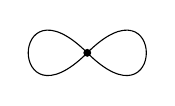
\begin{tikzpicture}[baseline, yshift=0.6ex]
      \fill (0, 0) circle (0.05);
      \draw (0, 0) .. controls (1/4, -1/4) and (7/16, -5/16) .. (9/16, -9/32);
      \draw (9/16, -9/32) .. controls (11/16, -1/4) and (3/4, -1/8) .. (3/4, 0);
      \draw (3/4, 0) .. controls (3/4, 1/8) and (11/16, 1/4) .. (9/16, 9/32);
      \draw (9/16, 9/32) .. controls (7/16, 5/16) and (1/4, 1/4) .. (0, 0);
      \begin{scope}[xscale=-1]
        \draw (0, 0) .. controls (1/4, -1/4) and (7/16, -5/16) .. (9/16, -9/32);
        \draw (9/16, -9/32) .. controls (11/16, -1/4) and (3/4, -1/8) .. (3/4, 0);
        \draw (3/4, 0) .. controls (3/4, 1/8) and (11/16, 1/4) .. (9/16, 9/32);
        \draw (9/16, 9/32) .. controls (7/16, 5/16) and (1/4, 1/4) .. (0, 0);
      \end{scope}
    \end{tikzpicture}
    \enskip = 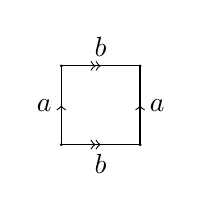
\begin{tikzpicture}[baseline, yshift=-3.4ex]
      \begin{scope}[decoration={markings, mark=at position 0.5 with {\arrow{>>}}}]
        \draw[postaction={decorate}] (0, 0) -- (1, 0) node[midway, below]{\(b\)};
        \draw[postaction={decorate}] (0, 1) -- (1, 1) node[midway, above]{\(b\)};
      \end{scope}
      \begin{scope}[decoration={markings, mark=at position 0.5 with {\arrow{>}}}]
        \draw[postaction={decorate}] (1, 0) -- (1, 1) node[midway, right]{\(a\)};
        \draw[postaction={decorate}] (0, 0) -- (0, 1) node[midway, left ]{\(a\)};
      \end{scope}
      \fill (0, 0) circle[radius=0.02];
      \fill (0, 1) circle[radius=0.02];
      \fill (1, 0) circle[radius=0.02];
      \fill (1, 1) circle[radius=0.02];
    \end{tikzpicture} \\ % chktex 31
    \Sk_2 T^2 &= \enskip\parbox{0.15\textwidth}{%
      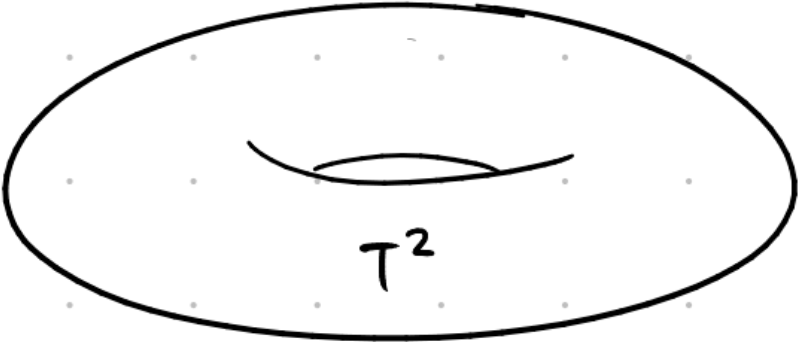
\includegraphics[width=0.15\textwidth]{18_905-201005-2-torus.png}}
  \end{align*}
  where the \(2\)-skeleton is obtained by attaching one \(2\)-cell
  via the map \(S^1 \to \Sk_1 T^2\) which is \(b\inv a\inv b a\).

  We can compute the homology group from the cellular chain complex
  \[
    \begin{tikzcd}
      \ZZ\fgen{x} &
      \ZZ\fgen{a, b} \iso \ZZ \oplus \ZZ \ar[l, "d_1"'] &
      \ZZ\fgen{u} \ar[l, "d_2"'] &
      0 \ar[l] &
      \cdots \ar[l]
    \end{tikzcd}
  \]
  Note that \(d_1\) has to be zero because the boundaries
  of \(a\) and \(b\) are the same point.
  To compute \(d_2\), note that the boundary of the \(2\)-cell \(u\)
  is glued on via \(b\inv a\inv b a\).
  Therefore,
  \[
    d_2 u = -b -a + b + a = 0.
  \]
  This gives the expected homology groups.
\end{example}

\begin{proof}[\(C_*^{\text{cell}}(X)\) agrees with singular homology]
  Consider the diagram
  \[
    \begin{tikzcd}
      & \mathllap{C_{n+1}^{\text{cell}}(X) = {}}
        H_{n+1}(\Sk_{n+1} X, \Sk_n X) \ar[d, blue, "\partial_n"] \ar[dr, "d"]
        & & H_{n-1}(\Sk_{n-2} X) \mathrlap{{} = 0} \ar[d] \\
      \mathllap{0 = {}} H_{n+1}(\Sk_{n-1} X) \ar[r]
        & H_n(\Sk_n X) \ar[r, blue, "j_n"] \ar[d]
        & H_n(\Sk_n X, \Sk_{n-1} X) \ar[r, blue, "\partial_{n-1}"] \ar[dr, "d"]
        & H_{n-1}(\Sk_{n-1} X) \ar[d, blue, "j_{n-1}"] \\
      & H_n(\Sk_{n+1} X) \ar[d]
        & & H_{n-1}(\Sk_{n-1} X, \Sk_{n-2} X) \\
      & \mathllap{0 = {}} H_n(\Sk_{n+1} X, \Sk_n X)
    \end{tikzcd}
  \]
  All of the rows and columns are exact.
  The theorem claims that \(d \circ d = 0\),
  and \(\ker d / \img d\) agrees with singular homology.

  To show that \(d \circ d = 0\), note that \(d \circ d\) is the same as
  following the blue arrows. However, the horizontal sequence is exact, so
  the composite of the two blue horizontal maps is zero.

  To show that \(\ker d / \img d\) computes singular homology,
  note that \(j_{n-1}\) is injective from exactness. Therefore,
  \(\ker d = \ker \partial_{n-1}\),
  and furthermore
  \(\ker d = \ker \partial_{n-1} = \img j_n\)
  by exactness of the horizontal sequence.
  We also have \(j_n\) is injective from exactness,
  so \(\img j_n \iso H_n(\Sk_n X)\).

  Therefore,
  \[
    \frac{\ker d}{\img d}
      = \frac{H_n(\Sk_n X)}{\img \partial_n}
      = H_n(\Sk_{n+1} X)
      = H_n(X). \pog
  \]
\end{proof}




\end{document}

\documentclass{standalone}
\usepackage{chez}

\begin{document}
\chapter{October 07, 2020}

Last time we saw that the cellular chain complex \(C_*^{\text{cell}}(X)\) of
a CW complex \(X\) computes the singular homology.

\begin{example}[\(S^2\)]
  Let's consider a less-minimal cell structure of \(S^2\) where
  \[
    \Sk_0 S^2 = S^0 \qquad
    \Sk_1 S^2 = S^1 \qquad
    \Sk_2 S^2 = S^2,
  \]
  depicted below.
  \begin{center}
    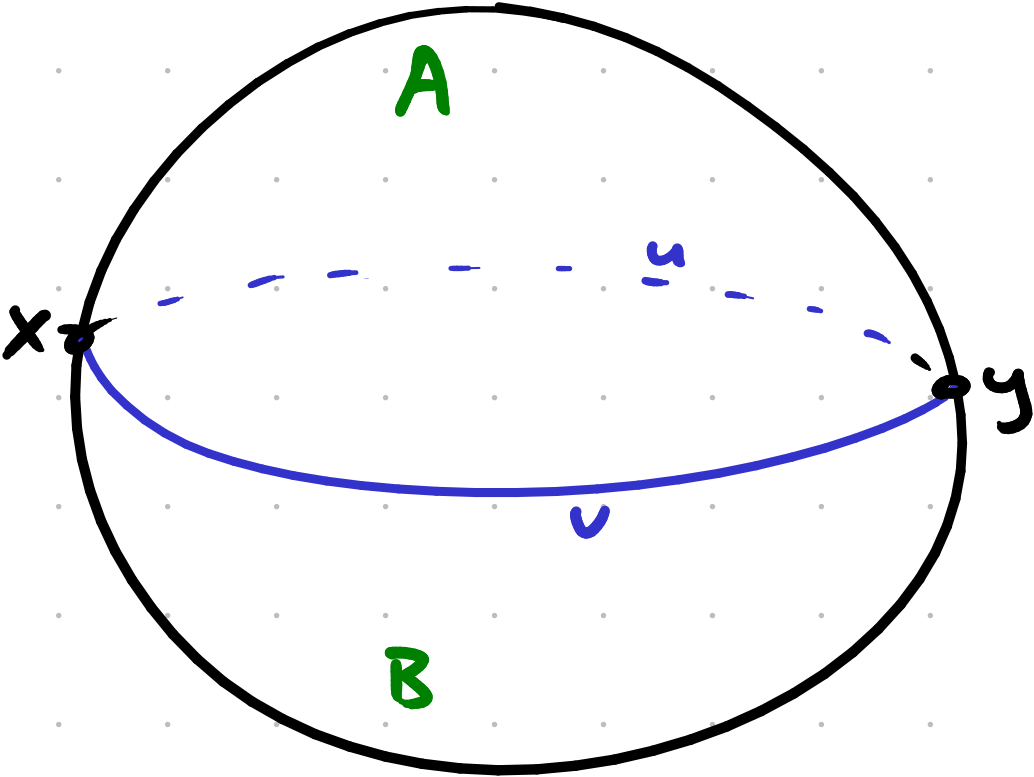
\includegraphics[width=0.2\textwidth]{18_905-201007-1.png}
  \end{center}
  Then
  \[
    C_*^{\text{cell}}(S^2) = \Big({
      \begin{tikzcd}
      	\ZZ\fgen{x, y} &
      	\ZZ\fgen{u, v} \ar[l, "d"'] &
      	\ZZ\fgen{A, B} \ar[l, "d"'] &
      	\cdots \ar[l]
      \end{tikzcd}
    }\Big)
  \]
  Note that when we are computing the homology maps,
  we only care about the image of the \(d\) maps.
  In particular, when we are working with semisimplicial sets,
  we cared about the direction that the edges went.
  Here we can make an arbitrary choice of direction to help us
  compute the \(d\) maps.
  In particular, if we select \(x \overset{u}\to y\)
  and \(x \overset{v}\to y\), then
  \[
    du = y - x, \qquad dv = y - x.
  \]
  Then
  \[
    H_0(S^2) = \frac{\ker d}{\img d} = \frac{\ZZ\fgen{x, y}}{\ZZ\fgen{y - x}}
      \iso \ZZ.
  \]

  To determine \(dA\) and \(dB\), note that we can add some maps
  to the pushout diagram of the \(2\)-skeleton
  \[
    \begin{tikzcd}
      S^1 \sqcup S^1 \arrow[r, "f"] \arrow[d, hook] &
        \Sk_1 S^2 \mathrlap{{} = S^1} \arrow[d] \\
      D^2 \sqcup D^2 \arrow[r] &
        \Sk_2 S^2 \mathrlap{{} = S^2}
    \end{tikzcd}
  \]
  Note that the map \(f\) determines \(\Sk_2 S^2\) as the pushout.
  In particular, consider the map
  \[
    \begin{tikzcd}
      S^1 \sqcup S^1 \ar[r] &
    	\Sk_1 S^2 \ar[r] &
    	\Sk_1 S^2 / \Sk_0 S^2 = S^1 \vee S^1
    \end{tikzcd}
  \]
  Taking \(H_1\), this gives a map
  \[
    \ZZ \oplus \ZZ \to \ZZ \oplus \ZZ
  \]
  that gives the information of \(dA\) and \(dB\),
  since the \(\ZZ\)s on the left represent \(A\) and \(B\),
  and the \(\ZZ\)s on the right represent \(u\) and \(v\).

  In particular, we can again arbitrarily assign
  \[
    dA = u - v, \qquad
    dB = u - v.
  \]
  And indeed, when we compute the homologies from this sequence,
  we get the expected result.

  Moreover, we have that a generator of \(H_2(S^2)\)
  in this CW structure is given by \(A - B\).
  This is because we know \(dA = dB\), since the attaching maps
  \(S^1 \to \Sk_1 S^1\) defining \(A\) and \(B\) are the same.
\end{example}

\subsection{Homotopy equivalence}
Note that homology can be used to prove that topological spaces
are not homotopy equivalent.
In particular, this is just a consequence of homology
being an invariant under homology.

A less obvious statement is that homology can also be used
to prove that continuous maps are not homotopic.
Homology is a functor, so it takes maps in \(\cTop\) to maps in \(\cAb\).
So, if two continuous maps are sent to different maps of abelian groups,
then the two continuous maps cannot be homotopic.

\begin{definition}
  If \(f \colon S^n \to S^n\) is a continuous map,
  then the \vocab{degree} of \(f\), denoted \(\deg f\), is the value of \(1\)
  under the group homomorphism \(H_n(f) \colon \ZZ \to \ZZ\).
\end{definition}

If \(f, g \colon S^n \to S^n\) are two continuous maps that
have different degrees, then \(f\) and \(g\) are hot homotopic,
as otherwise \(H_n(f) = H_n(g)\).

\begin{lemma}
  Suppose \(f, g \colon S^n \to S^n\). Then
  \[
    \deg (g \circ f) = (\deg g)(\deg f).
  \]
\end{lemma}
\begin{proof}
  Consider the diagram
  \[
    \begin{tikzcd}
    	S^n \ar[r, "f"] &
    	S^n \ar[r, "g"] &
    	S^n
    \end{tikzcd}
  \]
  When we apply \(H_n\), we get
  \[
    \begin{tikzcd}[row sep=0.15]
      \ZZ \ar[r, "H_n(f)"] &
        \ZZ \ar[r, "H_n(g)"] &
        \ZZ \\
      1 \ar[r, mapsto] & \deg f \\
      & 1 \ar[r, mapsto] & \deg g \\
      1 \ar[rr, mapsto] & & (\deg f)(\deg g)
    \end{tikzcd}
  \]
\end{proof}

\begin{corollary}
  Suppose \(f \colon S^n \to S^n\) is a homeomorphism.
  Then \(\deg f\) is either \(1\) or \(-1\).
\end{corollary}

\begin{example}
  Consider the map \(f \colon S^2 \to S^2\) that is
  a reflection about a plane.
  Note that \(f\) is also a map of CW complexes.
  If we select the skeleta such that the plane of reflection is the equator,
  then we know that \(A\) and \(B\) have the same boundary, and the map
  \[
    S^1 \sqcup S^1 \to \Sk_1 S^2 \to \Sk_1 S^2 / \Sk_0 S^2 \iso S^1 \vee S^1
  \]
  sends the boundaries of \(A\) and \(B\) to the same set.
  In particular, we know that \(d A = d B\), so
  \[
    A - B \in \ker d = H_2^{\text{cell}}(S^2) \iso \ZZ.
  \]
  Therefore, \(A - B\) is a generator of \(H_2^{\text{cell}}(S^2)\).
  In particular, \(f\) is the map between the cellular complexes
  \[
    \begin{tikzcd}
      \ZZ\fgen{A, B} \arrow[r]
        \arrow[d, "A \mapsto B" pos=0.2, "B \mapsto A" pos=0.6] &
        \ZZ\fgen{u, v} \arrow[r]
          \arrow[d, "u \mapsto u" pos=0.2, "v \mapsto v" pos=0.6] &
        \ZZ\fgen{x, y}
          \arrow[d, "x \mapsto x" pos=0.2, "y \mapsto y" pos=0.6] \\
      \ZZ\fgen{A, B} \arrow[r] &
        \ZZ\fgen{u, v} \arrow[r] &
        \ZZ\fgen{x, y}
    \end{tikzcd}
  \]
  This means \(f \colon A - B \mapsto B - A\),
  so \(H_2(f) \colon \ZZ \to \ZZ\) is multiplication by \(-1\).
  Therefore, \(f\) has degree \(-1\).
\end{example}
Note that this argument also works for \(S^n\) in general,
so no reflection \(S^n \to S^n\) is homotopic to the identity.

\begin{corollary}
  The degree of a rotation of \(S^n\) is \(1\).
\end{corollary}
This is because any rotation can be written as
the composition of two reflections.

\begin{example}
  \begin{itemize}[nosep]
    \item The degree of \(S.to S^1\) where \(x \mapsto -x\) is \(1\) because
          it is a \(180^\circ\) rotation.
    \item We can find he degree of \(S^2 \to S^2\) where \(x \mapsto -x\)
          by considering the map as the composite of three reflections
          \[
            (a, b, c) \mapsto (-a, b, c)
                      \mapsto (-a, -b, c)
                      \mapsto (-a, -b, -c).
          \]
          Therefore, this map has degree \(-1\).
    \item More generally, the antipodal map \(S^n \to S^n\)
          mapping \(x \mapsto -x\) is the composite of \(n+1\) reflections,
          so the map has degree \((-1)^{n+1}\).
  \end{itemize}
\end{example}





\end{document}

\documentclass{standalone}
\usepackage{chez}

\begin{document}
\chapter{October 09, 2020}

\subsection{Summary}
If \(X\) is a CW complex, then \(\Ccell_*(X)\) is a chain complex
with homology groups computing the singular homology groups \(H_q(X)\).
The \(n\)th group \(\Ccell_n(X)\) is the free abelian group on the
set \(I_n\) of \(n\)-cells. To compute the differential
\(d \colon \Ccell_n(X) \to \Ccell_{n-1}(X)\),
we consider the diagram
\[
  \begin{tikzcd}
    \coprod_{i \in I_n} S^{n-1} \arrow[r] \arrow[d] &
      \Sk_{n-1} X \arrow[d] \arrow[r] &
      \Sk_{n-1} X / \Sk_{n-2} X
        \mathrlap{{} \iso \bigvee_{i \in I_{n-1}} S^{n-1}} \\
    \coprod_{i \in I_n} D^n \arrow[r] &
       \Sk_n X
  \end{tikzcd}
\]
Applying \(H_{n-1}\) to the top row,
\(d \colon \Ccell_n(X) \to \Ccell_{n-1}(X)\).

If \(f \colon X \to Y\) is a map in \(\cTop\),
then to compute \(H_q(f) \colon H_q(X) \to H_q(Y)\),
We can place CW structures on \(X\) and \(Y\) so that
\(f\) induces a map \(\Ccell_*(X) \to \Ccell_*(Y)\).

\subsection{Homology of real projective space}
Recall \(\RP^n \coloneq S^n / (x \sim -x)\).
To compute the homology of this, we may try to do this by
coming up with a semisimplicial model for this space,
but it is not obvious how to do this.

However, we do have a CW structure on \(\RP^n\),
with one \(k\)-cell in each dimension \(0 \leq k \leq n\).
We can try to determine \(H_q(\RP^2)\).
Consider the pushout square
\[
  \begin{tikzcd}[row sep=small]
    S^1 \arrow[r] \arrow[d] &
      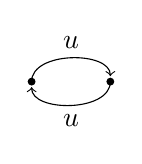
\begin{tikzpicture}[yshift=0.6ex]
        \fill (-1/2, 0) circle (0.05);
        \fill (1/2, 0) circle (0.05);
        \path[->, shorten >=2] (-1/2, 0) edge[in=90, out=90] node[above] {\(u\)} (1/2, 0);
        \path[<-, shorten <=2] (-1/2, 0) edge[in=-90, out=-90] node[below] {\(u\)} (1/2, 0);
      \end{tikzpicture} \arrow[d] \arrow[r, "\text{quotient}"] &
      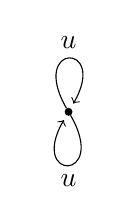
\begin{tikzpicture}
        \fill (0, 0) circle (0.05);
        \path[->, shorten >=2] (120: 0.05) edge[in=60, out=120, looseness=50] node[above] {\(u\)} (60: 0.05);
        \path[->, shorten >=2] (-60: 0.05) edge[in=-120, out=-60, looseness=50] node[below] {\(u\)} (-120: 0.05);
      \end{tikzpicture}
      \mathrlap{{} \iso S^1} \\
    D^2 \arrow[r] &
      \RP^2
  \end{tikzcd}
\]
Taking \(H_1\) of the top row, we have a map \(\ZZ \to \ZZ\).
More specifically, the \(2\)-cell gets mapped to \(u^2\),
so the map is \(1 \mapsto 2\).
We have the chain \(\Ccell_*(\RP^2)\)
\[
   \begin{tikzcd}[row sep=0.2]
  	0 \ar[r] &
      \ZZ\fgen{A} \ar[r] &
      \ZZ\fgen{u} \ar[r] &
      \ZZ\fgen{x} \\
    & A \ar[r, mapsto] &
      2u \\
    & & u \ar[r, mapsto] &
      0
  \end{tikzcd}
\]
This gives
\[
  H_0(\RP^2) \iso \ZZ, \qquad
  H_1(\RP^2) \iso \ZZ / 2\ZZ, \qquad
  H_2(\RP^2) \iso 0.
\]
This is a bit weird. Usually our homologies are free abelian groups.
Here, this means that there is some loop that is not a boundary,
but when we go around it twice, it is a boundary.

Now let's consider \(\Ccell_*(\RP^n)\) in general.
Let's try to think about this inductively.
If we understand \(\Ccell_*(\RP^{n-1})\),
can we say anything about \(\Ccell_*(\RP^{n})\)?
Consider the pushout diagram
\[
  \begin{tikzcd}
    S^{n-1} \arrow[r] \arrow[d] &
      \RP^{n-1} \arrow[d] \arrow[r] &
      \RP^{n-1} / \RP^{n-2} \mathrlap{{} \iso S^{n-1}} \\
    D^n \arrow[r] &
      \RP^n
  \end{tikzcd}
\]
Note that the way that we can think about \(\RP^{n-1} / \RP^{n-2}\)
is to take \(S^{n-1} \vee S^{n-1}\) and quotient by the antipodal map
between the two spheres.
The differential \(d\) maps \(1\) to \(1 + \deg f\),
where \(f\) is antipodal map \(S^{n-1} \to S^{n-1}\).
This is because the top half of the first \(S^{n-1}\)
gets mapped to \(S^{n-1}\), and the bottom half
gets mapped to the second \(S^{n-1}\), but under the quotient
this is equal to the antipodal map of the identity.
Therefore, \(d \colon 1 \mapsto 1 + (-1)^n\).

This gives the chain
\[
  \Ccell_*(\RP^n) \iso \Big(
  \begin{tikzcd}
  	\cdots \ar[r] &
  	0 \ar[r] &
  	\ZZ \ar[r] &
  	\cdots \ar[r] &
  	\ZZ \ar[r, "2"] &
  	\ZZ \ar[r, "0"] &
  	\ZZ \ar[r, "2"] &
  	\ZZ \ar[r, "0"] &
  	\ZZ
  \end{tikzcd}
  \Big),
\]
where the number of \(\ZZ\)s in the chain is \(n+1\).
In general, this means for even \(n\),
\[
  H_q(\RP^n) = \begin{cases*}
    \ZZ & \(q = 0\) \\[-1ex]
    \ZZ/2\ZZ & \(0 < q < n\), odd \(q\) \\[-1ex]
    0 & otherwise
  \end{cases*}
\]
and for odd \(n\),
\[
  H_q(\RP^n) = \begin{cases*}
    \ZZ & \(q = 0, n\) \\[-1ex]
    \ZZ/2\ZZ & \(0 < q < n\), odd \(q\) \\[-1ex]
    0 & otherwise.
  \end{cases*}
\]

\section{Other invariants}
Let's talk about other invariants that give strictly less information
than homology. The advantage is that they are easier to compute than homology.

\begin{definition}
  If \(X\) is a finite CW complex,
  then the \vocab{Euler characteristic} is
  \[
    \chi(X) = \sum_k (-1)^k \size{I_k}.
  \]
\end{definition}

\begin{example}
  Consider \(S^2\) with one \(0\)-cell and one \(2\)-cell.
  The Euler characteristic is \(\chi(S^2) = 1 + 1 = 2\).

  There is the other CW structure with two \(0\)-cells,
  \(1\)-cells, and \(2\)-cells.
  This gives the Euler characteristic \(\chi(S^2) = 2 - 2 + 2 = 2\).
\end{example}

\begin{theorem}
  The Euler characteristic \(\chi(X)\) depends only on
  the homotopy type of \(X\).
\end{theorem}

\begin{example}
  Consider the torus \(T^2\) with the CW structure
  from \cref{ex:torus-cell-homology}.
  This gives us the Euler characteristic
  \(\chi(T^2) = 1 - 2 + 1 = 0\).

  A corollary of this is that \(T^2\) and \(S^2\)
  are not homotopy equivalent.
\end{example}

\begin{theorem}
  If \(X\) is a finite CW complex, then
  \[
    \chi(X) = \sum_k (-1)^k \rank H_k(X).
  \]
\end{theorem}
To define rank, recall that abelian groups are equivalent to \(\ZZ\)-modules.
Since \(\ZZ\) is a PID, there is a classification of finitely generated
abelian groups. In particular, every finitely generated abelian group \(A\)
is isomorphic to
\[
  \ZZ^r \oplus \ZZ/n_1\ZZ \oplus \dots \oplus \ZZ/n_t\ZZ
\]
where \(r \geq 0\) and \(n_1, \dots, n_t \geq 2\).
We call \(r\) the \vocab{rank} of \(A\).

Note that since \(X\) is a finite CW complex, we know that \(H_k(X)\)
is finitely generated for each \(k\).







\end{document}

\documentclass{standalone}
\usepackage{chez}

\begin{document}
\chapter{October 13, 2020}

\begin{lemma}
  Let
  \[
    \begin{tikzcd}
      0 \ar[r] &
      A \ar[r] &
      B \ar[r] &
      C \ar[r] &
      0
    \end{tikzcd}
  \]
  be a short exact sequence of finitely generated abelian groups.
  Then \(\rank B = \rank A + \rank C\).
\end{lemma}
We will prove a variant of this on the problem set.

Now we can prove \(\chi(X) = \sum_k (-1)^k \rank H_k(X)\).
\begin{proof}
  Consider, for all \(k \geq 0\), there are short exact sequences
  \[
    \begin{tikzcd}
      0 \ar[r] &
      Z^{\text{cell}}_k(X) \ar[r] &
      \Ccell_k(X) \ar[r, "\partial"] &
      B^{\text{cell}}_{k-1}(X) \ar[r] &
      0
    \end{tikzcd}
  \]
  Indeed, it is exact at \(Z^{\text{cell}}_k(X)\) because the map
  \(Z^{\text{cell}}_k(X) \to C^{\text{cell}}_k(X)\) is injective, since the cycles of \(X\) are
  a subset of the chains of \(X\).
  Moreover, it is exact at \(C^{\text{cell}}_k(X)\) because the
  chains are precisely the elements in kernel of the boundary map \(\partial\).
  Then, the boundaries are defined do be the image of the boundary map,
  so \(\partial\) is surjective and the sequence is exact at
  \(B^{\text{cell}}_{k-1}(X)\).

  There is another short exact sequence
  \[
    \begin{tikzcd}
      0 \ar[r] &
      B^{\text{cell}}_k(X) \ar[r] &
      Z^{\text{cell}}_k(X) \ar[r] &
      H_k(X) \ar[r] &
      0
    \end{tikzcd}
  \]
  It's exact at \(B^{\text{cell}}_k(X)\) because
  \(B^{\text{cell}}_k(X) \to Z^{\text{cell}}_k(X)\) is an injection,
  which is equivalent to the fact that every boundary is a cycle,
  i.e.\ \(\partial^2 = 0\).
  Also, we know that \(H_k(X)\) is the quotient of \(Z^{\text{cell}}_k(X)\)
  by \(B^{\text{cell}}_k(X)\) by definition, so the sequence
  is exact at \(Z^{\text{cell}}_k(X)\) and \(H_k(X)\).

  Using these short exact sequences, we know
  \begin{align*}
    \sum_k (-1)^k \size{I_k}
      &= \sum_k (-1)^k \rank (C^{\text{cell}}_k(X)) \\
      &= \sum_k (-1)^k (
        \rank (Z^{\text{cell}}_k(X)) + \rank (B^{\text{cell}}_{k-1}(X))
      ) \\
      &= \sum_k (-1)^k (
        \rank (B^{\text{cell}}_k(X))
        + \rank (H_k(X))
        + \rank (B^{\text{cell}}_{k-1}(X))
      ).
  \intertext{Note that the \(B^{\text{cell}}_k(X)\) terms telescope, so}
      &= \sum_k (-1)^k (\rank (H_k(X))). \pog
  \end{align*}
\end{proof}

\section{Homology with coefficients}
Another invariant easier to compute than homology is
\vocab{homology with coefficients}.
When defining homology, we applied the free abelian group functor
on the simplices of a semisimplicial set.
But one does not need to use this specific functor.
There are other functors that we can choose.
\begin{definition}
  Let \(R\) be a commutative ring and \(X\) be a semisimplicial set.
  For any \(k \geq 0\), let \(S_k(X; R)\),
  read ``\(S_k\) of \(X\) with coefficients in \(R\)'',
  to be the free \(R\)-module generated by \(X_k\).

  Let \(R\) be a commutative ring and \(X\) be a topological space.
  We can similarly define \(S_k(X, R)\) to be the free \(R\)-module
  generated by \(\Sing_k(X)\).
\end{definition}
Note that \(S_k(X, \ZZ) = S_k(X)\) because \(\ZZ\)-modules are
the same thing as abelian groups.

In both cases, whether we're dealing with semisimplicial sets
or topological spaces, the alternating sum of the semisimplicial face maps
creates the differential in a chain complex \(S_k(X; R)\).
In particular, the chain complex is of \(R\)-modules where
the differentials are \(R\)-module maps.

\begin{example}
  Consider the following semisimplicial set:
  \begin{center}
    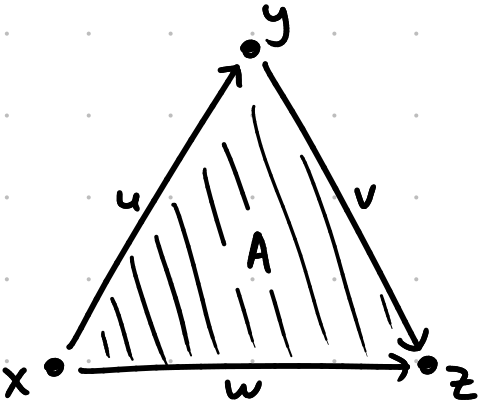
\includegraphics[width=0.2\textwidth]{18_905-201013-1.png}
  \end{center}
  Then \(S_*(X; \QQ)\) is a chain complex of rational vector spaces
  and linear maps isomorphic to
  \[
    \begin{tikzcd}
      \cdots \ar[r] &
      0 \ar[r] &
      \QQ \ar[r] &
      \QQ \oplus \QQ \oplus \QQ \ar[r] &
      \QQ \ar[r] &
      0 \ar[r] &
      \cdots
    \end{tikzcd}
  \]
  where the nonzero vector spaces have bases \(\set{A}\), \(\set{u, v, w}\),
  and \(\set{x, y, z}\) respectively.
  The maps are the maps that we expect
  \[
    \begin{aligned}[t]
      \QQ & \to \QQ \oplus \QQ \oplus \QQ \\[-1ex]
      A &\mapsto u + v - w
    \end{aligned}
    \qquad
    \begin{aligned}[t]
      \QQ \oplus \QQ \oplus \QQ & \to \QQ \\[-1ex]
      u &\mapsto y - x \\[-1ex]
      v &\mapsto z - y \\[-1ex]
      w &\mapsto z - x.
    \end{aligned}
  \]
\end{example}

The homology \(R\)-modules of \(S_*(X; R)\) are denoted by \(H_q(X; R)\).
Homology with coefficients in a commutative ring satisfies all of
the Eilenberg-Steenrod axioms where the dimension axiom is modified to say
\[
  H_q(*; R) = \begin{cases*}
    R & if \(q = 0\) \\[-1ex]
    0 & otherwise.
  \end{cases*}
\]

All of the theory we've built up to calculate homology works with
homology with coefficients, so if \(X\) is a CW complex,
we can also calculate \(H_q(X; R)\) using the cellular chain complex
\(C^{\text{cell}}_*(X; R)\).

\begin{example}
  Let's consider \(\RP^2\) with the CW structure with
    one \(0\)-cell,
    one \(1\)-cell, and
    one \(2\)-cell.
  We calculated \(H_q(\RP^2) = H_q(\RP^2; \ZZ)\) with the
  cellular chain complex
  \[
    \begin{tikzcd}
      \cdots \ar[r] &
      0 \ar[r] &
      \ZZ \ar[r, "2"] &
      \ZZ \ar[r, "0"] &
      \ZZ \ar[r] &
      0 \ar[r] &
      \cdots
    \end{tikzcd}
  \]
  In particular we calculated
  \[
    H_q(\RP^2) = \begin{cases*}
      \ZZ & if \(q = 0\) \\[-1ex]
      \ZZ/2\ZZ & if \(q = 1\) \\[-1ex] % chktex 1
      0 & otherwise.
    \end{cases*}
  \]
  We can also calculate \(H_q(\RP^2; \QQ)\) with the cellular chain complex
  \[
    \begin{tikzcd}
      \cdots \ar[r] &
      0 \ar[r] &
      \QQ \ar[r, "2"] &
      \QQ \ar[r, "0"] &
      \QQ \ar[r] &
      0 \ar[r] &
      \cdots
    \end{tikzcd}
  \]
  Then we have the homology
  \[
    H_q(\RP^2) = \begin{cases*}
      \QQ & if \(q = 0\) \\[-1ex]
      \ZZ/2\ZZ \iso 0 & if \(q = 1\) \\[-1ex] % chktex 1
      0 & otherwise.
    \end{cases*}
  \]
  We can also calculate \(H_q(\RP^2; \FF_2)\). We have the chain
  \[
    \begin{tikzcd}
      \cdots \ar[r] &
      0 \ar[r] &
      \FF_2 \ar[r, "2"] &
      \FF_2 \ar[r, "0"] &
      \FF_2 \ar[r] &
      0 \ar[r] &
      \cdots
    \end{tikzcd}
  \]
  This gives the homology
  \[
    H_q(\RP^2; \FF_2) = \begin{cases*}
      \FF_2 & if \(q = 0, 1, 2\) \\[-1ex]
      0 & otherwise.
    \end{cases*}
  \]
\end{example}

\begin{note}
  All subsequent material will not be tested until after November 9th.
\end{note}

We have covered the main ideas of homology.
However, there are more things we can ask about.
\begin{question}
  In what sense is \(H_q(X; R)\) easier than \(H_q(X; \ZZ)\)?
  Is \(H_q(X; R)\) determined by \(H_q(X; \ZZ)\)?
\end{question}
It turns out that the answer to the second question is yes.

\begin{note}
  In applied topology, one is given a giant collection of points in,
  e.g.\ \(\RR^{100}\).
  Fix a radius \(R\) and connect any two points within \(R\) of each other,
  draw a \(2\)-simplex for any three points which are
    within some diameter \(R\) circle, etc.
  We get a simplicial complex.
  We can compute the homology, and it turns out that using \(\QQ\) coefficients
  as opposed to \(\ZZ\) has much lower computational complexity.
\end{note}

\begin{question}
  How do we compute \(H_q(X \times Y)\) in terms of \(H_q(X)\) and \(H_q(Y)\)?
\end{question}

\begin{question}
  A topological space \(X\) has a diagonal map
  \(\Delta \colon X \to X \times X\) mapping \(x \mapsto (X, X)\).
  What can we say about \(H_q(\Delta X)\)?
\end{question}

\begin{question}
  What special features are enjoyed by the homology groups of manifolds
  as opposed to generic topological spaces?
\end{question}

On the way to answering these questions,
we will introduce the purely algebraic functors \(\Tor\), \(\Ext\),
and cohomology.





\end{document}

\documentclass{standalone}
\usepackage{chez}

\begin{document}
\chapter{October 14, 2020}

\section{Some algebra}
If \(A\) and \(B\) are abelian groups,
and \(f, g \colon A \to B \in \Hom_{\cAb}(A, B)\),
we can compute \(f + g\) and \(f - g\).
Therefore, we can make the set \(\Hom_{\cAb}(A, B)\) into an abelian group,
denoted \(\ul{\Hom}_\cAb(A, B)\).

More generally, if \(R\) is a commutative ring and \(\cRmod\) is
the category of \(R\)-modules, then \(\Hom_\cRmod(M, N)\) can be
given the structure of an \(R\)-module.
We denote this \(R\)-module \(\underline{\Hom}_\cRmod(M, N)\).

\begin{example}
  Linear maps between two vector spaces over a field form a vector space.
\end{example}

This construction \((M, N) \mapsto \ul\Hom_{\cRmod}(M, N)\) is functorial,
i.e.\ it is natural in its inputs. More specifically,
\begin{enumerate}
  \item If \(N \to N'\) is a map of \(R\)-modules, then any map \(M \to N\)
        gives a composite map \(M \to N \to N'\). There is a \(R\)-module map
        \(\ul\Hom_\cRmod(M, N) \to \ul\Hom_\cRmod(M, N')\).
  \item If \(M \to M'\) is an \(R\)-module map, then there is a corresponding
        map, for every \(N\),
        \(\ul\Hom_\cRmod(M', N) \to \ul\Hom_\cRmod(M, N)\).
\end{enumerate}
Note that in the first map, it goes from \(N\) to \(N'\),
and in the second map, it goes from \(M'\) to \(M\).
We can summarize this by saying that there is a functor
\begin{align*}
  \ul\Hom_\cRmod \colon& (\cRmod)^\op \times (\cRmod) \to \cRmod \\[-1ex]
    & (M, N) \mapsto \ul\Hom_\cRmod(M, N)
\end{align*}

Some categories \(\mathcal C\), like \(\cRmod\), have \vocab{internal Hom}s,
which are functors
\[
  \ul\Hom_{\mathcal C} \colon \mathcal C^\op \times \mathcal C \to \mathcal C.
\]
Here, \(\mathcal C^\op \times \mathcal C\) refers to the product category
of \(\mathcal C^\op\) and \(\mathcal C\) in \(\cCat\).

For example, the category \(\cSet\) has an internal \(\Hom\) with
\[
  \ul\Hom_\cSet(A, B) = \Hom_\cSet(A, B).
\]

If \(A, B, C \in \cSet\) there is a \vocab{currying isomorphism}
\[
  \Hom_\cSet(A \times B, C) \iso \Hom_\cSet(A, \Hom_\cSet(B, C))
\]
where a function \(f \colon A \to \Hom_\cSet(B, C)\) is sent to the function
\(g \colon A \times B \to C\) given by
\[
  g(a, b) = (f(a))(b).
\]
Whenever there is an internal \(\Hom\), there is generally a isomorphism
of this flavor.
The analog of the currying isomorphism in \(\cRmod\) is the following:
\begin{theorem}
  Let \(R\) be a commutative ring.
  There is a functor \vocab{tensor product}
  \[
    \otimes_R \colon \cRmod \times \cRmod \to \cRmod
  \]
  such that
  \[
    \ul\Hom_\cRmod(A \otimes_R B, C)
      \iso \ul\Hom_\cRmod(A, \ul\Hom_\cRmod(B, C))
  \]
  for all \(R\)-modules \(A, B, C\).
  Note that it is customary to write
  \(A \otimes_R B \coloneqq \otimes_R(A, B)\).
  Furthermore, the isomorphism is natural in \(A\), \(B\), and \(C\),
  and this uniquely determines the \(\otimes_R\) functor.
\end{theorem}

\begin{remark}
  The functors \(\otimes_R\) and \(\ul\Hom_\cRmod\) are \vocab{adjoint}.
  This means that they determine one another.
\end{remark}

\begin{proof*}{Sketch}
  First we will define the functor
  \[
    \otimes_R \colon \cRmod \times \cRmod \to \cRmod
  \]
  and then check that the isomorphism holds.
  \begin{definition}
    If \(A, B \in \cRmod\), then \(A \otimes_R B\) is the \(R\)-module
    \begin{itemize}[nosep]
      \item generated by the symbols \(a \otimes b\) where
            \(a \in A\) and \(b \in B\),
      \item with the relations
            \begin{gather*}
              a \otimes (b + b') = a \otimes b + a \otimes b' \\
              (a + a') \otimes b = a \otimes b + a' \otimes b \\
              (r a) \otimes b = a \otimes (r b) = r (a \otimes b)
            \end{gather*}
            for all \(a, a' \in A\), \(b, b' \in B\), and \(r \in R\).
    \end{itemize}
  \end{definition}
  
  We want to show that a map of \(R\)-modules \(A \otimes_R B \to C\)
  is determined by where it sends the generators \(a \otimes b\).
  Given a map \(f \colon A \otimes_R B \to C\), we can determine
  a function \(g \colon A \to \ul\Hom_\cRmod(B, C)\) by
  \[
    (g(a))(b) = f(a \otimes b).
  \]
  Conversely, given \(g\), we define
  \[
    f(a \otimes b) = (g(a))(b).
  \]
  The relations on \(A \otimes_R B\) are designed to ensure that \(g\) is
  an \(R\)-module map if and only if \(f\) is an \(R\)-module map.
\end{proof*}

Note that \(A \otimes_R B \iso B \otimes_R A\).

\subsection{Tensor product examples}
Suppose \(R = \ZZ\). Let's calculate \(A \otimes_\ZZ B\) for various
\(Z\)-modules \(A\) and \(B\).

\begin{example}
  The \(\ZZ\)-module \(\ZZ/2\ZZ \otimes_\ZZ \ZZ/4\ZZ\) is an abelian group
  with \(8\) generators
  \[
    0 \otimes 0, \qquad
    0 \otimes 1, \qquad
    0 \otimes 2, \qquad
    0 \otimes 3, \qquad
    1 \otimes 0, \qquad
    2 \otimes 1, \qquad
    3 \otimes 2, \qquad
    4 \otimes 3.
  \]
  We have the relation
  \[
    0 \otimes 2 = (0 \cdot 0) \otimes 2 = 0 (0 \otimes 2) = 0.
  \]
  Similarly, \(0 \otimes 0\), \(0 \otimes 1\), \(0 \otimes 3\), and
  \(1 \otimes 0\) are all trivial.
  Therefore, \(\ZZ/2\ZZ \otimes_\ZZ \ZZ/4\ZZ\) is generated by
  \[
    1 \otimes 1, \qquad
    1 \otimes 2, \qquad
    1 \otimes 3.
  \]
  Note that we have
  \begin{align*}
    1 \otimes 1 + 1 \otimes 1 + 1 \otimes 1 + 1 \otimes 1 &= 1 \otimes 4 = 0 \\
    1 \otimes 1 + 1 \otimes 1 + 1 \otimes 1 &= 1 \otimes 3 \\
    1 \otimes 1 + 1 \otimes 1 &= 1 \otimes 2.
  \end{align*}
  Therefore, the whole \(R\)-module is generated by \(1 \otimes 1\).
  Moreover, note
  \[
    1 \otimes 1 + 1 \otimes 1 = (1 + 1) \otimes 1 = 0 \otimes 1 = 0.
  \]
  Therefore, \(1 \otimes 1\) has order \(2\) and
  \[
    \ZZ/2\ZZ \otimes_\ZZ \ZZ/4\ZZ \iso \ZZ/2\ZZ.
  \]
\end{example}

Let's check an example of the theorem. It states
\[
  \Hom_\cAb(\ZZ/4\ZZ \otimes_\ZZ \ZZ/2\ZZ, \ZZ/2\ZZ)
    \iso \Hom_\cAb(\ZZ/2\ZZ, \ZZ/2\ZZ)
    \iso \Hom_\cAb(\ZZ/4\ZZ, \ul\Hom_\cAb(\ZZ/2\ZZ, \ZZ/2\ZZ)).
\]
Consider \(\Hom_\cAb(\ZZ/2\ZZ, \ZZ/2\ZZ)\).
The elements are the zero map and the identity map.
Therefore, the theorem claims
\[
  \Hom_\cAb(\ZZ/2\ZZ, \ZZ/2\ZZ) \iso \Hom_\cAb(\ZZ/4\ZZ, \ZZ/2\ZZ).
\]
This is indeed true because \(\Hom_\cAb(\ZZ/4\ZZ, \ZZ/2\ZZ)\) has two elements
that are determined where the morphism sends the generator \(1\), for which
there are two choices.







\end{document}

\documentclass{standalone}
\usepackage{chez}

\begin{document}
\chapter{October 16, 2020}

\begin{example}
  The \(\ZZ\)-module \(\ZZ/2\ZZ \otimes_\ZZ \ZZ/3\ZZ\) has generators
  \[
    0 \otimes 0, \qquad
    1 \otimes 0, \qquad
    0 \otimes 1, \qquad
    1 \otimes 1, \qquad
    0 \otimes 2, \qquad
    1 \otimes 2.
  \]
  We know that
  \[
    0 \otimes 0 =
    0 \otimes 1 =
    0 \otimes 2 =
    1 \otimes 0 = 0,
  \]
  and
  \[
    1 \otimes 1 + 1 \otimes 1 = 1 \otimes (1 + 1) = 1 \otimes 2.
  \]
  Therefore,
  \(\ZZ/2\ZZ \otimes_\ZZ \ZZ/3\ZZ\) is generated by \(1 \otimes 1\).
  However, we know
  \begin{align*}
    1 \otimes 1 + 1 \otimes 1 + 1 \otimes 1 &= 1 \otimes 3 = 0 \\
                  1 \otimes 1 + 1 \otimes 1 &= 1 \otimes 2 = 0,
  \end{align*}
  so \(1 \otimes 1 = 0\).
  Therefore, \(\ZZ/2\ZZ \otimes_\ZZ \ZZ/3\ZZ \iso 0\).
\end{example}

\begin{proposition}
  If \(A\) is an abelian group, then
  \[
    \ZZ/2\ZZ \otimes_\ZZ A \iso A/2A.
  \]
\end{proposition}
\begin{proof}
  The \(\ZZ\)-module \(\ZZ/2\ZZ \otimes_\ZZ A\) is generated by the symbols
  \(1 \otimes a\) for all \(a \in A\) with the relation
  \[
    2(1 \otimes a) = 2 \otimes a = 0 \otimes a = 0. \pog
  \]
\end{proof}

\begin{corollary}
  In general, we have \(\ZZ/n\ZZ \otimes_\ZZ A \iso A/nA\).
\end{corollary}

How about \(\ZZ \otimes_\ZZ A\)?
We know that if \(B\) is an abelian group,
\[
  \Hom(A \otimes_\ZZ \ZZ, B) \iso \Hom(A, \ul\Hom(\ZZ, B)).
\]
Note that \(\ul\Hom_\cAb(\ZZ, B) \iso B\),
because \(\ZZ\) has one generator.
Therefore,
\[
  \Hom(A \otimes_\ZZ \ZZ, B) \iso \Hom(A, B),
\]
and this suggests that \(\ZZ \otimes_\ZZ A \iso A\).
Taking \(B = 0\) gives the result, because \(\ul\Hom(X, 0) \iso X\).

\begin{theorem}
  If \(R\) is a commutative ring and \(M \) is an \(R\)-module, then
  \[
    R \otimes_R M \iso M.
  \]
\end{theorem}

\begin{definition}
  Suppose \(R\) is a ring, and \(A, B, C\) are \(R\)-modules.
  A \vocab{bilinear map} \(f \colon A \times B \to C\) is a function of sets
  such that
  \begin{enumerate}[nosep]
    \item \(f(a + a', b) = f(a, b) + f(a', b)\),
    \item \(f(a, b + b') = f(a, b) + f(a, b')\), and
    \item \(f(r a, b) = r f(a, b) = f(a, r b)\).
  \end{enumerate}
\end{definition}
\begin{lemma}
  Bilinear maps \(A \times B \to C\) are in bijection with
  \(R\)-module maps \(A \otimes_R B \to C\).
\end{lemma}

\begin{theorem}
  Suppose \(A, B, C\) are \(R\)-modules. Then
  \begin{align*}
    (A \oplus B) \otimes_R C &\iso
      (A \otimes_R C) \oplus (B \otimes_R C) \\
    (a, b) \otimes c &\leftrightarrow (a \otimes c, b \otimes c).
  \end{align*}
\end{theorem}

This means that \((\oplus_R, \oplus_R)\) make \(\cRmod\) into
a \vocab{categorical ring}, or a \vocab{ring object in categories}.
In particular, \(\otimes_R\) is associative in the sense that
\[
  (A \otimes_R B) \otimes_R C \iso A \otimes_R (B \otimes_R C).
\]

We now know how to compute \(\otimes_\ZZ\) of
finitely generated abelian groups.

\begin{example}
  \begin{align*}
    (\ZZ/2\ZZ \oplus \ZZ/3\ZZ) \otimes_\ZZ (\ZZ/6\ZZ \oplus \ZZ) &\iso
      (\ZZ/2\ZZ \otimes \ZZ/6\ZZ) \otimes
      (\ZZ/2\ZZ \otimes \ZZ/6\ZZ) \otimes
      (\ZZ/3\ZZ \otimes \ZZ) \otimes
      (\ZZ/3\ZZ \otimes \ZZ) \\
    &\iso \ZZ/2\ZZ \oplus \ZZ/3\ZZ \oplus \ZZ/2\ZZ \oplus \ZZ/3\ZZ
  \end{align*}
\end{example}

The most common abelian groups are finitely generated,
so this is enough for us.

We also want to be able to calculate homology in other rings.
The rings \(R\) we use often in algebraic topology are
\(\ZZ\), \(\QQ\), or a finite field.
Since all non-\(\ZZ\) rings are fields,
these \(R\)-modules are just vector spaces,
which are easy to compute the tensor products of.

\begin{example}
  In \(\QQ\)-modules, what is
  \((\QQ \oplus \QQ) \otimes_\QQ (\QQ \oplus \QQ \oplus \QQ)\)?

  This is a \(6\)-dimensional \(\QQ\)-vector spaces, i.e.\
  \(\QQ \oplus \QQ \oplus \QQ \oplus \QQ \oplus \QQ \oplus \QQ\).
\end{example}

\section{Tensor products of chain complexes}
Let's give a topological example to give some intuition
on how tensor products of chain complexes will work.
\begin{example}
  Consider the interval \(I = [0, 1] = D^1\) as a CW complex.
  \begin{center}
    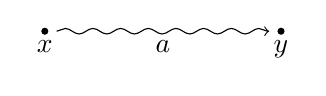
\begin{tikzpicture}[scale=3]
      \draw[decorate, ->, decoration={snake, amplitude=1}]
            (0.05, 0) -- (0.95, 0) node[midway, below]{\(a\)};
      \fill (0, 0) circle[radius=0.015];
      \fill (1, 0) circle[radius=0.015];
      \node[below] () at (0, 0) {\(x\)};
      \node[below] () at (1, 0) {\(y\)};
    \end{tikzpicture}
  \end{center}
  \[
    \Ccell_*(I) \iso \bigg(
    \begin{tikzcd}[row sep=0.1ex]
    	\ZZ\fgen{a} \ar[r] &
        \ZZ\fgen{x, y} \\
    	a \ar[r, mapsto] &
        y - x
    \end{tikzcd}
    \bigg)
  \]
  There is a product cell decomposition for \(I \times I\)
  \begin{center}
  
    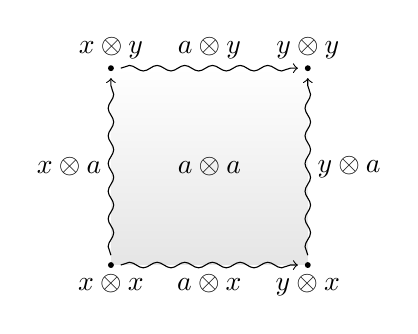
\begin{tikzpicture}[scale=2.5]
      \fill[gray!20, path fading=north] (0, 0) rectangle +(1, 1);
      \draw[decorate, ->, decoration={snake, amplitude=1}]
            (0.05, 0) -- (0.95, 0) node[midway, below]{\(a \otimes x\)};
      \draw[decorate, ->, decoration={snake, amplitude=1}]
            (0.05, 1) -- (0.95, 1) node[midway, above]{\(a \otimes y\)};
      \draw[decorate, ->, decoration={snake, amplitude=1}]
            (0, 0.05) -- (0, 0.95) node[midway, left]{\(x \otimes a\)};
      \draw[decorate, ->, decoration={snake, amplitude=1}]
            (1, 0.05) -- (1, 0.95) node[midway, right]{\(y \otimes a\)};
      \fill (0, 0) circle[radius=0.015];
      \fill (0, 1) circle[radius=0.015];
      \fill (1, 0) circle[radius=0.015];
      \fill (1, 1) circle[radius=0.015];
      \node[below] () at (0, 0) {\(x \otimes x\)};
      \node[below] () at (1, 0) {\(y \otimes x\)};
      \node[above] () at (0, 1) {\(x \otimes y\)};
      \node[above] () at (1, 1) {\(y \otimes y\)};
      \node () at (1/2, 1/2) {\(a \otimes a\)};
    \end{tikzpicture}
  \end{center}
  We can consider some differentials:
  \begin{align*}
    \partial (a \otimes x) &= y \otimes x - x \otimes x \\
      &= (y - x) \otimes x \\
      &= \partial a \otimes x \\
    \partial (a \otimes a)
      &= a \otimes + y \otimes a - a \otimes y - x \otimes a \\
      &= (y - x) \otimes a + a \otimes (x - y) \\
      &= \partial a \otimes a - a \otimes \partial a.
  \end{align*}
\end{example}

\begin{definition}
  Let \(C_*\) and \(D_*\) be two chain complexes of \(R\)-modules.
  Their tensor product \(C_* \otimes_R D_*\) is a chain complex with
  \[
    (C_* \otimes_R D_*) = \bigoplus_{p+q=n} C_p \otimes_R D_q,
  \]
  where the differential is given by
  \[
    \partial(c_p \otimes d_q) = (\partial c_p \otimes d_q) + (-1)^p (c_p \otimes \partial d_q).
  \]
\end{definition}

A good property of this construction is that
\[
  \Ccell_*(X) \otimes \Ccell_*(Y) \iso \Ccell_*(X \times Y).
\]
The homology groups of \(\Ccell_*(X) \otimes \Ccell_*(Y)\) will be computable
purely in terms of \(H_q(X)\) and \(H_q(Y)\).

However, a bad property of this construction is that the homology of
\(C_* \otimes D_*\) is not in general determined by
the homology of \(C_*\) and the homology of \(D_*\).
Moreover, there is no obvious internal \(\Hom\) in chain complexes.








\end{document}

\documentclass{standalone}
\usepackage{chez}

\begin{document}
\chapter{October 19, 2020}

If \(C_*\) and \(D_*\) are chain complexes, then \(\Hom(C_*, D_*)\)
is not obviously a chain complex.


\section{Some algebra}
Suppose
\[
  \begin{tikzcd}
  	0 \ar[r] &
  	A \ar[r] &
  	B \ar[r] &
  	C \ar[r] &
  	0
  \end{tikzcd}
\]
is a short exact sequence of \(R\)-modules and \(M\) is another \(R\)-module.
Then, note that the sequence
\[
  \begin{tikzcd}
  	0 \ar[r] &
  	A \otimes_R M \ar[r] &
  	B \otimes_R M \ar[r] &
  	C \otimes_R M \ar[r] &
  	0
  \end{tikzcd}
\]
is in general not exact.
\begin{example}
  Let \(R = \ZZ\) and consider the short exact sequence
  \[
    \begin{tikzcd}
    	0 \ar[r] &
    	\ZZ \ar[r, "2"] &
    	\ZZ \ar[r] &
    	\ZZ/2\ZZ \ar[r] &
    	0
    \end{tikzcd}
  \]
  Tensoring with \(\ZZ/2\ZZ\) yields
  \[
    \begin{tikzcd}[row sep=0.1ex]
    	0 \ar[r] &
        \ZZ/2\ZZ \otimes_\ZZ \ZZ \ar[r] &
        \ZZ/2\ZZ \otimes_\ZZ \ZZ \ar[r] &
        \ZZ/2\ZZ \otimes_\ZZ \ZZ/2\ZZ \ar[r] &
        0 \\
    	0 \ar[r] &
        \ZZ/2\ZZ \ar[r] &
        \ZZ/2\ZZ \ar[r] &
        \ZZ/2\ZZ \ar[r] &
        0
    \end{tikzcd}
  \]
  However, the multiplication by \(2\) map becomes
  the zero map when we tensor by \(\ZZ/2\ZZ\),
  so the first \(\ZZ/2\ZZ \to \ZZ/2\ZZ\) map becomes \(0\).
  However, the zero map is not injective,
  so the sequence we get is not exact.
\end{example}

\begin{proposition}<module-exactness-tensor>
  If \(M\) is an \(R\)-module, then the functor
  \[
    {-} \otimes_R M \colon \cRmod \to \cRmod
  \]
  is \vocab{right exact}.
  In other words, if
  \[
    \begin{tikzcd}
    	A \ar[r] &
    	B \ar[r] &
    	C \ar[r] &
    	0
    \end{tikzcd}
  \]
  is an exact sequence of \(R\)-modules, then so is
  \[
    \begin{tikzcd}
    	A \otimes_R M \ar[r] &
    	B \otimes_R M \ar[r] &
    	C \otimes_R M \ar[r] &
    	0
    \end{tikzcd}
  \]
\end{proposition}
\begin{corollary}
  In fact,
  \[
    \begin{tikzcd}
    	A \ar[r] &
    	B \ar[r] &
    	C \ar[r] &
    	0
    \end{tikzcd}
  \]
  is exact if and only if
  \[
    \begin{tikzcd}
    	A \otimes_R M \ar[r] &
    	B \otimes_R M \ar[r] &
    	C \otimes_R M \ar[r] &
    	0
    \end{tikzcd}
  \]
  is exact for every \(R\)-module \(M\).
\end{corollary}
\begin{proof*}{Sketch}
  Take \(M = R\).
\end{proof*}

To prove something about tensor products,
it is often helpful to think about
the tensor products as internal \(\Hom\)s.
In particular, we have the related theorem
\begin{proposition}<module-exactness-hom>
  A sequence of \(R\)-modules
  \[
    \begin{tikzcd}
    	A \ar[r] &
    	B \ar[r] &
    	C \ar[r] &
    	0
    \end{tikzcd}
  \]
  is exact if and only if for all \(R\)-modules \(N\),
  \[
    \begin{tikzcd}
    	0 \ar[r] &
    	\ul\Hom_{\cRmod}(C, N) \ar[r] &
    	\ul\Hom_{\cRmod}(B, N) \ar[r] &
    	\ul\Hom_{\cRmod}(A, N)
    \end{tikzcd}
  \]
  is exact.
\end{proposition}

\begin{proof}[\cref{prop:module-exactness-hom} \(\implies\)
  \cref{prop:module-exactness-tensor}]
  Suppose \(A \to B \to C \to 0\) is exact.
  To prove
  \[
    \begin{tikzcd}
    	A \otimes_R M \ar[r] &
    	B \otimes_R M \ar[r] &
    	C \otimes_R M \ar[r] &
    	0
    \end{tikzcd}
  \]
  is exact, by \cref{prop:module-exactness-hom} it suffices to check that
  \[
    \begin{tikzcd}
    	0 \ar[r] &
    	\ul\Hom(C \otimes_R M, N) \ar[r] &
    	\ul\Hom(B \otimes_R M, N) \ar[r] &
    	\ul\Hom(A \otimes_R M, N)
    \end{tikzcd}
  \]
  is exact for every \(N\).
  This is equivalent to checking that
  \[
    \begin{tikzcd}
    	0 \ar[r] &
    	\ul\Hom(C, \ul\Hom(M, N)) \ar[r] &
    	\ul\Hom(B, \ul\Hom(M, N)) \ar[r] &
    	\ul\Hom(A, \ul\Hom(M, N))
    \end{tikzcd}
  \]
  is exact for every \(N\).
  By \cref{prop:module-exactness-hom} again, this is true.
\end{proof}

\begin{proof}[\cref{prop:module-exactness-hom}]
  Suppose
  \(
    \begin{tikzcd}[cramped, column sep=small]
      A \ar[r, "\varphi"] & B \ar[r, "\psi"] & C \ar[r] & 0
    \end{tikzcd}
  \)
  is exact. We want to show
  \[
    \begin{tikzcd}
    	0 \ar[r] &
    	\ul\Hom(C, N) \ar[r] &
    	\ul\Hom(B, N) \ar[r] &
    	\ul\Hom(A, N)
    \end{tikzcd}
  \]
  is exact.

  Exactness at \(\ul\Hom(C, N)\) is equivalent to the map
  \(\ul\Hom(C, N) \to \ul\Hom(B, N)\) being injective.
  This is indeed true, because \(\psi\) is surjective,
  so the composite \(B \to C \to N\) determines a map \(C \to N\).

  Consider the diagram
  \[
    \begin{tikzcd}
    	A \ar[r, "\varphi"] \ar[rd, "0"'] &
        B \ar[r, "\psi"] \ar[d, "f" pos=0.3] &
        C \ar[r] \ar[ld, "g"]&
        0 \\
    	& N & &
    \end{tikzcd}
  \]
  Exactness at \(\ul\Hom(B, N)\) is equivalent to saying that a
  map \(f \colon B \to N\) is restricted to the zero map \(A \to B \to N\)
  if and only if \(f\) can be written as a composite \(B \to C \to N\).
  The backward direction is clear because any composite \(A \to B \to C \to N\)
  is zero because \(A \to B \to C\) is exact.
  We want to find a function \(g \colon C \to N\)
  such that \(f = g \circ \psi\).
  If \(f \circ \varphi = 0\), then note that \(C \iso B / \img \varphi\).
  We can then assign \(g [b] = f b\),
  where \([b]\) denotes the equivalent class representing \(b\).
  This gives \(f = g \circ \psi\), as desired.
\end{proof}

We have now proved that if
\[
  \begin{tikzcd}
  	0 \ar[r] &
  	A \ar[r] &
  	B \ar[r] &
  	C \ar[r] &
  	0
  \end{tikzcd}
\]
is exact and \(M\) is an \(R\)-module, then
\[
  \begin{tikzcd}
  	A \otimes_R M \ar[r] &
  	B \otimes_R M \ar[r] &
  	C \otimes_R M \ar[r] &
  	0
  \end{tikzcd}
\]
is exact, but
\[
  \begin{tikzcd}
  	0 \ar[r] &
  	A \otimes_R M \ar[r] &
  	B \otimes_R M \ar[r] &
  	C \otimes_R M \ar[r] &
  	0
  \end{tikzcd}
\]
is not necessarily exact.

However, if we let \(M = R\), then it is exact.
Furthermore, if we take \(M = R \oplus R\), the sequence will stay exact.
In particular, it will become
\[
  \begin{tikzcd}
    0 \arrow[r] &
    A \oplus A \arrow[r] &
    B \oplus B \arrow[r] &
    C \oplus C \arrow[r] &
    0
  \end{tikzcd}
\]
In general, if \(M\) is a free \(R\)-module, then tensoring with \(M\)
gives an exact sequence and not just a right exact sequence.

\begin{note}
  If \(X\) is a topological space, then \(\Ccell_*(X; R)\) is
  a chain complex of free \(R\)-modules.
\end{note}







\end{document}

\documentclass{standalone}
\usepackage{chez}

\begin{document}
\chapter{October 21, 2020}

\begin{definition}
  Suppose \(C_*\) and \(D_*\) are chain complexes of \(R\)-modules.
  A chain map \(f \colon C_* \to D_*\) is a \vocab{quasi-isomorphism}
  if \(H_q(f)\) is an isomorphism for all \(q\).
  Then, one says that \(C_*\) and \(D_*\) are \vocab{quasi-isomorphic}.
\end{definition}

\begin{definition}
  Suppose \(M\) is an \(R\)-module.
  Then a \vocab{free resolution} of \(M\) is
    a chain complex \(C_*\) of free \(R\)-modules and
    a quasi-isomorphism \(C_* \to M\) where
      we think of \(M\) as a chain complex concentrated in degree \(0\).
\end{definition}

\begin{example}
  Suppose
  \begin{align*}
    C_* &= \Big(
    \begin{tikzcd}[ampersand replacement=\&]
    	\cdots \ar[r] \&
    	0 \ar[r] \&
    	0 \ar[r] \&
    	\ZZ \ar[r, "5"] \&
    	\ZZ \ar[r] \&
    	0 \ar[r] \&
    	\cdots
    \end{tikzcd}
    \Big) \\
    D_* &= \Big(
    \begin{tikzcd}[ampersand replacement=\&]
    	\cdots \ar[r] \&
    	0 \ar[r] \&
    	0 \ar[r] \&
    	0 \ar[r] \&
    	\ZZ/5\ZZ \ar[r] \&
    	0 \ar[r] \&
    	\cdots
    \end{tikzcd}
    \Big)
  \end{align*}
  Then the following chain map is a quasi-isomorphism:
  \[
    \begin{tikzcd}
      \cdots \ar[r] &
        0 \ar[r] \ar[d] &
        \ZZ \ar[r, "5"] \ar[d] &
        \ZZ \ar[r] \ar[d] &
        0 \ar[r] \ar[d] &
        \cdots \\
      \cdots \ar[r] &
        0 \ar[r] &
        0 \ar[r] &
        \ZZ/5\ZZ \ar[r] &
        0 \ar[r] &
        \cdots
    \end{tikzcd}
  \]
  where the map \(\ZZ \to \ZZ/5\ZZ\) is the natural quotient map.
  Moreover, \(C_*\) is a free resolution of \(\ZZ/5\ZZ\).
\end{example}

\begin{example}
  If \(R\) is a field, then every module is its own free resolution.
\end{example}

\begin{example}
  Suppose \(\RR = \ZZ\) and \(M = \ZZ/3\ZZ \oplus \ZZ \oplus \ZZ/2\ZZ\).
  Then we have the free resolution
  \[
    \begin{tikzcd}
    	\cdots \ar[r] &
    		0 \ar[r] \ar[d] &
    		\ZZ \oplus \ZZ \ar[r] \ar[d] &
    		\ZZ \oplus \ZZ \oplus \ZZ \ar[r] \ar[d] &
    		0 \ar[r] \ar[d] &
    		0 \ar[r] \ar[d] &
    		\cdots \\
    	\cdots \ar[r] &
    		0 \ar[r] &
    		0 \ar[r] &
    		\ZZ/3\ZZ \oplus \ZZ \oplus \ZZ/2\ZZ \ar[r] &
    		0 \ar[r] &
    		0 \ar[r] &
    		\cdots
    \end{tikzcd}
  \]
  where the \(\ZZ \oplus \ZZ \to \ZZ \oplus \ZZ \oplus \ZZ\) map
  maps \((1, 0) \mapsto (3, 0, 0)\) and \((0, 1) \mapsto (0, 0, 2)\).
\end{example}

It turns out that we can always find a two term free resolution by
taking a surjection with the degree \(0\) group,
e.g.\ \(\ZZ \oplus \ZZ \oplus \ZZ \to \ZZ/3\ZZ \oplus \ZZ \oplus \ZZ/2\ZZ\)
in the previous example,
and then use the degree \(1\) group to describe the relations.

Note that free resolutions are not unique! In particular,
\[
  \begin{tikzcd}[row sep=0.05ex]
  	\ZZ \ar[r] &
  		\ZZ \oplus \ZZ \oplus \ZZ \ar[r] &
  		\ZZ \oplus \ZZ \oplus \ZZ \\
    1 \ar[r, mapsto] & (0, 0, 1) \\
    & (1, 0, 0) \ar[r, mapsto] & (3, 0, 1) \\
    & (0, 1, 0) \ar[r, mapsto] & (0, 0, 2) \\
    & (0, 0, 1) \ar[r, mapsto] & (0, 0, 0)
  \end{tikzcd}
\]
is also a free resolution of \(\ZZ/3\ZZ \oplus \ZZ \oplus \ZZ/2\ZZ\).
However, it is not ``minimal''.

\begin{example}
  If \(R = \QQ[t]/t^2\) and
    \(M\) is the module \(\QQ\) where \(t\) acts by \(0\),
    then this has a free resolution, but the smallest possible one is infinite.
\end{example}

\begin{theorem}[Fundamental theorem of homological algebra]
  Suppose \(N\) and \(M\) are \(R\)-modules.
  Let
  \[
    \begin{tikzcd}
    	\cdots \ar[r] &
    		F_2 \ar[r] \ar[d] &
    		F_1 \ar[r] \ar[d] &
    		F_0 \ar[d, "\eps_N"] \\
    	\cdots \ar[r] &
    		0 \ar[r] &
    		0 \ar[r] &
    		N
    \end{tikzcd}
    \qquad \text{and} \qquad
    \begin{tikzcd}
    	\cdots \ar[r] &
    		E_2 \ar[r] \ar[d] &
    		E_1 \ar[r] \ar[d] &
    		E_0 \ar[d, "\eps_M"] \\
    	\cdots \ar[r] &
    		0 \ar[r] &
    		0 \ar[r] &
    		M
    \end{tikzcd}
  \]
  be two free resolutions of \(N\) and \(M\) respectively.
  Then any \(R\)-module map \(f \colon N \to M\) lifts to
  a chain map \(f_* \colon F_* \to E_*\).
  Furthermore, \(f_*\) is unique up to chain homotopy.
\end{theorem}

\begin{example}
  Let \(R = \ZZ\), \(N = \ZZ/2\ZZ\), and \(M = \ZZ/6\ZZ\).
  Consider \(f \colon \ZZ/2\ZZ \to \ZZ/6\ZZ\) mapping \(1 \mapsto 3\).
  We have the free resolutions with the maps
  \[
    \begin{tikzcd}[row sep=small,
                   column sep=small,
                   background color=green!6]
    	F_* = \Big( \cdots \ar[rr] &&
    		0 \ar[rr] \ar[ld] &&
    		\ZZ \ar[rr, "2"] \ar[ld, "1"'] &&
    		\ZZ \ar[rr] \ar[ld, "3"'] \ar[dd] &&
    		0 \ar[rr] \ar[ld] &&
    		\cdots \Big) \\
    	E_* = \Big( \cdots \ar[r] &
    		0 \ar[rr] &&
    		\ZZ \ar[rr, "6"'] &&
    		\ZZ \ar[rr, crossing over] \ar[d] &&
    		0 \ar[rr] &&
    		\cdots \Big) \\
    	&& && & \ZZ/6\ZZ & \ZZ/2\ZZ \ar[l, "f"']
    \end{tikzcd}
  \]
  This is a chain map \(f_*\), where
  \[
    \begin{tikzcd}[row sep=tiny]
      \mathllap{H_0(f_*) \colon} H_0(F_*) \ar[r] \ar[d, symbol=\iso] &
        H_0(E_*) \ar[d, symbol=\iso] \\
        \ZZ/2\ZZ \ar[r, "f"] & \ZZ/6\ZZ
    \end{tikzcd}
  \]
\end{example}

This theorem says that if we want to understand maps between modules,
it suffices to understand the maps between their free resolutions
up to chain homotopy.
In particular, they contain the same data,
and the map between the modules can be recovered by taking \(H_0\).

\begin{proof*}{Sketch}
  We can build up a map between the free resolutions inductively,
  checking at every stage that there is only one choice up to chain homotopy.
  To start producing a chain map, if we have
  \[
    \begin{tikzcd}
      F_0 \arrow[d, dashed, "f_0"] \arrow[r, "\eps_N"] &
        N \arrow[d, "f"] \\
      E_0 \arrow[r, "\eps_M"] &
        M
    \end{tikzcd}
  \]
  we want to produce the dashed \(f_0\) map.
  Since \(F_0\) is free, say on \(S_0\), for each \(s_0 \in S_0\),
  we can define \(f_0(s_0)\) to be any element in \(E_0\) such that
  \[
    \eps_M(f_0 s_0) = f (\eps_N s_0).
  \]
  This is possible because \(\eps_M\) is surjective,
  because \(M\) is the homology of \(E_*\),
  which means \(M\) is the quotient of
  \(E_0\) mod the image of the \(E_1 \to E_0\) map.
  
  This gives the diagram
  \[
    \begin{tikzcd}
      \ker \eps_M \arrow[d, "g_0"] \arrow[r] &
      F_0 \arrow[d, "f_0"] \arrow[r, "\eps_N"] &
        N \arrow[d, "f"] \\
      \ker \eps_N \arrow[r] &
      E_0 \arrow[r, "\eps_M"'] &
        M
    \end{tikzcd}
  \]
  where the map \(g_0\) is unique because \(\ker \eps_M \to F_0\)
  and \(\ker \eps_N \to E_0\) are just projections,
  so \(f_0\) determines \(g_0\).

  Now we wish to produce the dashed map in the diagram
  \[
    \begin{tikzcd}
      F_1 \ar[r] \ar[d, dashed, "f_1"] &
      \ker \eps_M \arrow[d, "g_0"] \arrow[r] &
      F_0 \arrow[d, "f_0"] \arrow[r, "\eps_N"] &
        N \arrow[d, "f"] \\
      E_1 \ar[r] &
      \ker \eps_N \arrow[r] &
      E_0 \arrow[r, "\eps_M"'] &
        M
    \end{tikzcd}
  \]
  However, by exactness of the free resolutions,
  we know that the \(F_1 \to \ker \eps_N\) and \(E_1 \to \ker \eps_M\) maps
  are surjective, so we can apply the same argument as before.
\end{proof*}

\begin{adhoctheorem}{Definition Sketch}
  Let \(R\) be a commutative ring, and \(\cchRmod\) be the category
  of chain complexes of \(R\)-modules.
  The \vocab{derived category} of \(R\), denoted \(\der(R)\),
  is the category obtained from \(\cchRmod\) by formally inverting
  all quasi-isomorphisms.

  In other words, the objects of \(\der(R)\) are the objects of \(\cchRmod\),
  but there are many more morphisms than just chain maps.
  In particular, if \(f_* \colon C_* \to D_*\) is a chain map,
  then there is a formal inverse \(g \colon D_* \to C_*\) in \(\der(R)\).
\end{adhoctheorem}
The formal construction of \(\der(R)\) is beyond the scope of the class
because there are set-theoretic technicalities.

In algebraic topology, we don't actually care about \(\cchRmod\).
We only care about \(\der(R)\).

\begin{example}
  In \(\der(R)\), every object is isomorphic to
  a chain complex of free modules.
  Free resolutions are an example of this.
\end{example}

We will state facts about \(\der(R)\) and then
prove consequences of these facts that can be stated
without reference to \(\der(R)\).
The reason we do so is because it gives motivation for the statements
and their proofs.

\begin{example}[Tensor products in \(\der(R)\)]
  If \(C_*\) and \(D_*\) are two chain complexes,
  we define the \vocab{derived tensor product}
  \(C_* \otimes^{\mathbb L} D_*\) as follows:
  \begin{enumerate}[nosep]
    \item We replace \(C_*\) and \(D_*\) by quasi-isomorphic chain complexes
          of free modules \(C_*'\) and \(D_*'\).
    \item Take \(C_*' \otimes_R D_*'\).
    \item The result is well defined up to quasi-isomorphism
  \end{enumerate}
\end{example}










\end{document}

\documentclass{standalone}
\usepackage{chez}

\begin{document}
\chapter{October 23, 2020}

If two chain complexes are isomorphic in \(\der(R)\),
then they have isomorphic homology \(R\)-modules.

\begin{fact}
  If at least one of \(C_*\) and \(D_*\) are
  chain complexes of free \(R\)-modules,
  then \(C_* \otimes_R^{\mathbb L} D_* \iso C_* \otimes_R D_*\).
\end{fact}
Since we haven't described the derived category rigorously,
we can't prove this. However, we will show some consequences of this fact.

\begin{definition}
  If \(M\) and \(N\) are two \(R\)-modules,
  then the \vocab{\(\Tor\)} functor is defined to be
  \(\Tor_i(M, N) \coloneqq H_i(M \otimes^{\mathbb L}_R N)\),
  where \(M\) and \(N\) are viewed as
  chain complexes concentrated in degree \(0\).
\end{definition}
Soon we will prove that \(\Tor_i(M, N)\) are well defined.
For now, let's do some calculations of them.

\begin{example}
  Suppose \(R = \ZZ\). Then we can compute
  \(\ZZ/2\ZZ \otimes^{\mathbb L}_\ZZ \ZZ/4\ZZ\)
  by replacing either \(\ZZ/2\ZZ\) or \(\ZZ/4\ZZ\) with their free resolution,
  and then take the tensor product normally.

  We can compute this by resolving \(\ZZ/2\ZZ\), i.e.\ replacing it with
  its free resolution.
  \begin{align*}
    \ZZ/2\ZZ \otimes^{\mathbb L} \ZZ/4\ZZ
      &\iso \Big(
        \begin{tikzcd}[ampersand replacement=\&,
                       cramped, column sep=scriptsize]
          \ZZ \ar[r, "2"] \& \ZZ
        \end{tikzcd}
      \Big) \otimes \ZZ/4\ZZ \\
      &\iso \Bigg(\;
        \begin{tikzcd}[ampersand replacement=\&,
                       cramped, column sep=scriptsize, row sep=0ex]
          \cdots \ar[r] \&
          0 \ar[r] \&
          \ZZ/4\ZZ \ar[r, "2"] \&
          \ZZ/4\ZZ \ar[r] \&
          0 \ar[r] \&
          \cdots \\
          \& \& \deg 1 \& \deg 0
        \end{tikzcd}
      \;\Bigg)
  \end{align*}
  Then we have
  \begin{align*}
    \Tor_0(\ZZ/2\ZZ, \ZZ/4\ZZ) &= \frac{\ZZ/4\ZZ}{\ZZ/2\ZZ} \iso \ZZ/2\ZZ \\
    \Tor_1(\ZZ/2\ZZ, \ZZ/4\ZZ) &= \frac{\ZZ/2\ZZ}{0} \iso \ZZ/2\ZZ,
  \end{align*}
  and \(\Tor_i = 0\) for all other \(i\).

  We can also compute it by resolving \(\ZZ/4\ZZ\):
  \begin{align*}
    \ZZ/2\ZZ \otimes^{\mathbb L} \ZZ/4\ZZ
      &\iso \ZZ/2\ZZ \otimes \Big(
        \begin{tikzcd}[ampersand replacement=\&,
                       cramped, column sep=scriptsize]
          \ZZ \ar[r, "4"] \& \ZZ
        \end{tikzcd}
      \Big) \\
      &\iso \Big(
        \begin{tikzcd}[ampersand replacement=\&,
                       cramped, column sep=scriptsize]
          \ZZ/4\ZZ \ar[r, "4"] \& \ZZ/4\ZZ
        \end{tikzcd}
      \Big)
  \end{align*}
  Then we have
  \begin{align*}
    \Tor_0(\ZZ/2\ZZ, \ZZ/4\ZZ) &= \frac{\ZZ/2\ZZ}{0} \iso \ZZ/2\ZZ \\
    \Tor_1(\ZZ/2\ZZ, \ZZ/4\ZZ) &= \frac{\ZZ/2\ZZ}{0} \iso \ZZ/2\ZZ,
  \end{align*}
  and \(\Tor_i = 0\) for all other \(i\).

  We can also compute this in some more inefficient ways.
  We can resolve both sides:
  \begin{align*}
    \ZZ/2\ZZ \otimes^{\mathbb L} \ZZ/4\ZZ
      &\iso \Big(
        \begin{tikzcd}[ampersand replacement=\&,
                       cramped, column sep=scriptsize]
          \ZZ\fgen{a} \ar[r, "2"] \& \ZZ\fgen{b}
        \end{tikzcd}
      \Big) \otimes \Big(
        \begin{tikzcd}[ampersand replacement=\&,
                       cramped, column sep=scriptsize]
          \ZZ\fgen{c} \ar[r, "4"] \& \ZZ\fgen{d}
        \end{tikzcd}
      \Big),
  \intertext{where we add generators to make it more clear. Multiplying,}
    &\iso \begin{tikzcd}[ampersand replacement=\&,
                         cramped, column sep=scriptsize]
      \ZZ\fgen{a \otimes c} \ar[r, "\partial_2"] \&
        \ZZ\fgen{b \otimes c, a \otimes d} \ar[r, "\partial_1"] \&
        \ZZ\fgen{b \otimes d}
    \end{tikzcd}
  \end{align*}
  where
  \begin{align*}
    \partial(a \otimes c) &=        (\partial a \otimes c)
                             + (-1) (a \otimes \partial c)
                           = (2b \otimes c) - (a \otimes 4d) \\
    \partial(b \otimes c) &=   (\partial b \otimes c)
                             + (b \otimes \partial c)
                           = 4 (b \otimes d) \\
    \partial(a \otimes d) &=        (\partial a \otimes d)
                             + (-1) (a \otimes \partial d)
                           = 2 (b \otimes d).
  \end{align*}
  We can also confirm
  \[
    \partial \partial (a \otimes c)
      = \partial (2(b \otimes c) - 4(a \otimes d))
      = 2 \cdot 4(b \otimes d) - 4 \cdot 2(b \otimes d)
      = 0.
  \]
  We can then compute \(H_0\) of this complex to be
  \(\frac{\ZZ\fgen{b \otimes d}}{\img \partial_1} = \ZZ/2\ZZ\),
  and \(H_1\) to be
  \(
    \ker \partial_1 / \img \partial_2
      = \frac{\ZZ\fgen{ b \otimes c - 2(a \otimes d)}}
             {\ZZ\fgen{2b \otimes c - 4(a \otimes d)}}
      \iso \ZZ/2\ZZ
  \).
  Moreover, we can notice \(\partial_2\) is injective,
  so all higher order homology groups are zero, as expected.
\end{example}

\begin{example}
  To compute \(\Tor_i(\ZZ/2\ZZ, \ZZ/3\ZZ)\), we have
  \begin{align*}
    \ZZ/2\ZZ \otimes^{\mathbb L} \ZZ/3\ZZ
      &\iso \Big(
        \begin{tikzcd}[ampersand replacement=\&,
                       cramped, column sep=scriptsize]
          \ZZ \ar[r, "2"] \& \ZZ
        \end{tikzcd}
      \Big) \otimes \ZZ/3\ZZ \\
      &\iso \begin{tikzcd}[ampersand replacement=\&,
                           cramped, column sep=scriptsize]
          \ZZ/3\ZZ \ar[r, "2"] \& \ZZ/3\ZZ
        \end{tikzcd}
  \end{align*}
  which means
  \begin{align*}
    \Tor_0(\ZZ/2\ZZ, \ZZ/3\ZZ) &\iso 0 \\
    \Tor_1(\ZZ/2\ZZ, \ZZ/3\ZZ) &\iso 0.
  \end{align*}
\end{example}

\begin{example}
  For \(\Tor_i(\ZZ/3\ZZ, \ZZ)\), note that
  \[
    \ZZ/3\ZZ \otimes^{\mathbb L} \ZZ \iso \ZZ/3\ZZ,
  \]
  where we interpret \(\ZZ/3\ZZ\) as
  \[
    \begin{tikzcd}
      \cdots \ar[r] &
        0 \ar[r] &
        \ZZ/3\ZZ \ar[r] &
        0 \ar[r] &
        \cdots
    \end{tikzcd}
  \]
  so
  \[
    \Tor_0(\ZZ/3\ZZ, \ZZ) \iso \ZZ/3\ZZ
  \]
  and \(\Tor_i = 0\) for all other \(i\).
\end{example}

\begin{example}
  If \(R\) is a field, and \(V\) and \(W\) are vector spaces over \(R\),
  then \(\Tor_0(V, W) \iso V \otimes_R W\) and \(\Tor_i(V, W) \iso 0\)
  for all other \(i\).
\end{example}

We will now prove that the \(\Tor\) groups are well defined
without reference to the derived categories.
\begin{proof}[\(\Tor\) groups are well defined]
  Suppose \(M\) and \(N\) are two \(R\)-modules, and suppose
  \(F_*\) and \(F_*'\) are two free resolutions of \(M\).
  We will prove that \(F_* \otimes_R N\) and \(F_*' \otimes_R N\)
  have the same homology groups.
  In fact, we will show that they are chain homotopy equivalent.

  By the fundamental theorem of homological algebra,
  there exists a unique (up to chain homotopy) map
  \(f \colon F_* \to F_*'\) lifting \(1_M\) and
  \(g \colon F_*' \to F_*\) lifting \(1_M\).

  Note that \(f \circ g\) is a map from \(F_*' \to F_*'\) lifting \(1_M\),
  so by the fundamental theorem,
  \(f \circ g\) must be chain homotopic to \(1_{F_*'}\).
  It follows that
  \((f \circ g) \otimes_R N = (f \otimes N) \circ (g \otimes N)\),
  which is chain homotopic to \(1_{F_*' \otimes N}\).

  Similarly, \((g \circ f) \otimes_R N\) is chain homotopic to
  \(1_{F_* \otimes N}\).
  Therefore, \(g \otimes_R N\) and \(f \otimes_R N\) are inverses
  up to chain homotopy.
  This proves that \(F_* \otimes_R N\) and \(F_*' \otimes_R N\)
  are chain homotopy equivalent.
\end{proof}

\subsection{On internal \texorpdfstring{\(\Hom\)}{Hom}s}
\begin{definition}
  If \(F_*\) is a chain complex of free \(R\)-modules and
  \(N\) is an \(R\)-module, considered as a chain concentrated in degree \(0\).
  Then we may form a new chain complex \(\ul\Hom_{\der(R)}(F_*, N)\)
  with
  \[
    \ul\Hom(F_*, N)_n = \ul\Hom_{\cRmod}(F_{-n}, N).
  \]
\end{definition}

\begin{example}
  If \(R = \ZZ\),
  \[
    F_* = \bigg(\begin{tikzcd}[row sep=-1ex]
      \cdots \ar[r] &
        0 \ar[r] &
        \ZZ \ar[r, "4"] &
        \ZZ \ar[r] &
        0 \ar[r] &
        \cdots \\
      & & \deg 1 & \deg 0
    \end{tikzcd}
    \bigg)
  \]
  and \(N = \ZZ/2\ZZ\).
  Then
  \[
    \ul\Hom_{\der(\ZZ)}(F_*, N) \iso
    \bigg(
      \begin{tikzcd}[row sep=-1ex]
        \cdots \ar[r] &
          0 \ar[r] &
          \ZZ/2\ZZ \ar[r, "\partial"] &
          \ZZ/2\ZZ \ar[r] &
          0 \ar[r] &
          \cdots \\
        & & \deg 0 & \deg {-1}
      \end{tikzcd}
    \bigg)
  \]
  The degree \(0\) \(R\)-module is
  \(\ul\Hom(F_0, N) \iso \ul\Hom(\ZZ, \ZZ/2\ZZ) \iso \ZZ/2\ZZ\),
  and the degree \(1\) \(R\)-module is \(\ul\Hom(F_1, N) \iso \ZZ/2\ZZ\).

  We can see that the differential \(\partial\) exists because
  given a map in \(\ul\Hom(F_0, N)\),
  we can compose it with the \(4\) map to get a map in \(\ul\Hom(F_1, N)\).
\end{example}

\begin{definition}
  If \(M\) and \(N\) are \(R\)-modules, then \(\ul\Hom_{\der(R)}(M, N)\)
  can be computed by replacing \(M\) with a free resolution and
  then applying the above construction.
\end{definition}

\begin{definition}
  If \(M\) and \(N\) are \(R\)-modules, then the \vocab{\(\Ext\) functor} is
  \begin{align*}
    \Ext_R^i(M, N) &= H_{-i}(\ul\Hom_{\der(R)}(M, N)) \\
      &= H_{-i}(\ul\Hom_{\der(R)}(F_*, N)),
  \end{align*}
  where \(F_*\) is any free resolution of \(M\).
\end{definition}

We will use \(\Tor\) and \(\Ext\) to compute homology with coefficients from
homology with \(\ZZ\) coefficients.






\end{document}

\documentclass{standalone}
\usepackage{chez}

\begin{document}
\chapter{October 26, 2020}

\subsection{Homology with coefficients}
Recall that if \(X\) is a topological space,
we have chain complex of \(R\)-modules \(S_*(X; R)\) with
the \(n\)th group being the free \(R\)-module generated by \(\Sing_n(X)\).
The \(\partial\) maps are given by the alternating sums of the \(d_i\) maps.

\begin{note}
  \(S_*(X; R)\) may be alternatively described as \(S_*(X) \otimes_\ZZ R\),
  which also calculates the derived tensor product.
\end{note}

We can even make a more general definition
\begin{definition}
  Suppose \(M\) is an abelian group and \(X\) is a topological space.
  We can define \(S_*(X; M) \coloneqq S_*(X) \otimes_\ZZ M\)
  and \(H_q(X; M)\) to be \(H_q\) of \(S_*(X; M)\).
\end{definition}

If \(R\) is a commutative ring and \(M\) is an \(R\)-module,
then \(H_q(X; M)\) acquires the structure of an \(R\)-module.

\subsection{Cohomology}
Suppose \(X\) is a topological space and \(M\) is an abelian group.
We can make a chain complex, concentrated in non-positive degrees,
with the \((-n)\)th term
\(
  \ul\Hom_{\cat{\ZZ\text{-}mod}}(S_n(X), M) % chktex 35
\).
This new chain complex calculates \(\ul\Hom_{\der(\ZZ)}(S_*(X), M)\).

\begin{definition}
  The \((-q)\)th homology group of the above chain complex is denoted
  \(H^q(X; M)\), and is called the \(q\)th \vocab{cohomology group}
  of \(X\) with coefficients in \(M\).
\end{definition}

Both homology coefficients and cohomology with coefficients can
be determined by homology with integer coefficients.
However, these may be easier to compute, so they can be useful.

\subsection{Universal coefficient theorems}
\begin{theorem}[For cohomology]
  Let \(X\) be a topological space, and \(M\) be an abelian group.
  For any integer \(q\), there is an isomorphism
  \[
    H^q(X; M) \iso \ul\Hom_\cAb(H_q(X), M) \oplus \Ext^1_\ZZ(H_{q-1}(X), M).
  \]
\end{theorem}
Note that on the right side, we have expressions that only deal
with homology with integer coefficients, and on the left
we have homology with coefficients in an arbitrary abelian group \(M\).

\begin{theorem}[For homology]<homology-universal-coefficient>
  Let \(C_*\) be a chain complex of free \(\ZZ\)-modules
  (e.g.\ \(C_* = S_*(X)\) or \(C_* = \Ccell_*(X)\))
  and \(M\) is an abelian group.
  Then there is a natural short exact sequence
  \[
    \begin{tikzcd}
      0 \arrow[r] &
      H_q(C_*) \otimes_\ZZ M \arrow[r] &
      H_q(C_* \otimes_\ZZ M) \arrow[r] &
      \Tor_1(H_{q-1}(C_*), M) \arrow[r] &
      0
    \end{tikzcd}
  \]
  and furthermore an isomorphism
  \[
    H_q(C_* \otimes_\ZZ M)
      \iso H_q(C_*) \otimes_\ZZ M \oplus \Tor_1^{\ZZ}(H_{q-1}(C_*), M).
  \]
\end{theorem}
Note that similarly to the previous theorem,
the left is calculating homology with coefficients
but the right side is about homology with integer coefficients.

\begin{adhoctheorem}{Warning}<warning:unnatural-isomorphism>
  This isomorphism in \cref{thm:homology-universal-coefficient} is not natural!
  While the short exact sequence is natural,
  the direct sum decomposition of the middle term is not natural.
\end{adhoctheorem}

Let's do some computations before we prove this.
\begin{example}
  Consider \(\RP^2\).
  Recall that
  \[
    \Ccell_*(\RP^2) = \Ccell_*(\RP^2; \ZZ) \iso \begin{tikzcd}
        \ZZ \ar[r, "2"] & \ZZ \ar[r, "0"] & \ZZ
    \end{tikzcd}
  \]
  and we have
  \[
    H_q(\RP^2) = \begin{cases*}
      \ZZ & \(q = 0\) \\[-1ex]
      \ZZ/2\ZZ{} & \(q = 1\) \\[-1ex]
      0 & otherwise.
    \end{cases*}
  \]
  We can then as what \(H_q(\RP^2; \FF_2)\) are.

  One way we can compute this is to calculate
  \(\Ccell_*(\RP^2) \otimes_\ZZ \FF_2\) directly.
  \[
    \begin{tikzcd}
      \FF_2 \ar[r, "2"] & \FF_2 \ar[r, "0"] & \FF_2
    \end{tikzcd}
  \]
  This gives
  \[
    H_q(\RP^2; \FF_2) = \begin{cases*}
      \FF_2 & \(q = 0, 1, 2\) \\[-1ex]
      0 & otherwise.
    \end{cases*}
  \]
  
  The other way we can compute this is to use
  the universal coefficients theorem.
  In particular, we have
  \begin{align*}
    H_2(\RP^2; \FF_2) &\iso H_2(\RP^2) \otimes_\ZZ \FF_2
                          \oplus_\ZZ \Tor_1(H_1(\RP^2), \FF_2) \\
      &\iso 0 \otimes_\ZZ F_2 \oplus \Tor_1(\FF_2, \FF_2) \\
      &\iso 0 \oplus H_1(\FF_2 \otimes^{\mathbb L}_\ZZ \FF_2).
  \end{align*}
  We know
  \begin{align*}
    H_1(\FF_2 \otimes^{\mathbb L}_\ZZ \FF_2)
      &= H_1\parens[\Big]{
        \parens[\Big]{\begin{tikzcd}[ampersand replacement=\&]
          \ZZ \ar[r, "2"] \& \ZZ
        \end{tikzcd}}
        \otimes_\ZZ \FF_2
      } \\
      &= H_1\parens[\Big]{
        \begin{tikzcd}[ampersand replacement=\&]
          \FF_2 \ar[r, "2"] \& \FF_2
        \end{tikzcd}} \\
      &= \FF_2,
  \end{align*}
  so \(H_2(\RP^2; \FF_2) = \FF_2\), as expected.

  Similarly, we have
  \begin{align*}
    H_1(\RP^2; \FF_2) &\iso H_1(\RP^2) \otimes_\ZZ \FF_2
                          \oplus_\ZZ \Tor_1(H_0(\RP^2), \FF_2) \\
      &\iso \FF_2 \otimes_\ZZ F_2 \oplus \Tor_1(\ZZ, \FF_2) \\
      &\iso \FF_2 \oplus H_1(\ZZ \otimes^{\mathbb L} \FF_2) \\
      &\iso \FF_2 \oplus H_1\parens[\Big]{
        \begin{tikzcd}[ampersand replacement=\&, column sep=scriptsize]
          \cdots \ar[r] \& 0 \ar[r] \& \FF_2 \ar[r] \& 0 \ar[r] \& \cdots
        \end{tikzcd}
      } \\
      &\iso \FF_2 \oplus 0 = \FF_2,
  \end{align*}
  as desired.
\end{example}

\begin{example}
  Let's compute \(H_2(S^2; \FF_3)\). We have
  \begin{align*}
    H_2(S^2; \FF_3) &\iso H_2(S^2) \otimes_\ZZ \FF_3
                          \oplus_\ZZ \Tor_1(H_1(S^2), \FF_3) \\
      &\iso \ZZ \otimes_\ZZ F_3 \oplus \Tor_1(0, \FF_3) \\
      &\iso \FF_3 \oplus H_1(0 \otimes^{\mathbb L} \FF_2) \\
      &\iso \FF_2 \oplus H_1\parens[\big]{
        \begin{tikzcd}[ampersand replacement=\&, column sep=scriptsize]
          \cdots \ar[r] \& 0 \ar[r] \& 0 \ar[r] \& \cdots
        \end{tikzcd}
      } \\
      &\iso \FF_3 \oplus 0 = \FF_3,
  \end{align*}
\end{example}

\begin{proof}[\cref{thm:homology-universal-coefficient}]
  Suppose \(C_*\) is a chain complex of free \(\ZZ\)-modules and
          \(M\) is an abelian group.
  We want to calculate the homology groups of \(C_* \otimes_\ZZ M\).
  Consider a free resolution
  \[
    \begin{tikzcd}
      \cdots \ar[r] &
        0 \ar[r] &
        F_1 \ar[r] &
        F_0 \ar[r] &
        0 \ar[r] &
        \cdots
    \end{tikzcd}
  \]
  of \(M\).
  Since \(\ZZ\) is a PID, we can find this two-term free resolution.
  This gives us a short exact sequence of chain complexes
  \[
    \begin{tikzcd}
      0 \arrow[r] &
      C_* \otimes_\ZZ F_1 \arrow[r] &
      C_* \otimes_\ZZ F_0 \arrow[r] &
      C_* \otimes_\ZZ M \arrow[r] &
      0
    \end{tikzcd}
  \]
  which gives us a long exact sequence in homology
  \[
    \begin{tikzcd}[row sep=scriptsize]
      \cdots \ar[r] &
        H_q    (C_* \otimes F_1) \ar[d, symbol=\iso] \ar[r] &
        H_q    (C_* \otimes F_0) \ar[d, symbol=\iso] \ar[r] &
        H_q    (C_* \otimes M  ) \ar[d, symbol=\iso] \ar[r, "\partial"] &
        H_{q-1}(C_* \otimes F_1) \ar[d, symbol=\iso] \ar[r] &
        H_{q-1}(C_* \otimes F_0) \ar[d, symbol=\iso] \ar[r] &
        \cdots \\
      \cdots \ar[r] &
        H_q    (C_*) \otimes F_1 \ar[r] &
        H_q    (C_*) \otimes F_0 \ar[r] &
        H_q    (C_* \otimes M)   \ar[r] &
        H_{q-1}(C_*) \otimes F_1 \ar[r] &
        H_{q-1}(C_*) \otimes F_0 \ar[r] &
        \cdots
    \end{tikzcd}
  \]
  This long exact sequence implies the short exact sequence
  \[
    \begin{tikzcd}
      0 \arrow[r] &
        H_q(C_*) \otimes F_0/F_1 \arrow[r] &
        H_q(C_* \otimes M) \arrow[r] &
        \ker\brackets{
          H_{q-1}(C_*) \otimes F_1 \to H_{q-1}(C_*) \otimes F_0
        } \arrow[r] &
        0
    \end{tikzcd}
  \]
  Since \(F_1 \to F_0 \to M\) is a free resolution, we have
  \(F_0/F_1 \iso M\).
  Also, the third term of the short exact sequence is
  \(\Tor(H_{q-1}(C_*), M)\).
  This gives the short exact sequence
  \[
    \begin{tikzcd}
      0 \arrow[r] &
        H_q(C_*) \otimes M \arrow[r] &
        H_q(C_* \otimes M) \arrow[r] &
        \Tor_1(H_{q-1}(C_*), M) \arrow[r] &
        0
    \end{tikzcd}\pog
  \]
\end{proof}











\end{document}

\documentclass{standalone}
\usepackage{chez}

\begin{document}
\chapter{October 28, 2020}

\begin{question}
  What is the homology of a tensor product of chain complexes?
\end{question}

\begin{theorem}
  Suppose that \(C_*\) and \(D_*\) are chain complexes of \(\ZZ\)-modules
  and suppose \(C_*\) is a complex of free \(\ZZ\)-modules. Then
  \[
    H_n(C_* \otimes_\ZZ D_*)
      = \parens*{\bigoplus_{p + q = n} H_p(C_*) \otimes_\ZZ H_q(D_*)} \oplus
        \parens*{\bigoplus_{p + q = n-1} \Tor_1^{\ZZ}(H_p(C_*), H_q(D_*))}.
  \]
\end{theorem}

Note the similarity between this theorem and the universal coefficient theorem.
We have a guess for the tensor product in the first term,
and then correction terms described by the \(\Tor\) functor.
In fact, the universal coefficient theorem is a special case of this theorem,
where \(D_*\) is concentrated in degree \(0\).

\begin{proof*}{Proof idea 1}
  Note that \(C_* \otimes D_*\) calculates
  \(C_* \otimes^{\mathbb L} D_*\) in \(\der(\ZZ)\).
  Its homology will not change if we replace \(D_*\) with
  any chain complex isomorphic to \(D_*\) in \(\der(\ZZ)\).
  In particular, replace \(D_*\) with the chain complex \(D_*'\)
  such that \((D_*')_q = H_q(D_*)\) and all of the maps are \(0\) maps.
  Note that \(D_*'\) is a direct sum of
  chain complexes concentrated in single degrees,
  so we can reduce the theorem to the universal coefficient theorem.
\end{proof*}

However, we may want to give a proof that does not use
the derived category, since we have not talked about those rigorously.
This proof will still however, have the same spirit, since we will
reduce the proof to the universal coefficient theorem.
\begin{proof*}{Proof idea 2}
  Consider the new chain complex \(Z(D_*)\) where
  \[
    Z(D_*)_n = Z_n(D_*) = \ker(\partial \colon D_n \to D_{n-1})
  \]
  and all \(\partial\) maps in \(Z(D_*)\) are \(0\).
  Note that the is an inclusion of chain complexes \(Z(D_*) \to D_*\).
  \(Z(D_*)\) is a direct sum of chain complexes concentrated in single degrees.
  
  Note that the quotient chain complex \(D_*/Z(D_*)\) also has boundary maps
  that are the zero maps.
  Therefore, \(D_* / Z(D_*)\) is also a direct sum of chain complexes
  concentrated in single degrees.

  Consider the short exact sequence of chain complexes
  \[
    \begin{tikzcd}
      0 \arrow[r] &
      C_* \otimes_\ZZ Z(D_*) \arrow[r] &
      C_* \otimes_\ZZ D_* \arrow[r] &
      C_* \otimes_\ZZ D_*/Z(D_*) \arrow[r] &
      0
    \end{tikzcd}
  \]
  This gives the long exact sequence in homology from the snake lemma
  to write \(H_n(C_* \otimes_\ZZ D_*)\) in terms of
  \(H_n(C_* \otimes_\ZZ Z(D_*))\) and \(H_{n-1}(C_* \otimes_\ZZ D_*/Z(D_*))\).
  This reduces to the universal coefficient theorem.
\end{proof*}

\begin{remark}
  This extends to all PIDs, not just \(\ZZ\).
  Suppose that \(R\) is a PID and
  \(C_*\) and \(D_*\) are chain complexes of \(R\)-modules
  such that \(C_*\) is a chain complex of free \(R\)-modules.
  Then
  \[
    H_n(C_* \otimes_R D_*) \iso
      \parens*{\bigoplus_{p + q = n} H_p(C_*) \otimes_R H_q(D_*)} \oplus
      \parens*{\bigoplus_{p + q = n-1} \Tor_1^R(H_p(C_*), H_q(D_*))}.
  \]
\end{remark}
The hypothesis that \(R\) has to be a PID comes from how we needed a
\(2\)-term free resolution of \(M\) in the proof of
the universal coefficient theorem.

In particular, if \(R\) is a field, then
\[
  H_n(C_* \otimes_R D_*) \iso \bigoplus_{p+q = n} H_p(C_*) \otimes_R H_q(D_*).
\]
This is because all free resolutions over a field are not interesting,
so all of the \(\Tor\) functors vanish.

\begin{theorem}[Eilenberg-Zilber]<eilenberg-zilber>
  Suppose \(X\) and \(Y\) are topological spaces
  and \(R\) is a commutative ring.
  Then \(S_*(X \times Y; R)\) is quasi-isomorphic to
  \(S_*(X; R) \otimes_R S_*(Y; R)\).
\end{theorem}
\begin{proof*}{Proof idea 1}
  If \(X\) and \(Y\) are CW complexes,
  then we can examine the CW structure on \(X \times Y\).
  Rather than developing the theory of product CW structures,
  we will directly prove the theorem instead,
  since not all topological spaces have a natural CW structure.
\end{proof*}

Before we prove the theorem, let's do some examples.
\begin{example}
  Let's compute the groups \(H_q(\RP^2 \times \RP^2; \FF_2)\).
  Recall that we have
  \[
    H_q(\RP^2; \FF_2) = \begin{cases*}
      \FF_2 & \(q = 0, 1, 2\) \\[-1ex]
      0 & otherwise.
    \end{cases*}
  \]
  Since \(\FF_2\) is a field, this means
  \begin{align*}
    H_0(\RP^2 \times \RP^2; \FF_2)
      &\iso \bigoplus_{p + q = 0} H_p(\RP^2; \FF_2) \otimes_{\FF_2}
                                  H_q(\RP^2; \FF_2) \\
      &\iso H_0(\RP^2; \FF_2) \otimes_{\FF_2} H_0(\RP^2; \FF_2) \\
      &\iso \FF_2 \otimes_{\FF_2} \FF_2 \\
      &\iso \FF_2 \\
    %
    H_1(\RP^2 \times \RP^2; \FF_2)
      &\iso \bigoplus_{p + q = 1} H_p(\RP^2; \FF_2) \otimes_{\FF_2}
                                  H_q(\RP^2; \FF_2) \\
      &\iso H_0(\RP^2; \FF_2) \otimes_{\FF_2} H_1(\RP^2; \FF_2) \oplus
            H_1(\RP^2; \FF_2) \otimes_{\FF_2} H_0(\RP^2; \FF_2) \\
      &\iso \FF_2 \otimes_{\FF_2} \FF_2 \oplus \FF_2 \otimes_{\FF_2} \FF_2 \\
    %
    H_2(\RP^2 \times \RP^2; \FF_2)
      &\iso (H_0 \otimes H_2) \oplus
            (H_1 \otimes H_1) \oplus
            (H_2 \otimes H_0) \\
      &\iso \FF_2 \oplus \FF_2 \oplus \FF_2 \\
    %
    H_3(\RP^2 \times \RP^2; \FF_2)
      &\iso (H_0 \otimes H_3) \oplus
            (H_1 \otimes H_2) \oplus
            (H_2 \otimes H_1) \oplus
            (H_3 \otimes H_0) \\
      &\iso (\FF_2 \otimes 0    ) \oplus
            (\FF_2 \otimes \FF_2) \oplus
            (\FF_2 \otimes \FF_2) \oplus
            (0     \otimes \FF_2) \\
      &\iso \FF_2 \oplus \FF_2 \\
    %
    H_4(\RP^2 \times \RP^2; \FF_4)
      &\iso (H_0 \otimes H_4) \oplus
            (H_1 \otimes H_3) \oplus
            (H_2 \otimes H_2) \oplus
            (H_3 \otimes H_1) \oplus
            (H_4 \otimes H_0) \\
      &\iso (\FF_2 \otimes 0    ) \oplus
            (\FF_2 \otimes 0    ) \oplus
            (\FF_2 \otimes \FF_2) \oplus
            (0     \otimes \FF_2) \oplus
            (0     \otimes \FF_2) \\
      &\iso \FF_2.
  \end{align*}
  This gives
  \[
    H_q(\RP^2 \times \RP^2; \FF_2) \iso \begin{cases}
      \FF_2                           & q = 0            \\[-1ex]
      \FF_2 \oplus \FF_2              & q = 1            \\[-1ex]
      \FF_2 \oplus \FF_2 \oplus \FF_2 & q = 2            \\[-1ex]
      \FF_2 \oplus \FF_2              & q = 3            \\[-1ex]
      \FF_2                           & q = 4            \\[-1ex]
      0                               & \text{otherwise.}
    \end{cases}
  \]
  One thing to note is that these groups are symmetric around \(q = 2\).
  This is called Poincar\'e duality, and we will prove it later.
\end{example}

\begin{remark}
  There is a diagonal map
  \begin{align*}
    \Delta \colon \RP^2 &\to \RP^2 \times \RP^2 \\[-1ex]
      x &\mapsto (x, x)
  \end{align*}
  where
  \begin{align*}
    H_2(\Delta) \colon H_2(\RP^2; \FF_2) &\to
                        H_2(\RP^2 \times \RP^2; \FF_2) \\[-1ex]
      \FF_2 &\to \FF_2 \oplus \FF_2 \oplus \FF_2.
  \end{align*}
  We would like the figure out how to describe this map.
  We will do this later in the course.
\end{remark}

To prove Eilenberg-Zilber (\cref{thm:eilenberg-zilber}),
we want to show \(S_*(X \times Y; R)\) is quasi-isomorphic to
\(S_*(X; R) \times_R S_*(Y, R)\).
We will show that the following map is the quasi-isomorphism.

\begin{definition}
  The \vocab{Alexander-Whitney map}
  \[
    A \colon S_*(X \times Y; R) \to S_*(X; R) \times S_*(Y; R)
  \]
  is a chain map defined as follows:
  For each integer \(n\) and \(p + q = n\), let
  \[
    A \colon S_n(X \times Y; R) \to S_p(X; R) \otimes S_q(Y; R).
  \]
  It suffices to define \(A(\sigma)\) for \(\sigma \in \Sing_n(X \times Y)\).
  Note that \(\sigma \colon \Delta^n \to X \times Y\) is determined
  by two maps \(\alpha \colon \Delta^n \to X\)
  and \(\beta \colon \Delta^n \to Y\).
  Let
  \[
    A(\sigma) = (\alpha {\restriction}_{\Delta^p}) \otimes
                (\beta {\restriction}_{\Delta^q})
  \]
  where the restriction to \(\Delta^p\) is given by the map
  \begin{align*}
    \Delta^p &\to \Delta^n \\[-1ex]
       [e_0: e_1: \dots: e_p] &\mapsto [e_0: e_1: \dots: e_p: 0: \dots: 0]
  \end{align*}
  and the restriction to \(\Delta^q\) is given by the map
  \begin{align*}
    \Delta^q &\to \Delta^n \\[-1ex]
       [e_0: e_1: \dots: e_q] &\mapsto [0: \dots: 0: e_0: e_1: \dots: e_q].
  \end{align*}
\end{definition}








\end{document}

\documentclass{standalone}
\usepackage{chez}

\begin{document}
\chapter{October 30, 2020}

\begin{theorem}[Eilenberg-Zilber]
  If \(X\) and \(Y\) are topological spaces,
  then the Alexander-Whitney map
  \[
    A \colon S_*(X \times Y) \to S_*(X) \otimes_\ZZ S_*(Y)
  \]
  is a quasi-isomorphism.
\end{theorem}

Recall that \(A\) is a chain map that sends an \(n\)-simplex
\(\sigma \colon \Delta^n \to X \times Y\) to
\[
  A(\sigma) = \sum_{p + q = n} \alpha {\restriction}_{\Delta^p} \otimes
                               \beta  {\restriction}_{\Delta^q}
\]
where \(\alpha {\restriction}_{\Delta^p}\) is the composite
\[
  \Delta^p \xrightarrow{\text{first coordinates}}
  \Delta^n \overset\sigma\to
  X \times Y \overset{p_x}\to
  X
\]
and \(\beta {\restriction}_{\Delta^q}\) is the composite
\[
  \Delta^q \xrightarrow{\text{last coordinates}}
  \Delta^n \overset\sigma\to
  X \times Y \overset{p_y}\to
  Y.
\]

The proof of this theorem is a technical elaboration of
naturality and the fundamental theorem of homological algebra.

\begin{adhoctheorem}{Construction}<construction:M-free-functors>
  Suppose \(\mathcal C\) is a category and
          \(\mathbb M\) is a set of objects of \(\mathcal C\)
            (called the set of \vocab{models}).
  For any \(\set{m_1, \dots, m_r} \subseteq \mathbb M\),
  we can consider the functor
  \begin{align*}
    F \colon& \mathcal C \to \cAb \\[-1ex]
      & c \mapsto \ZZ\fgen[\Big]{\coprod_{m \in \mathbb M} \Hom(m, c)}.
  \end{align*}
  Such a functor is said to be \vocab{\(\mathbb M\)-free}.
\end{adhoctheorem}

\begin{example}
  Let \(\mathcal C = \cTop \times \cTop\).
  Consider \(\mathbb M = \set{\Delta^n \times \Delta^n}\).
  This gives the functor
  \begin{align*}
    F \colon \cTop \times \cAb &\to \cAb \\[-1ex]
      (X, Y) &\mapsto \ZZ\fgen*{
        \Hom_{\cTop \times \cTop}(\Delta^n \times \Delta^n, X \times Y)
      } \\[-1ex]
      &\mapsto \ZZ\fgen*{
        \Hom_{\cTop}(\Delta^n, X) \times \Hom_{\cTop}(\Delta^n, Y)
      } \\[-1ex]
      &\mapsto \ZZ\fgen*{\Hom_{\cTop}(\Delta^n, X \times Y)} \\[-1ex]
      &\mapsto S_n(X \times Y).
  \end{align*}
\end{example}

\begin{example}
  Let \(\mathcal C = \cTop \times \cTop\) again, and consider
  \(
    \set{
      (\Delta^0, \Delta^n),
      (\Delta^1, \Delta^{n-1}), \dots,
      (\Delta^n, \Delta^0)
    }
  \).
  This gives the functor
  \begin{align*}
    F(X, Y) &= \ZZ\fgen[\Big]{\coprod_{p + q = n}
      \Hom_{\cTop \times \cTop}((\Delta^p, \Delta^q), (X, Y))} \\
    &= \ZZ\fgen[\Big]{\coprod_{p + q = n}
      \Hom_{\cTop}(\Delta^p, X) \times \Hom_{\cTop}(\Delta^q, Y)} \\
    &\iso \bigoplus_{p + q = n} \ZZ\fgen[\Big]{
      \Hom_{\cTop}(\Delta^p, X) \times \Hom_{\cTop}(\Delta^q, Y)} \\
    &\iso \bigoplus_{p + q = n} \ZZ\fgen[\Big]{S_p(X) \otimes_\ZZ S_q(Y)} \\
    &\iso (S_*(X) \otimes_\ZZ S_*(Y))_n.
  \end{align*}
\end{example}

\begin{definition}
  Let \(\mathcal C\) be a category and
      \(\mathbb M\) be a set of objects in \(\mathcal C\).
  Suppose \(F \colon \mathcal C \to \cAb\) be any functor.
  An \vocab{\(\mathbb M\)-free resolution} of \(F\) is
    a functor \(F_*\colon \mathcal C \to \cchAb\) with
    a natural transformation \(\eps_F \colon H_0(F_*) \to F\) satisfying:
  \begin{enumerate}[nosep]
    \item Each \(F_n\) is \(\mathbb M\)-free.
      In particular \(F_*\) composed with taking the \(n\)th group is
      an \(\mathbb M\)-free functor \(F_n \colon \mathcal C \to \cAb\).
    \item When evaluated on an object \(m \in \mathbb M\),
      \(F_*(m)\) is a free resolution of \(F(m)\) in the sense that
      \[
        H_i(F_*(m)) = \begin{cases}
          0 & i \neq 0 \\[-1ex]
          F(m) & i = 0
        \end{cases}
      \]
      and \(\eps_F \colon H_0(F_*(m)) \to F(m)\) is an isomorphism.
  \end{enumerate}
\end{definition}

\begin{theorem}
  Let \(\Theta \colon F \to G\) be a natural transformation of
  functors \(F, G \colon \mathcal C \to \cAb\).
  If \(F_*\) and \(G_*\) are \(\mathbb M\)-free resolutions of \(F\) and \(G\),
  there is a natural transformation \(\Theta_* \colon F_* \to G_*\)
  lifting \(\Theta\) that is unique up to natural chain homotopy.
\end{theorem}

\begin{corollary}
  The Eilenberg-Zilber theorem is true and
  the Alexander-Whitney map \(A\) is unique up to natural chain homotopy.
\end{corollary}
\begin{proof}
  Let \(\mathcal C = \cTop \times \cTop\) and
  \begin{align*}
    F(X, Y) &= H_0(X \times Y) \\
    G(X, Y) &= H_0(S_*(X) \otimes_\ZZ S_*(Y)) \\
    F_*(X, Y) &= S_*(X \times Y) \\
    G_*(X, Y) &= S_*(X) \otimes_\ZZ S_*(Y).
  \end{align*}
  Note that when \(X\) and \(Y\) are both simplices,
  both \(F_*\) and \(G_*\) record chain complexes
  with homology only in degree zero.
  On the model objects, \(f_*\) and \(G_*\) are
  free resolutions of \(F\) and \(G\).
  In general, \(F_*\) and \(G_*\) are \(\mathbb M\)-free resolutions.

  It follows that if we have a map
  \(H_0(X \times Y) \to H_0(S_*(X) \otimes_\ZZ S_*(Y))\),
  there is a unique up to natural chain homotopy lift to
  the Alexander-Whitney map
  \[
    A \colon S_*(X \times Y) \to S_*(X) \otimes_\ZZ S_*(Y).
  \]
  This means that the Alexander-Whitney map exists,
  and moreover that it is unique.
  In particular, if we want to produce an Alexander-Whitney map,
  it suffices to produce the map between the map between their zeroth
  homology and then lift the map.
  However, this is not too hard because zeroth homologies
  are just connected components.

  To prove uniqueness, consider a natural isomorphism
  \[
    H_0(X \times Y) \to H_0(S_*(X) \otimes_\ZZ S_*(Y))
  \]
  and a natural inverse
  \[
    H_0(S_*(X) \otimes_\ZZ S_*(Y)) \to H_0(X \times Y).
  \]
  Composing these maps gives the identity on either
  \(H_0(X \times Y)\) or \(H_0(S_*(X) \otimes_\ZZ S_*(Y))\),
  and it follows by the fundamental theorem of homological algebra,
  \(S_*(X \times Y)\) and \(S_*(X) \otimes_\ZZ S_*(Y)\)
  are chain homotopy equivalent.
\end{proof}

\section{The diagonal map}
Suppose \(X \in \cTop\).
The diagonal map is the map \(\Delta \colon X \to X \times X\)
mapping \(x \mapsto (x, x)\).

If \(X\) is a space which has torsion free homology groups,
i.e.\ the homology groups are free abelian groups.
Then from K\"unneth,
\[
  H_n(X \times X) = \bigoplus_{p + q = n} H_p(X) \otimes_\ZZ H_q(X),
\]
where all of the \(\Tor\) groups are \(0\) because the homologies are free.
Let \(H_*(X) \coloneqq \bigoplus_n H_n(X)\).

\begin{example}
  \(H_*(T^2) = H_0(T^2) \oplus H_1(T^2) \oplus H_2(T^2)
             = \ZZ \oplus (\ZZ \oplus \ZZ) \oplus \ZZ\).
\end{example}

Then we have
\begin{align*}
  H_*(X) \otimes_\ZZ H_*(X)
    &\iso \parens[\Big]{\bigoplus_p H_p(X)} \otimes_\ZZ
          \parens[\Big]{\bigoplus_q H_q(X)} \\
    &\iso \bigoplus_{p, q} H_p(X) \otimes_\ZZ H_q(X) \\
    &\iso \bigoplus_n \bigoplus_{p + q = n} H_p(X) \otimes_\ZZ H_q(X) \\
    &\iso \bigoplus_n H_n(X \times X) \\
    &\iso H_*(X \times X).
\end{align*}
Therefore, \(\Delta \colon X \to X \times X\) induces a map
\[
  H_*(X) \to H_*(X \times X) \iso H_*(X) \otimes_\ZZ H_*(X).
\]

\begin{question}
  In algebra, what does it mean to have an abelian group \(A\)
  and a map \(A \to A \otimes_\ZZ A\)?
  \tcblower
  It is called a comultiplication, which is the dual of multiplication.
\end{question}

\begin{definition}
  If \(A\) is an abelian group, a \vocab{multiplication}
  is a map of abelian groups
  \[
    A \otimes_\ZZ A \to A.
  \]
\end{definition}

Note that a map \(m \colon A \otimes_\ZZ A \to A\) is a rule
that takes a pair \(a \otimes a'\) to an element \(a'' = m(a \otimes a')\).
Note that we have
\begin{gather*}
  m((a_1 + a_2) \otimes a') = m(a_1 \otimes a') + m(a_2 \otimes a') \\
  m(a \otimes (a'_1 + a'_2)) = m(a \otimes a'_1) + m(a \otimes a'_2).
\end{gather*}

\begin{example}
  A \vocab{ring} is an abelian group \(A\) with a multiplication satisfying
  some properties.
\end{example}

The fact that \(\Delta\) induces a comultiplication instead of a multiplication
is not connected to more familiar mathematical structures.






\end{document}

\documentclass{standalone}
\usepackage{chez}

\begin{document}
\chapter{November 02, 2020}

\section{Homology with coefficients}
One thing we may be wondering is why we care about homology with coefficients
if we can compute them from homology with integer coefficients.
Earlier, we talked about how in applied algebraic topology with huge datasets,
it is provably faster to compute homology with rational coefficients than
with integer coefficients.

We can also give some pure math reasons.
\begin{example}[Group homology]
  If \(G\) is a group, we can form
    a category \(BG\) of one object, and
    a simplicial set \(N(BG)\).
  We can then ask what \(H_q(N(BG); M)\) is for various
  \(q \in \ZZ\), groups \(G\), and coefficient groups \(M\).
  While we can calculate this explicitly, even in the integers,
  one problem is that the number of simplices grows exponentially.
  Therefore, while we do have an algorithm for computing them,
  there is in general no closed form.

  In particular, if \(G = \GL_n(\FF_q)\),
  then this is known for \(M = \QQ\),
  but for \(M = \ZZ\) it is an open problem.
\end{example}

\begin{example}[Configuration spaces]
  Let \(X\) be a topological space and \(k \in \ZZ\).
  Then \(\operatorname{Config}_k(X)\) is the subspace of \(X^{\times k}\)
  given by
  \[
    \set{(x_1, \dots, x_k) \in X^{\times k} \mid
      \text{\(x_i \neq x_j\) when \(i \neq j\)}
    }.
  \]
  Then the unordered configuration space is
  \(B_k(X) = \operatorname{Config}_k(X) / S_k\),
  where \(S_k\) is the symmetric group on the points.
  \begin{itemize}[nosep]
    \item \(H_q(B_k(\RR^n); \ZZ)\) are known, but
    \item \(H_q(B_k(R^2); \ZZ)\) are unknown.
  \end{itemize}
  In particular, in the 1980s,
  people proved explicit formulas for \(H_q(B_k(T^2); \FF_2)\),
  and in the 2010s, people proved formulas for \(H_q(B_k(T^2), \QQ)\).
\end{example}


\section{Cohomology}
Recall that if we have a topological space\(X\)
and an abelian group \(M\), then we can form
\(\ul\Hom_{\ZZ\text{-}\cat{mod}}(S_n(X), M)\), % chktex 35
which gives a chain \(\ul\Hom_{\der(\ZZ)}(S_*(X), M)\).
This is an object of \(\der(\ZZ)\),
so it has a well defined homology groups.
In particular, \(H^q(X; M) \coloneqq H_{-q}(\ul\Hom_{\der(\ZZ)}(S_*(X), M))\)
is the \vocab{\(q\)th cohomology group} of \(X\) with coefficients in \(M\).

\begin{definition}
  Let \(S^q(X; M) \coloneqq \ul\Hom_\cAb(S_q(X), M)\).
\end{definition}
Since \(\ul\Hom_\cAb({-}, M) \colon \cAb^\op \to \cAb\) is functorial,
the map \(\partial \colon S_q(X) \to S_{q-1}(X)\) induces a map
\(\partial \colon S^{q-1}(X; M) \to S^q(X; M)\).
From this we can form the \vocab{cochain complex}
\[
  S^*_{\text{Hatcher}}(X; M) = \Big(\begin{tikzcd}
  	\cdots \ar[r] &
  		0 \ar[r] &
  		S^0(X; M) \ar[r, "\partial"] &
  		S^1(X; M) \ar[r, "\partial"] &
  		S^2(X; M) \ar[r] &
  		\cdots
  \end{tikzcd}
  \Big).
\]
This is a chain complex concentrated in nonpositive degrees.
Then we define
\[
  H^q(X; M) = \frac{\ker (S^q(X; M) \to S^{q+1}(X; M))}
                   {\img (S^{q-1}(X; M) \to S^q(X; M))}.
\]

\begin{adhoctheorem}{Warning}<cochain-warning>
  We can also form
  \[
    S^*_{\text{Miller}}(X; M) = \Big(\begin{tikzcd}
      \cdots \ar[r] &
        0 \ar[r] &
        S^0(X; M) \ar[r, "-\partial"] &
        S^1(X; M) \ar[r, "\partial"] &
        S^2(X; M) \ar[r, "-\partial"] &
        S^3(X; M) \ar[r] &
        \cdots
    \end{tikzcd}
    \Big)
  \]
  where in \(S^*_{\text{Miller}}\),
  the map \(S^q(X; M) \to S^{q+1}(X; M)\) is \((-1)^{q+1} \partial\),
  where \(\partial\) is the map in \(S^*_{\text{Hatcher}}\).
\end{adhoctheorem}

Note that \(S^*_{\text{Hatcher}}(X; M) \iso S^*_{\text{Miller}}(X; M)\)
in \(\der(\ZZ)\), so they have the same cohomology groups.
However, they are not exactly the same chain complex.
Here, we will use \(S^*(X; M)\) to denote \(S^*_{\text{Miller}}(X; M)\).

\begin{remark}
  \(S^*(X; \FF_2)\) is the same in both conventions.
\end{remark}

Recall the universal coefficient theorem for cohomology:
\[
  H^q(X; M) \iso \Ext^1_\ZZ(H_{q-1}(X); M) \oplus \ul\Hom_\cAb(H_q(X), M).
\]
This shows that cohomology with coefficients in \(M\) can be computed in terms
of homology with coefficients in \(\ZZ\).

\begin{example}
  Suppose we want to calculate \(H^2(\RP^2; \FF_2)\).

  The first method is to use the cellular cochain complex.
  First, we have the chain complex
  \[
    \Ccell_*(\RP^2, \ZZ) \iso \Big(
      \begin{tikzcd}
      	\cdots \ar[r] &
      		0 \ar[r] &
      		\ZZ \ar[r, "2"] &
      		\ZZ \ar[r, "0"] &
      		\ZZ \ar[r] &
      		0 \ar[r] &
      		\cdots
      \end{tikzcd}
    \Big)
  \]
  This gives the cochain complex
  \begin{align*}
    \CCell^*(\RP^2, \ZZ) &\iso \Big(
      \begin{tikzcd}[ampersand replacement=\&, column sep=scriptsize]
      	\cdots \ar[r] \&
      		0 \ar[r] \&
      		\ul\Hom_\cAb(\ZZ, \FF_2) \ar[r, "2"] \&
      		\ul\Hom_\cAb(\ZZ, \FF_2) \ar[r, "0"] \&
      		\ul\Hom_\cAb(\ZZ, \FF_2) \ar[r] \&
      		0 \ar[r] \&
      		\cdots
      \end{tikzcd}\Big) \\
      &\iso \Big(
        \begin{tikzcd}[ampersand replacement=\&, column sep=large]
          \cdots \ar[r] \&
            0 \ar[r] \&
            \FF_2 \ar[r, "0"] \&
            \FF_2 \ar[r, "0"] \&
            \FF_2 \ar[r] \&
            0 \ar[r] \&
            \cdots
        \end{tikzcd}\Big)
  \end{align*}
  Therefore,
  \[
    H^q(\RP^2; \FF_2) = \begin{cases*}
      \FF_2 & \(q = 0, 1, 2\) \\[-1ex]
      0 & otherwise.
    \end{cases*}
  \]

  The second method we can use is to apply the universal coefficient theorem.
  We have
  \begin{align*}
    H^2(\RP^2; \FF_2) &\iso \Ext^1_\ZZ(H_q(\RP^2), \FF_2) \oplus
                            \ul\Hom_\cAb(H_2(\RP^2), F_2) \\
      &\iso \Ext^1_\ZZ(\ZZ/2\ZZ, \FF_2) \oplus \ul\Hom_\cAb(0, \FF^2) \\
      &\iso \Ext^1_\ZZ(\FF_2, \FF_2).
  \end{align*}
  To compute \(\Ext^1_\ZZ(\FF_2, \FF_2)\), we need to compute
  \begin{align*}
    \mathop{H_{-1}} \ul\Hom_{\der(\ZZ)}(\FF_2, \FF_2)
      &\iso \mathop{H_{-1}} \ul\Hom_{\der(\ZZ)}(\FF_2, \FF_2) \\
      &\iso \mathop{H_{-1}} \ul\Hom_{\der(\ZZ)}(\,
        \begin{tikzcd}[cramped, ampersand replacement=\&, column sep=scriptsize]
          \underset{\mathclap{\deg 1}}\ZZ \ar[r, "2"] \&
          \underset{\mathclap{\deg 0}}\ZZ
        \end{tikzcd}\,,
        \FF_2
      ) \\
      &\iso \mathop{H_{-1}} (\,
        \begin{tikzcd}[cramped, ampersand replacement=\&, column sep=scriptsize]
          \underset{\mathclap{\deg 0}}\FF \ar[r, "2"] \&
          \underset{\mathclap{\deg {-1}}}\FF
        \end{tikzcd}
      \,) \\
      &\iso \FF_2.
  \end{align*}
\end{example}

\begin{definition}
  Let \(H^*(X; M) \iso \bigoplus_q H^q(X; M)\).
\end{definition}

\begin{question}
  How does \(H^*({-}; M)\) interact with diagonal maps?
\end{question}

If \(X \to Y\) is a map in \(\cTop\) and
   \(M\) is an abelian group,
then there is a natural map \(H^q(Y; M) \to H^q(X; M)\).
In particular, if \(X\) is any topological space,
then there is a natural map \(H^q(X \times X; M) \to H^q(X; M)\)
induced from the diagonal map.
Taking the direct sum over all \(q\), we get a map
\[
  H^*(X \times X; M) \to H^*(X; M).
\]

\begin{remark}
  Suppose \(R\) is a ring.
  Then if \(H^*(X; R)\) is a free \(R\)-module,
  \[
    H^*(X \times X; R) \iso H^*(X; R) \otimes_R H^*(X; R).
  \]
  This is similar to the result we got for regular homology.
\end{remark}

In particular, for any spaces \(X\) and \(Y\) and
any ring \(R\), we will construct a map
\[
  H^*(X; R) \otimes_R H^*(Y; R) \to H^*(X \times Y; R).
\]
In the case where \(H_*(X; R)\) and \(H_*(Y; R)\) are free,
this is an isomorphism.

\begin{corollary}
  If \(X\) is a topological space and \(R\) is a ring,
  then there is a natural multiplication
  \[
    H^*(X; R) \otimes_R H^*(X; R) \hookrightarrow H^*(X; R)
  \]
  which is the composite
  \[
    H^*(X; R) \otimes_R H^*(X; R) \to H^*(X \times X; R)
      \xrightarrow{H^q(\Delta; R)} H^*(X; R).
  \]
\end{corollary}

This means that we a structure \(H^*(X; R)\) that has both
an addition and multiplication operation.
It turns out that multiplication is associative and commutative,
so we can make this into a ring!





\end{document}

\documentclass{standalone}
\usepackage{chez}

\begin{document}
\chapter{November 04, 2020}

Let \(X\) be a topological space and
    \(R\) be a commutative ring.

We will discuss the fact that
\[
  H^*(X; R) = \bigoplus_{q \geq 0} H^q(X; R)
\]
is a \vocab{graded commutative ring}.

The fact that it is a \vocab{graded} abelian group means that
\begin{itemize}[nosep]
  \item Any class \(x \in H^q(X; R) \subseteq H^*(X; R)\) is said to be
  \vocab{homogeneous of degree \(q\)}.
  \item Every class \(x \in H^*(X; R)\) is a sum of
    finitely many homogeneous elements.
\end{itemize}

\begin{definition}
  The \vocab{cohomology cross product} is given by the following:
  If \(X\) and \(Y\) are topological spaces and \(R\) is a ring,
  there is a natural sequence of maps
  \[
    \begin{tikzcd}
    	H^*(X; R) \otimes_R H^*(Y; R) \ar[r, "f_1"] &
    		H^*(S^*(X; R) \otimes_R S^*(Y; R)) \ar[r, "f_2"] &
    		H^*(\ul\Hom_{\der(\ZZ)}(S_*(X) \otimes_\ZZ S_*(Y), R)) \ar[r, "f_3"] &
    		H^*(X \times Y; R)
    \end{tikzcd}
  \]
  which defines the cross product
  \[
    (\times) \colon H^*(X; R) \otimes_R H^*(Y; R) \to H^*(X \times Y; R).
  \]
\end{definition}
The cross product is an isomorphism in many cases, but not always.
In particular, it is an isomorphism if
  \(H_q(X; R)\) is a finitely generated free \(R\)-module
  for each \(q \in \ZZ\), or
  if \(H_q(Y; R)\) is a finitely generated free \(R\)-module
  for each \(q \in \ZZ\).
There are two separate assumptions going on.
The freeness condition is equivalent to \(f_1\) being an isomorphism,
which is related to the K\"unneth theorem,
and the finite generation is equivalent to \(f_2\) being an isomorphism.

\begin{proposition}
  We also have \(f_3\) is always an isomorphism.
\end{proposition}
\begin{proof}
  We have the definition
  \[
    H^*(X \times Y; R) = H^*(\ul\Hom_{\der(\ZZ)}(S_*(X \times Y), R)).
  \]
  Then by Eilenberg-Zilber,
  \[
    S_*(X \times Y) \iso S_*(X) \otimes_\ZZ S_*(Y),
  \]
  giving the result.
\end{proof}

Note that \(f_2\) is induced from a chain map
\[
  \ul\Hom_{\der(\ZZ)}(S_*(X), R) \otimes_\ZZ \ul\Hom_{\der(\ZZ)}(S_*(Y), R)
    \to \ul\Hom_{\der(\ZZ)}(S_*(X) \otimes_\ZZ S_*(Y), R),
\]
because by definition
\[
  \ul\Hom_{\der(\ZZ)}(S_*(X), R) \otimes_\ZZ \ul\Hom_{\der(\ZZ)}(S_*(Y), R)
    = S^*(X; R) \otimes_R S^*(Y; R).
\]
In particular,
\[
  f \otimes g \mapsto \begin{cases*}
    x \otimes y \mapsto (-1)^{pq} f(x) g(y) &
      \(\deg x = \deg f = p\)\: and\: \(\deg y = \deg g = q\) \\[-1ex]
    0 & otherwise.
  \end{cases*}
\]

If \(R\) is a PID, then \(f_1\) is the map from the K\"unneth theorem
\[
  \begin{tikzcd}
    0 \arrow[r] &
    H_*(C_*) \otimes_R H_*(D_*) \arrow[r, "f_1"] &
    H_*(C_* \otimes_R D_*) \arrow[r] &
    \text{\(\Tor\) terms} \arrow[r] &
    0
  \end{tikzcd}
\]
If \(R\) is not a PID, \(f_1\) still exists and is still natural,
but it is just not a part of an exact sequence.


\subsection{Remark about \texorpdfstring{\(H^0(X; R)\)}{H0(X; R)}}
If \(X\) is a topological space,
recall that \(\pi_0 X\) is the set of path components of \(X\),
and \(H_0(X; R)\) is the free \(R\)-module generated by \(\pi_0 X\).

The cohomology \(H^0(X; R)\) is the set \(\Hom_\cSet(\pi_0 X, R)\)
equipped with the natural \(R\)-module structure.
If \(\pi_0 X\) is finite, then
\(\Hom_\cSet(\pi_0 X, R) \iso \bigoplus_{\pi_0 X} R\).
However, if \(\pi_0 X\) is infinite, it is not a direct sum anymore,
because not every object is not necessarily a finite sum.


\subsection{The cohomology ring}
Recall that if \(X \to Y\) is a map in \(\cTop\), then there is a map
\[
  S_*(X) \to S_*(Y)
\]
and hence a map
\[
  \ul\Hom_{\der(\ZZ)}(S_*(Y), R) \to \ul\Hom_{\der(\ZZ)}(S_*(X), R),
\]
and hence a map
\[
  H^*(Y; R) \to H^*(X; R).
\]
Applying this to the diagonal map \(\Delta \colon X \to X \times X\),
this gives us a map
\[
  H^*(X \times X; R) \to H^*(X; R).
\]
If we compose this with a direct product, we get the map
\[
  H^*(X; R) \times H^*(X; R) \xrightarrow{\times}
  H^*(X \times X; R) \xrightarrow{H^*(\Delta; R)} H^*(X; R).
\]
This is called the \vocab{cup product} in cohomology
with coefficients in \(R\).

\begin{theorem}<cohomology-ring>
  The cup product makes \(H^*(X; R)\) into an graded-commutative ring.
  In particular:
  \begin{enumerate}[nosep]
    \item There is a unit \(1 \in H^0(X; R)\) such that
      if \(x \in H^*(X; R)\), \(1x = x1 = x\).
    \item If \(x, y, z \in H^*(X; R)\), then \((xy)z = x(yz)\)
      so we can talk about \(xyz\) unambiguously.
    \item (Graded-commutativity)
      If \(x \in H^p(X; R)\) and \(y \in H^q(X; R)\), then
      \(xy = (-1)^{pq} yx \in H^{p+q}(X; R)\).
  \end{enumerate}
\end{theorem}

Therefore, we have (modulo the sign issue),
a familiar object, namely a ring.
It is natural to ask what the ring properties tell us
about the space geometrically.


\begin{example}
  If we consider the torus \(T^2\) and the cohomology \(H^*(T^2; \FF_2)\),
  we get
  \[
    H^0 = \FF_2, \qquad
    H^1 = \FF_2 \otimes \FF_2, \qquad
    H^2 = \FF_2, \qquad
    H^3 = 0, \ldots.
  \]
  Note that these are the same as the homology groups,
  which is true by Poincar\'e duality.
  Let \(a\) and \(b\) be two generators of \(H_1 \iso H^1\).
  Then, we claim that \(ab \in H^2(T^2; \FF_2) = \FF_2\)
  is the element \(1\) because \(a\) and \(b\) intersect.
  In particular, even if we deform the generators,
  they intersect an odd number of times.

  In general, the cup product is saying something about how things intersect.
\end{example}










\end{document}

\documentclass{standalone}
\usepackage{chez}

\begin{document}
\chapter{November 06, 2020}

\begin{proof}[\cref{thm:cohomology-ring}]
  We want to prove that \(H^*(X; R)\) is an
    associative, graded-commutative, unital ring.
  We will first make the cup product explicit.
  An element of \(H^p(X; R)\) is represented by a class
  \[
    f \in S^p(X; R) = \ul\Hom_{\cAb}(S_p(X), R),
  \]
  where \(f\) is a \vocab{cocycle},
  and the cohomology class represented by \(f\)
  does not change if we add a \vocab{coboundary} to \(f\).
  Here, cocycles and coboundaries correspond to cycles and boundaries
  in regular homology.

  Explicitly, an \(f \in S^p(X; R)\) is a function \(S_p(X) \to R\)
  that respects addition. This can be thought of as a function
  \(f \colon \Sing_p(X) \to R\).
  In particular, for every \(\sigma \colon \Delta^p \to X\),
  there is \(f(\sigma) \in R\).

  Now suppose that \(f \in S^p(X; R)\) and \(g \in S^q(X; R)\)
  are elements of the cohomology ring.
  The cup product of \(f\) and \(g\) is the element \(fg \in S^{p+q}(X; R)\)
  such that for each \(\sigma \colon \Delta^{p+q} \to X\), we have
  \[
    (fg)(\sigma) =
      (-1)^{pq} f(\sigma{\restriction}_{\Delta^p})
                g(\sigma{\restriction}_{\Delta^q}),
  \]
  where the restriction to \(\Delta^p\) is to
  the front \(p\)-face of \(\Delta^{p+q}\), and
  the restriction to \(\Delta^q\) is to
  the back \(q\)-face of \(\Delta^{p+q}\).

  \paragraph{Associativity}
  Suppose \(f \in S^P(X; R)\), \(g \in S^q(X; R)\), and \(h \in S^r(X; R)\)
  are cocycles, and \(\sigma \in \Sing_{p+q+r}(X)\) is an arbitrary simplex.
  Then
  \begin{align*}
    ((fg)h)(\sigma)
      &= (-1)^{(p+q)r} (fg)(\sigma{\restriction}_{\Delta^{p+q}})
                         h (\sigma{\restriction}_{\Delta^r}) \\
      &= (-1)^{(p+q)r} (-1)^{pq} f(\sigma{\restriction}_{\Delta^p})
                                 g(\sigma{\restriction}_{\Delta^q})
                                 h(\sigma{\restriction}_{\Delta^r}) \\
      &= (-1)^{pr + pq + qr} f(\sigma{\restriction}_{\Delta^p})
                             g(\sigma{\restriction}_{\Delta^q})
                             h(\sigma{\restriction}_{\Delta^r}),
  \end{align*}
  where the restriction to \(\Delta^p\) is the first \(p\)-simplex,
        the restriction to \(\Delta^q\) is the middle \(q\)-simplex, and
        the restriction to \(\Delta^r\) is the middle \(r\)-simplex.
  We can compare this to
  \begin{align*}
    (f(gh))(\sigma)
      &= (-1)^{p(q+r)}    f(\sigma{\restriction}_{\Delta^p})
                       (gh)(\sigma{\restriction}_{\Delta^{q+r}}) \\
      &= (-1)^{(p+q)r}           f(\sigma{\restriction}_{\Delta^p})
                       (-1)^{qr} g(\sigma{\restriction}_{\Delta^q})
                                 h(\sigma{\restriction}_{\Delta^r}) \\
      &= (-1)^{pr + pq + qr} f(\sigma{\restriction}_{\Delta^p})
                             g(\sigma{\restriction}_{\Delta^q})
                             h(\sigma{\restriction}_{\Delta^r}),
  \end{align*}
  which is the same expression.
  Therefore, the cup product is associative.
  

  \paragraph{Unitality}
  We claim that the unit \(1 \in H^0(X; R)\) can be represented by
  the function \(1 \colon \Sing_0(X) \to R\),
  mapping everything to \(1 \in R\).
  For any cocycle \(f \in S^p(X; R)\), we have
  \begin{align*}
    (f \cdot 1)(\sigma)
      &= (-1)^{p \cdot 0} f(\sigma{\restriction}_{\Delta^p})
                          1(\sigma{\restriction}_{\Delta^0}) \\
      &= f(\sigma) 1 = f(\sigma).
  \end{align*}


  \paragraph{Graded-commutativity}
  This property is a bit more involved.
  Suppose \(f \in S^p(X; R)\) and \(g \in S^q(X; R)\) are cocycles and
  let \(\sigma \colon \Delta^{p+q} \to X\).
  Then
  \begin{align*}
    (fg)(\sigma) &= (-1)^{pq} f(\sigma{\restriction}_{\Delta^p})
                              g(\sigma{\restriction}_{\Delta^q}) \\
    (gf)(\sigma) &= (-1)^{pq} g(\sigma{\restriction}_{\Delta^q})
                              f(\sigma{\restriction}_{\Delta^p}). \\
  \end{align*}
  However in \(fg\), the restriction to \(\Delta^p\) is the front \(p\)-face
                 and the restriction to \(\Delta^q\) is the back \(q\)-face,
  while in \(gf\), the restriction to \(\Delta^p\) is the back \(p\)-face
               and the restriction to \(\Delta^q\) is the front \(q\)-face.
  These are not obviously related.
  In particular, we want to prove that
  \((fg) - (-1)^{pq}(gf)\) is a coboundary.
  
  The key point is that there is an interesting chain map
  \[
    S_*(X) \to S_*(X)
  \]
  homotopic to the identity
  where in degree \(p\) it maps a simplex \(\sigma \colon \Delta^p \to X\)
  to \((-1)^{p(p=1)/2} \tilde \sigma\) where \(\tilde\sigma\) is the composite
  \[
    \begin{tikzcd}[row sep=0]
    	\Delta^p \ar[r] &
    		\Delta^p \ar[r, "\sigma"] &
    		X \\
      \brackets{v_0: v_1: \dots: v_p} \ar[r, mapsto] &
    		\brackets{v_p: v_{p-1}: \dots: v_0}
    \end{tikzcd}
  \]
  Note that the number of coordinate transpositions
  has the same parity as \(p(p+1)/2\).
  This is related to the sign that we introduce,
  which is related to other signs where when we do a reflection,
  we multiply by \(-1\).

  Theorem 3.11 in Hatcher uses this fact to prove that
  \((fg) - (-1)^{pq}(gf)\) is a coboundary.
\end{proof}

Note that if \(X\) is a topological space and \(R\) is a ring,
then \(H^*(X; R)\) is not just a graded ring, but a graded \(R\)-algebra.
This means that \(H^*(X; R)\) is an \(R\)-module and
the multiplication is \(R\)-linear, i.e.\ the cup product is a map
\[
  H^*(X; R) \otimes_R H^*(X; R) \to H^*(X; R).
\]


\subsection{Cohomology ring of a product space}
Suppose \(A^*\) and \(B^*\) are two graded \(R\)-algebras.
Consider \(A^* \otimes_R B^*\) as the tensor product of \(R\)-modules.
We claim that this has a tensor product graded \(R\)-algebra structure.
For homogeneous \(a, b, a', b'\), we define
\[
  (a' \otimes b') (a \otimes b) = (-1)^{\abs{b'}\abs{a}} (a' a \otimes b' b).
\]







%If \(X \to Y\) is a map of topological spaces,
%then there is an induced map \(H^*(Y; R) \to H^*(X; R)\) of rings.








\end{document}

\documentclass{standalone}
\usepackage{chez}

\begin{document}
\chapter{November 09, 2020}

Today is the take-home midterm, so we will do some examples
for more relaxing content.

\section{Calculating cup products by brute force}
Let's calculate \(H^*(K; \FF_2)\), where \(K\) is the Klein bottle,
along with the ring structure.
We have the following semisimplicial structure:
\begin{center}
  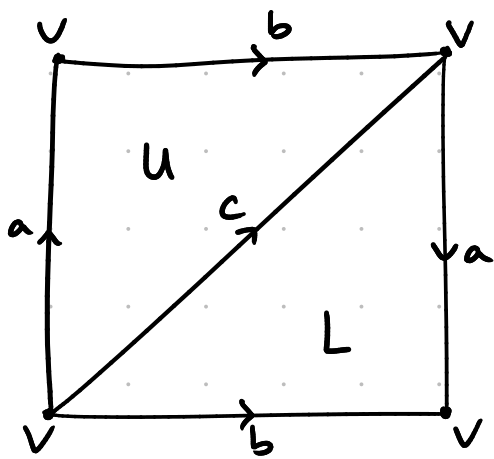
\includegraphics[width=0.2\textwidth]{18_905-201109-1.png}
\end{center}
The chain complex \(S_*(K)\) is
\[
  \begin{tikzcd}
  	\cdots \ar[r] &
  		\ZZ\fgen{U, L} \ar[r] &
  		\ZZ\fgen{a, b, c} \ar[r] &
  		\ZZ\fgen{v} \ar[r] &
  		0 \ar[r] &
  		\cdots
  \end{tikzcd}
\]
To compute the cochain complex \(S^*(K; \FF_2)\),
we have that \(S^0(K; \FF_2) = \ul\Hom(\ZZ\fgen{v}, \FF_2)\).
In particular, a function in \(S^0(K; \FF_2)\) is determined by
where it maps each generator in \(S_0(K)\),
so \(S^0(K; \FF_2) = \FF_2\fgen{\delta_v}\),
where \(\delta_v \colon \ZZ\fgen{v} \to \FF_2\) is
the element corresponding to the generator in the dual vector space.
Similarly, \(S^1(K; \FF_2) = \FF_2\fgen{\delta_a, \delta_b, \delta_c}\), and
\(S^2(K; \FF_2) = \FF_2\fgen{\delta_U, \delta_L}\).
This gives the entire cochain complex \(S^*(K; \FF_2)\):
\[
  \begin{tikzcd}
  	\cdots \ar[r] &
  		\FF_2\fgen{\delta_v} \ar[r, "\partial"] &
  		\FF_2\fgen{\delta_a, \delta_b, \delta_c} \ar[r, "\partial"] &
  		\FF_2\fgen{\delta_U, \delta_L} \ar[r] &
  		0 \ar[r] &
  		\cdots
  \end{tikzcd}
\]

Let's determine what the coboundary morphisms do.
We can use the universal coefficient theorem,
but we will do it manually here.
To calculate \(\partial(\delta_v)\),
note that it is the map \(\ZZ\fgen{a, b, c} \to \FF_2\)
obtained by composing \(\delta_v\) with the boundary map
\(\partial\) in the regular chain complex.
However, note that \(\partial\) maps \(a, b, c \mapsto 0\), so
\(\partial(\delta_v)(a) = \partial(\delta_v)(b) = \partial(\delta_v)(c) = 0\),
and \(\partial(\delta_v) = 0\).

Now let's calculate \(\partial(\delta_a)\),
                    \(\partial(\delta_b)\), and.
In the regular chain complex,
we have \(U \mapsto a + b - c\) and \(L \mapsto c + a - b\).
This gives
\begin{align*}
  \partial(\delta_a)(U) &= \delta_a(a + b - c) = 1 \\
  \partial(\delta_a)(L) &= \delta_a(c + a - b) = 1 \\
  \partial(\delta_b)(U) &= \delta_b(a + b - c) = 1 \\
  \partial(\delta_b)(L) &= \delta_b(c + a - b) = -1 = 1 \\
  \partial(\delta_c)(U) &= \delta_c(a + b - c) = -1 = 1 \\
  \partial(\delta_c)(L) &= \delta_c(c + a - b) = 1.
\end{align*}
Therefore, \(\partial\) maps
\(\delta_a, \delta_b, \delta_c \mapsto \delta_U, \delta_L\).
This gives the cochain complex
\[
  \begin{tikzcd}[row sep=0]
  	\cdots \ar[r] &
  		\FF_2\fgen{\delta_v} \ar[r, "\partial = 0"] &
  		\FF_2\fgen{\delta_a, \delta_b, \delta_c} \ar[r, "\partial"] &
  		\FF_2\fgen{\delta_U, \delta_L} \ar[r] &
  		0 \ar[r] &
  		\cdots \\
  	& & \delta_a \ar[r, mapsto] & \delta_U + \delta_L \\[-0.5ex]
  	& & \delta_b \ar[r, mapsto] & \delta_U + \delta_L \\[-0.5ex]
  	& & \delta_c \ar[r, mapsto] & \delta_U + \delta_L
  \end{tikzcd}
\]

We can then calculate the cohomology:
\begin{align*}
  H^0(K; \FF_2) &\iso \FF_2\fgen{\delta_v} \\
  H^1(K; \FF_2) &\iso \ker \partial
                 \iso \FF_2\fgen{\delta_a + \delta_b, \delta_b + \delta_c} \\
  H^2(K; \FF_2) &= \frac{\FF_2\fgen{\delta_U, \delta_L}}{\delta_U + \delta_L}
                 \iso \FF_2\fgen{k}.
\end{align*}
Let \(\alpha \coloneqq \delta_a + \delta_b\),
    \(\beta \coloneqq \delta_b + \delta_c\), and
    \(k \coloneqq \delta_U\).

We can also compute the cup product structure.
For instance, we can calculate
\(\alpha^2 = (\delta_a + \delta_b)(\delta_a + \delta_b) \in H^2(K; \FF_2)\).
To do this, we determine how it acts on \(U\) and \(L\).
\begin{center}
  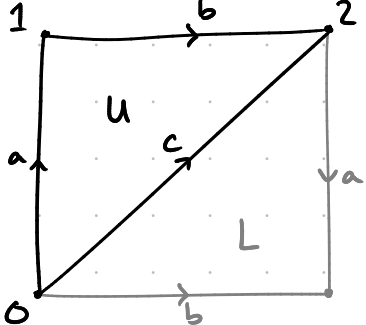
\includegraphics[width=0.2\textwidth]{18_905-201109-2.png}
  \qquad
  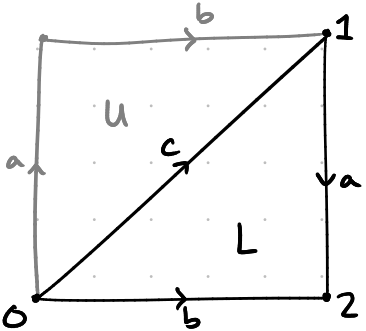
\includegraphics[width=0.2\textwidth]{18_905-201109-3.png}
\end{center}
The front \(1\)-face of \(U\) is \(a\) and
the back \(1\)-face of \(U\) is \(b\).
Therefore,
\[
  \parens[\big]{(\delta_a + \delta_b)(\delta_a + \delta_b)}(U)
    = \parens[\big]{(\delta_a + \delta_b)(a)}
      \parens[\big]{(\delta_a + \delta_b)(b)}
    = (1 + 0)(0 + 1) = 1.
\]
Similarly, the front \(1\)-face of \(U\) is \(a\) and
           the back \(1\)-face of \(U\) is \(b\), so
\[
  \parens[\big]{(\delta_a + \delta_b)(\delta_a + \delta_b)}(L)
    = \parens[\big]{(\delta_a + \delta_b)(c)}
      \parens[\big]{(\delta_a + \delta_b)(a)}
    = (0 + 0)(1 + 0) = 0.
\]
Therefore,
\(\alpha^2 = (\delta_a + \delta_b)(\delta_a + \delta_b) = \delta_U = k\).

Similarly, we can calculate
\begin{align*}
  \parens[\big]{(\delta_b + \delta_c)(\delta_b + \delta_c)}(U)
    &= \parens[\big]{(\delta_b + \delta_c)(a)}
       \parens[\big]{(\delta_b + \delta_c)(b)}
    = (0 + 0)(1 + 0) = 0 \\
  \parens[\big]{(\delta_b + \delta_c)(\delta_b + \delta_c)}(L)
    &= \parens[\big]{(\delta_b + \delta_c)(c)}
       \parens[\big]{(\delta_b + \delta_c)(a)}
    = (0 + 1)(0 + 0) = 0 \\
  \parens[\big]{(\delta_a + \delta_b)(\delta_b + \delta_c)}(U)
    &= \parens[\big]{(\delta_a + \delta_b)(a)}
       \parens[\big]{(\delta_b + \delta_c)(b)}
    = (1 + 0)(1 + 0) = 1 \\
  \parens[\big]{(\delta_a + \delta_b)(\delta_b + \delta_c)}(L)
    &= \parens[\big]{(\delta_a + \delta_b)(c)}
       \parens[\big]{(\delta_b + \delta_c)(a)}
    = (0 + 0)(0 + 0) = 0,
\end{align*}
which means \(\beta^2 = 0\) and \(\alpha\beta = k\).

Therefore, if we consider
\[
  H^*(K; \FF_2)
    \iso \underbracket{\FF_2\fgen{1}}_{\deg 0} \oplus
         \underbracket{\FF_2\fgen{\alpha}
                \oplus \FF_2\fgen{\beta}}_{\deg 1} \oplus
         \underbracket{\FF_2\fgen{k}}_{\deg 2},
\]
we have \(\alpha^2 = \alpha \beta = k\),
        \(\beta^2 = 0\), and
        \(k\alpha = k \beta = k^2 = 0\).
 






\end{document}

\documentclass{standalone}
\usepackage{chez}

\begin{document}
\chapter{November 13, 2020}

For some spaces, cohomology rings are easy to compute.

\begin{example}[\(S^2\)]
  Let's consider \(H^*(S^2; \ZZ)\). This is
  \begin{align*}
    H^*(S^2; \ZZ) &= \bigoplus_p H^p(S^2; \ZZ) \\
      &= \bigoplus_p \ul\Hom_{\cAb}(H_p(S^2), \ZZ) \oplus \Ext(\,\cdot\,).
  \end{align*}
  Since all of the homologies are free, all of the \(\Ext\) terms are zero, so
  \begin{gather*}
    H^0(S^2; \ZZ) \iso \ZZ \\
    H^1(S^2; \ZZ) \iso 0   \\
    H^2(S^2; \ZZ) \iso \ZZ.
  \end{gather*}
  Therefore, \(H^*(S^2; \ZZ) = \underbracket{\ZZ\fgen{1}}_{\deg 0} \oplus
                               \underbracket{\ZZ\fgen{x}}_{\deg 2}\)
  where \(1\cdot x = x \cdot 1 = x\) and \(x^2 = 0\) for degree reasons.
  Therefore, \(H^*(S^2; \ZZ) \iso \ZZ[x]/x^2\).
  We write \(\size x = 2\) to mean that \(x\) is homogeneous of degree \(2\).
\end{example}

In general, for any ring \(R\) and any integer \(n \geq 1\),
\[
  H^*(S^n; R) \iso R[x]/x^2
\]
where \(\size x = n\).
As a module, this is isomorphic to \(R \oplus R\).

\begin{example}[Klein bottle]
  Last time, we saw that
  \[
    H^*(K; \FF_2)
      \iso \underbracket{\FF_2\fgen{1}}_{\deg 0} \oplus
           \underbracket{\FF_2\fgen{\alpha}
                  \oplus \FF_2\fgen{\beta}}_{\deg 1} \oplus
           \underbracket{\FF_2\fgen{k}}_{\deg 2},
  \]
  where \(\alpha^2 = k\), \(\alpha \beta = \beta \alpha = k\), \(\beta^2 = 0\),
  and all other nontrivial products are zero.
  Therefore,
  \[
    H^*(K; \FF_2) \iso \FF_2[\alpha, \beta, k] /
                       (\alpha^2 - k, \beta^2, \alpha\beta - k,
                        \beta\alpha - k, \alpha k, \beta k, k^2).
  \]
\end{example}

\begin{question}
  Is there a continuous map \(S^2 \overset{f}{\to} K\) such that
  \[
    H^2(f; \FF_2)\colon H^2(K; \FF_2) \to H^2(S^2; \FF_2)?
  \]
\end{question}
Note that if \(f \colon S^2 \to J\) exists, it also induces a map of rings
\[
  \begin{tikzcd}[row sep=-1ex]
    H^*(K; \FF_2) \ar[r, "H^*(f)"] & H^*(S^2; \FF_2) \\
    \FF_2[\alpha, \beta, k]/(\alpha\beta - k, \dots) \ar[r] & \FF_2[x]/x^2.
  \end{tikzcd}
\]
Since this is a map of graded rings,
it must send \(\alpha\) and \(\beta\) to \(0\),
because there are no degree \(1\) elements in \(H^*(S^2; \FF_2)\).
Therefore, we must also send \(\alpha^2 = k\) to zero,
so there is no continuous map \(S^2 \to K\).

\begin{adhoctheorem}{Construction}<graded-algebra-product>
  Suppose \(R\) is a ring and \(A^*\), \(B^*\) are two graded \(R\)-algebras.
  Then \(A^* \otimes_R B^*\) has a canonical \(R\)-algebra structure:
  \begin{itemize}[nosep]
    \item \(A^* \otimes_R B^*\) is (obviously) an \(R\)-module.
    \item If \(a \in A^*\) is homogeneous of degree \(p\) and
             \(b \in B^*\) is homogeneous of degree \(q\), then
          \(\size{a \otimes b} = p + q\).
    \item The multiplication is given by
          \[
            (a' \otimes b')(a \otimes b)
              = (-1)^{\size{b'} \size{a}}(a' a \otimes b' b).
          \]
  \end{itemize}
\end{adhoctheorem}

\begin{theorem}
  If \(X, Y \in \cTop\), then the cross product
  \[
    {\times} \colon H^*(X; R) \otimes_R H^*(Y; R) \to H^*(X \times Y; R)
  \]
  is a homomorphism of graded \(R\)-algebras.
\end{theorem}
This is often an isomorphic, in particular when \(H_q(X; R)\) is
a finitely generated free \(R\)-module for all \(q \in \ZZ\).

\begin{proof}
  % see Miller lecture 29
  Suppose \(\alpha_1, \alpha_2 \in H^*(X; R)\) and
          \(\beta_1,  \beta_2  \in H^*(Y; R)\) are homogeneous.
  We need to prove
  \[
    (\alpha_1 \times \beta_1)(\alpha_2 \times \beta_2)
      = (-1)^{\size{\alpha_2} \size{\beta_1}}
        ((\alpha_1 \alpha_2) \times (\beta_1 \beta_2)).
  \]
  Consider
  \[
    \begin{tikzcd}
      X \times Y \ar[rr, "\Delta_{X \times Y}"]
                 \ar[dr, "\Delta_X \times \Delta_Y"'] &&
        X \times Y \times X \times Y \\
      & X \times X \times Y \times Y \ar[ur, "1 \times \text{swap} \times 1"']
    \end{tikzcd}
  \]
  We have
  \begin{align*}
    (\alpha_1 \times \beta_1)(\alpha_2 \times \beta_2)
      &= H^*(\Delta_{X \times Y})
           (\alpha_1 \times \beta_1 \times \alpha_2 \times \beta_2) \\
      &= \parens[\big]{H^*(\Delta_X \times \Delta_Y) \circ
                       H^*(1 \times \text{swap} \times 1)}
           (\alpha_1 \times \beta_1 \times \alpha_2 \times \beta_2) \\
      &= H^*(\Delta_X \times \Delta_Y) \parens[\big]{
           (-1)^{\size{\beta_1} \size{\alpha_2}}
           (\alpha_1 \times \alpha_2 \times \beta_1 \times \beta_2)} \\
      &= (-1)^{\size{\beta_1} \size{\alpha_2}}
           ((\alpha_1 \alpha_2) \times (\beta_1 \beta_2)). \pog
  \end{align*}
\end{proof}

\begin{example}
  Suppose we want to calculate \(H^*(T^2; \ZZ)\).
  Note that we have \(T^2 = S^1 \times S^1\).
  First, note that
  \[
    \times \colon H^*(S^1; \ZZ) \otimes_\ZZ H^*(S^1; \ZZ) \to
                  H^*(S^1 \times S^1; \ZZ)
  \]
  is an isomorphism.
  If we let the two copies of \(H^*(S^1; \ZZ)\) be
    \(\ZZ\fgen{1} \oplus \ZZ\fgen{a}\), \(\size a = 1\), \(a^2 = 0\) and
    \(\ZZ\fgen{1} \oplus \ZZ\fgen{b}\), \(\size b = 1\), \(b^2 = 0\),
  then
  \[
    H^*(S^1; Z) \otimes_\ZZ H^*(S^1; Z)
      \iso \underbracket{\ZZ\fgen{1 \otimes 1}}_{\deg 0} \oplus
           \underbracket{\ZZ\fgen{a \otimes 1} \oplus
                         \ZZ\fgen{1 \otimes b}}_{\deg 1} \oplus
           \underbracket{\ZZ\fgen{a \otimes b}}_{\deg 2}.
  \]
  The only interesting tensor products are
  the ones between degree \(1\) elements.
  We have
  \begin{align*}
    (a \otimes 1) (1 \otimes b)
      &= (-1)^{0 \cdot 0} (a 1 \otimes 1 b) = a \otimes b \\
    (1 \otimes b) (a \otimes 1)
      &= (-1)^{1 \cdot 1} (1 a \otimes b 1) = -(a \otimes b) \\
    (a \otimes 1) (a \otimes 1)
      &= (-1)^{0 \cdot 1} (a a \otimes 1 1) = (0 \otimes 1) = 0 \\
    (1 \otimes b) (1 \otimes b)
      &= (-1)^{1 \cdot 0} (1 1 \otimes b b) = (1 \otimes 0) = 0.
  \end{align*}
  If we let \(x = a \otimes 1\), \(y = 1 \otimes b\), and \(z = a \otimes b\),
  we get
  \[
    H^*(T^2; \ZZ) \iso \ZZ[x, y, z]/(xy - z, x^2, y^2, xz, yz, z^2).
  \]

  One trick we could have used to compute \(x^2\) is
  \[
    x^2 = x \cdot x = (-1)^1 x \cdot x \implies 2x^2 = 0 \implies x^2 = 0.
  \]
\end{example}














\end{document}

\documentclass{standalone}
\usepackage{chez}

\begin{document}
\chapter{November 16, 2020}

Recall that if \(A^*\) and \(B^*\) are graded \(R\)-algebras, then
\(A^* \oplus B^*\) is also a graded algebra with multiplication given by
\((a, b)(a', b') = (aa', bb')\), with unit \((1, 1)\).

\begin{remark}
  This direct sum is the product of \(A^*\) and \(B^*\) in
  the category of graded \(R\)-modules.
\end{remark}

\begin{proposition}
  Suppose \(X\) and \(Y\) are topological spaces. Then
  \(H^*(X \amalg Y; R) \iso H^*(X; R) \oplus H^*(Y; R)\)
  as \(R\)-algebras.
\end{proposition}
\begin{proof}
  The inclusions \(X \hookrightarrow X \amalg Y\) and
                 \(X \hookrightarrow X \amalg Y\) induce maps
                 of graded \(R\)-algebras:
  \begin{gather*}
    H^*(X \amalg Y; R) \to H^*(X; R) \\
    H^*(X \amalg Y; R) \to H^*(Y; R).
  \end{gather*}
  This induces a map, by the universal property of a product in a category
  \[
    H^*(X \amalg Y; R) \to H^*(X; R) \oplus H(Y; R).
  \]
  This is automatically a map of graded \(R\)-algebras.
  To prove it is an isomorphism, we need to just check that it
  is an isomorphism of abelian groups.
\end{proof}



\subsection{Cohomology of wedge products}
Suppose \(X\) is a topological space with \(x \in X\), and
        \(Y\) is a topological space with \(y \in Y\).
Then recall that \(X \vee Y = X \amalg Y / (x \sim y)\).
Note that there is a quotient map
\[
  r \colon X \amalg Y \to X \vee Y.
\]
Using the long exact sequence of a pair, % ???
we see that \(H_q(X \amalg Y) \to H_q(X \vee Y)\)
is an isomorphism for \(q > 0\).
By the universal coefficient theorem,
\[
  H^q(X \vee Y; R) \to H^q(X \amalg Y; R)
\]
is also an isomorphism.

\begin{corollary}
  The quotient map
  \[
    X \amalg Y \overset{r}{\to} X \vee Y
  \]
  induces a map of graded \(R\)-algebras
  \[
    H^*(X \vee Y) \to H^*(X \amalg Y)
  \]
  which is an isomorphism in positive degrees.
\end{corollary}
In degree \(0\), it is an injection.

\begin{example}
  Consider \(S^2 \vee S^1 \vee S^1\).
  The cohomology ring \(H^*(S^2 \vee S^1 \vee S^1; \ZZ)\) injects into
  \[
    H^*(S^2; \ZZ) \oplus
    H^*(S^1; \ZZ) \oplus
    H^*(S^1; \ZZ)
  \]
  that is an isomorphism in positive degrees,
  and an injection in degree \(0\).
  In particular, the cohomology ring injects into
  \[
    \underbracket{\ZZ \oplus \ZZ \oplus \ZZ}_{\deg 0} \oplus
    \underbracket{\ZZ \oplus \ZZ}_{\deg 1} \oplus
    \underbracket{\ZZ \oplus}_{\deg 2},
  \]
  where the degree \(0\) component is generated by
    \((1_{S^2}, 0, 0)\), \((0, 1_{S^1}, 0)\), and \((0, 0, 1_{S^1})\);
  the degree \(1\) component is generated by
    \((0, x, 0)\) and \((0, 0, x)\); and
  the degree \(2\) component is generated by
    \((y, 0, 0)\),
  where \(x \in H^1(S^1; \ZZ)\) and \(y \in H^2(S^2; \ZZ)\) are generators.

  Then \(H^*(S^2 \vee S^1 \vee S^1; \ZZ)\) is the subring generated by
  \[
    \underbracket{(1_{S^2}, 1_{S^2}, 1_{S^2})}_{\deg 0},
    \underbracket{(0, x, 0),
                  (0, 0, x)}_{\deg 1},
    \underbracket{(y, 0, 0)}_{\deg 2},
  \]
  i.e.\
  \[
    H^*(S^2 \vee S^1 \vee S^1; \ZZ)
      \iso \ZZ \oplus \ZZ \oplus \ZZ \oplus \ZZ.
  \]
  All products of positive degree classes are trivial.
\end{example}

\begin{question}
  Is \(S^2 \vee S^1 \vee S^1\) homotopy equivalent to the torus \(T^2\)?
  Note that \(H_q(S^2 \vee S^1 \vee S^1; \ZZ) \iso H_q(T; \ZZ)\)
  for all \(q\).

  However, the cohomology ring of \(S^2 \vee S^1 \vee S^1\)
  has trivial positive degree products,
  but the cohomology ring of \(T^2\) is
  \(\ZZ[x, y, z]/(x^2, y^2, xy-z, z^2, xz, yz)\).
  In particular, \(xy = z\), even though \(x\) and \(y\) are both
  in positive degrees.

  Therefore, these spaces are not homotopy equivalent, or in other words
  \[
    S^2 \vee S^1 \vee S^1 \ncong T^2
  \]
  in \(\cHoTop\).
  Another way to think about this is that the diagonal maps
  \begin{gather*}
    (S^2 \vee S^1 \vee S^1) \to
      (S^2 \vee S^1 \vee S^1) \times (S^2 \vee S^1 \vee S^1) \\
    T^2 \to T^2 \times T^2
  \end{gather*}
  induce different maps in homology.
\end{question}


\section{Poincar\'e duality}
Suppose \(A\) is an abelian group and \(R\) is a ring.
Then there is a map
\[
  \ul\Hom_{\cAb}(A, R) \otimes_\ZZ A \overset{f}{\to} R
\]
adjoint, under the currying isomorphism, to the identity
\[
  \ul\Hom_\cAb(A, R) \overset{g}{\to}
  \ul\Hom_\cAb(A, R).
\]
In particular, this is the evaluation map
\(\varphi \otimes m \mapsto \varphi(m)\).

Similarly, if \(M\) is an \(R\)-module, there is a map
\[
  \ul\Hom_\cRmod(M, R) \otimes_R M \overset{f}{\to} R
\]
adjoint to the identity
\[
  \ul\Hom_\cRmod(M, R) \to \ul\Hom_\cRmod(M, R).
\]

\subsection{Kronecker pairing}
Suppose \(X\) is a topological space and \(R\) is a ring.
Then there is a pairing map
\[
  \angles{{-}, {-}} \colon H^q(X; R) \otimes_R H_q(X; R) \to R.
\]

To see this, note that a class in \(H^q(X; R)\) is represented by
a cocycle in \(S^q(X; R)\) modulo coboundaries,
i.e.\ functions \(\Sing_q(X) \to R\).
A class in \(H^q(X; R)\) is represented by
a formal \(R\)-linear combination of classes in \(\Sing_q(X)\),
which are cycles modulo boundaries.

We can take any function \(\Sing_q(X) \to R\) and evaluate it on
any formal \(R\)-linear combination of classes in \(\Sing_q(X)\).
In other words, we have a map
\[
  S^q(X; R) \otimes_R S_q(X; R) \to R,
\]
which extends to a chain map
\[
  S^*(X; R) \otimes_R S_*(X; R) \to R,
\]
or a map
\[
  H^*(X; R) \otimes_R H_*(X; R) \to R.
\]













\end{document}

\documentclass{standalone}
\usepackage{chez}

\begin{document}
\chapter{November 18, 2020}

\begin{proposition}[Problem 1 of PSET]<homology-cohomology-pairing>
  If \(X\) is a finite type CW complex, then the map,
  adjoint to the Kronecker pairing
  \[
    H^q(X; \FF_2)
      \to \ul\Hom_{\FF_2\text{-}\cat{mod}}(H_q(X; \FF_2), \FF_2) % chktex 35
  \]
  is an isomorphism.
\end{proposition}
This is an example of a perfect pairing.

\begin{definition}
  A \vocab{perfect pairing} of two finitely generated free \(R\)-modules
  \(V\) and \(W\) is an \(R\)-linear map
  \[
    V \otimes_R W \to R
  \]
  such that the adjoint map
  \[
    V \to \ul\Hom_R(W, R)
  \]
  is an isomorphism of \(R\) modules.
\end{definition}

\begin{definition}
  An \(n\)-dimensional \vocab{manifold} \(M\) is a Hausdorff topological space
  such that every point has an open neighborhood homeomorphic to \(\RR^n\).
\end{definition}

\begin{example}
  A \(2\)-dimensional manifold is called a \vocab{surface}.
  Examples include \(S^2\),
                   \(T^2\),
                   the Klein bottle \(K\),
                   \(\RP^2\), and
                   \(\RR^2\).
  
  Non-examples include \(S^2 \vee S^2\), because at the wedge point,
  there is no open neighborhood homeomorphic to \(\RR^2\).

  Examples of 3D manifolds include \(\RR^3\),
                                   \(S^3\),
                                   \(S^1 \times S^1 \times S^1\),
                                   \(\RP^3\), etc.

  Other manifolds include
  \begin{itemize}[nosep]
    \item smooth algebraic varieties over \(\RR\) or \(\CC\),
    \item configuration spaces in physics.
  \end{itemize}
\end{example}

\begin{fact}
  Any compact manifold is homotopy equivalent to a finite type CW complex.
\end{fact}


\begin{theorem}[Poincar\'e duality]
  Let \(M\) be a compact \(n\)-dimensional manifold.
  Then there exists a unique class \([M] \in H_n(M; \FF_2)\)
  called the \vocab{fundamental class} of the manifold, such that
  for all \(p, q \in \ZZ\) such that \(p + q = n\), the map
  \[
    H^p(M; \FF_2) \otimes_{\FF_2} H^q(M; \FF_2) \xrightarrow{\cup}
      H^n(M; \FF_2) \xrightarrow{\angles{{-}, [M]}} \FF_2
  \]
  is a perfect pairing.
\end{theorem}
In other words, \(H^p(M; \FF_2)\) is canonically isomorphic to
the \(F_2\)-linear dual of \(H^q(M; \FF_2)\).

\begin{example}
  Suppose \(M\) is a compact 3D manifold with
  \(H^0(M; \FF_2) = \FF_2 \oplus \FF_2\) and
  \(H^1(M; \FF_2) = \FF_2 \oplus \FF_2 \oplus \FF_2\).
  Then we can determine \emph{all} of
  the homology and cohomology groups of \(M\) with \(\FF_2\) coefficients.
  In particular,
  \begin{align*}
    H^2(M; \FF_2) &\iso \ul\Hom(H^1(M; \FF_2), \FF_2)
                   \iso \FF_2 \oplus \FF_2 \oplus \FF_2 \\
    H^3(M; \FF_2) &\iso \ul\Hom(H^0(M; \FF_2), \FF_2)
                   \iso \FF_2 \oplus \FF_2,
  \end{align*}
  and all other cohomology groups vanish.
  All other cohomology groups vanish, because e.g.\
  \[
    H^4(M; \FF_2) \iso H^{-1}(M; \FF_2)^\vee \iso 0^\vee \iso 0.
  \]

  From \cref{prop:homology-cohomology-pairing}, we have
  \begin{align*}
    H_0(M; \FF_2) &\iso \FF_2 \oplus \FF_2 \\
    H_1(M; \FF_2) &\iso \FF_2 \oplus \FF_2 \oplus \FF_2 \\
    H_2(M; \FF_2) &\iso \FF_2 \oplus \FF_2 \oplus \FF_2 \\
    H_3(M; \FF_2) &\iso \FF_2 \oplus \FF_2,
  \end{align*}
  and \(H_q(M; \FF_2) \iso 0\) for \(q > 3\).
\end{example}


\begin{example}
  Recall
  \begin{align*}
    H^*(T^2; \FF_2) &= \FF_2[x, y, z]/(xy - z, x^2, y^2, xz, yz, z^2) \\
      &\iso \underbracket{\FF_2\fgen{1}}_{\deg 0} \oplus
            \underbracket{\FF_2\fgen{x, y}}_{\deg 1} \oplus
            \underbracket{\FF_2\fgen{z}}_{\deg 2}.
  \end{align*}
  The fundamental class of the torus is
  an element of \(H_2(T^2; \FF_2) \iso \FF_2\fgen{\delta_z}\).
  The fundamental class is \(\delta_z\).

  By Poincar\'e duality, there is a perfect pairing
  \[
    P \colon H^1(T^2; \FF_2) \otimes_{\FF_2} H^1(T^2; \FF_2) \to \FF_2
  \]
  where
  \begin{align*}
    P(x \otimes y) &= \angles{xy, \delta_z}
                    = \angles{z, \delta_z}
                    = \delta_z(z) = 1 \\
    P(x \otimes x) &= \angles{xx, \delta_z}
                    = \angles{0, \delta_z}
                    = \delta_z(0) = 0,
  \end{align*}
  etc.

  There is another pairing
  \[
    P \colon H^0(T^2; \FF_2) \otimes_{\FF_2} H^2(T^2; \FF_2) \to \FF_2
  \]
  where
  \[
    P(1 \otimes z) = \angles{1z, \delta_z}
                   = \angles{z, \delta_z}
                   = \delta_z(z) = 1.
  \]
\end{example}

\begin{example}
  What is \(H^*(\RP^2; \FF_2)\)?
  Note that \(\RP^2\) is a 2D compact manifold.
  We can compute
  \begin{gather*}
    H^0(\RP^2; \FF_2) \iso \FF_2 \\
    H^1(\RP^2; \FF_2) \iso \FF_2
  \end{gather*}
  because \(\RP^2\) has one path component.
  For \(H^1\), we have to manually calculate it.
  However, for \(H^2\), we can use Poincar\'e duality, which gives
  \[
    H^2(\RP^2; \FF_2) \iso H^0(\RP^2; \FF_2) \iso \FF_2.
  \]
  Therefore, we can write
  \[
    H^*(\RP^2; \FF_2) \iso \underbracket{\FF_2\fgen{1}}_{\deg 0} \oplus
                           \underbracket{\FF_2\fgen{a}}_{\deg 1} \oplus
                           \underbracket{\FF_2\fgen{b}}_{\deg 2}.
  \]
  We know that \(b^2 = ab = 0\) for degree reasons, so the only question is
  if \(a^2 = b\) or \(a^2 = 0\).

  There is a perfect pairing
  \[
    P \colon H^1(\RP^2; \FF_2) \otimes_{\FF_2} H^1(\RP^2; \FF_2) \to \FF_2.
  \]
  This map must be nontrivial in order for its adjoint to be an isomorphism.
  Therefore, \(P(a \otimes a) = \angles{a^2, [\RP^2]} \neq 0\), so
  \(a^2 \neq 0\), and furthermore \(a^2 = b\).

  Therefore,
  \[
    H^*(\RP^2; \FF_2) \iso \FF_2[a, b]/(a^2 - b, ab, b^2),
  \]
  where \(\size a = 1\) and \(\size b = 2\).
\end{example}

\begin{remark}
  Note that
  \(H^*(S^2 \vee S^1; \FF_2) \iso \FF_2[a, b]/(a^2, ab, b^2)\)
  where \(\size a = 1\) and \(\size b = 2\).
  So the cohomology groups are the same as \(\RP^2\),
  but the ring structure is different.

  In particular, \(S^2 \vee S^1\) is not a manifold,
  so we cannot apply Poincar\'e duality.
\end{remark}






\end{document}

\documentclass{standalone}
\usepackage{chez}

\begin{document}
\chapter{November 20, 2020}
\subsection{Geometric intuition of Poincar\'e duality}
Consider the torus \(T^2\) with the two standard loops:
\begin{center}
  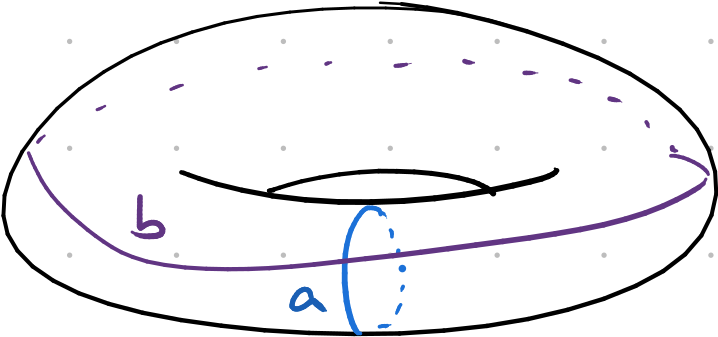
\includegraphics[width=0.27\textwidth]{18_905-201120-1.png}
\end{center}
The loops \(a\) and \(b\) are geometric pictures of cycles
representing generators of \(H_q(T; \FF_2) \iso \FF_2\fgen{a,b}\).

\begin{center}
  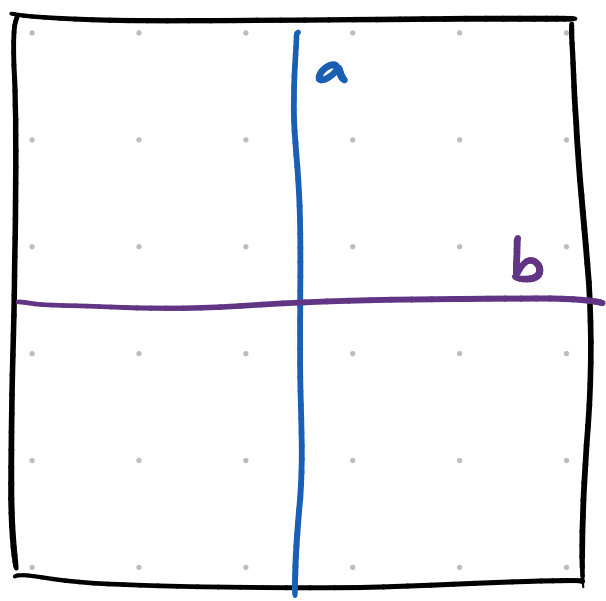
\includegraphics[width=0.18\textwidth]{18_905-201120-2.png}
  \qquad
  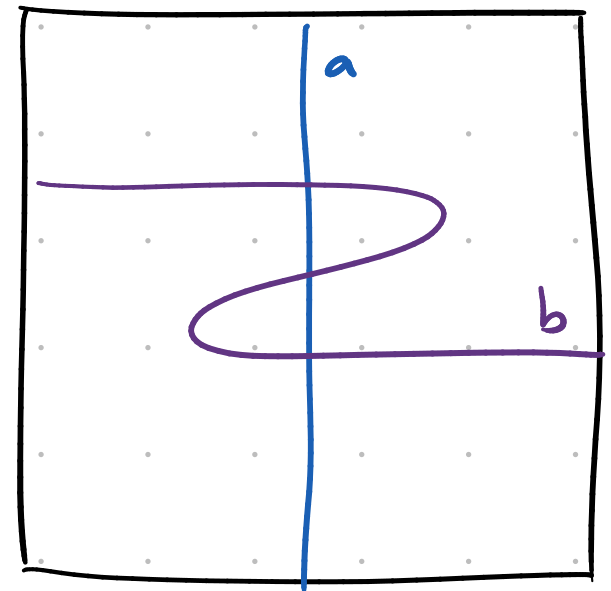
\includegraphics[width=0.18\textwidth]{18_905-201120-3.png}
\end{center}
How many times do \(a\) and \(b\) intersect modulo \(2\)?
No matter how we deform \(a\) and \(b\),
they will intersect an odd number of times.

In very special configurations, they intersect an even number of times.
\begin{center}
  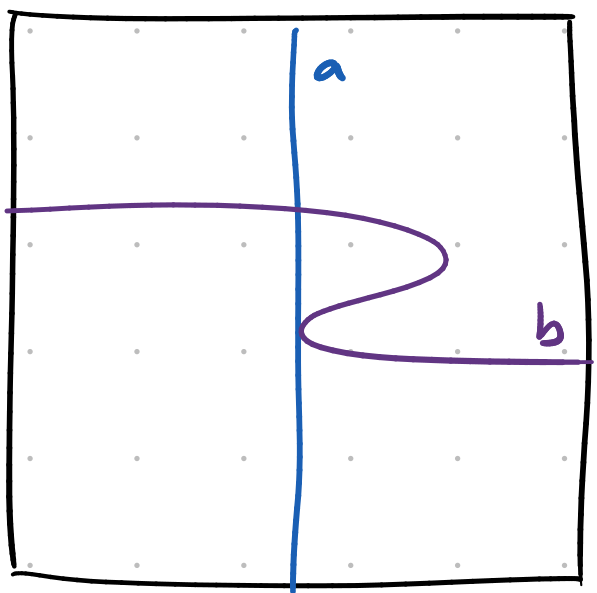
\includegraphics[width=0.18\textwidth]{18_905-201120-4.png}
\end{center}
However, this situation is unstable, i.e.\ deforming \(a\) or \(b\) slightly
will return to an odd number of intersections.

In a class on smooth manifolds, one could prove that the first two pictures
involve \vocab{transverse} interactions, while the last one involves
not transverse interactions.
In order to do this, we would need to go into smooth geometry,
where we can talk about tangent lines.
However, we can use the cup product to talk about these intersections.
In particular, this is a purely topological structure
that does not care about geometry.

We can ask stranger things such as: How many times does \(a\) intersect \(a\)?
We should think about this by thinking about \(a\) as a generic representative
for its homology.
\begin{center}
  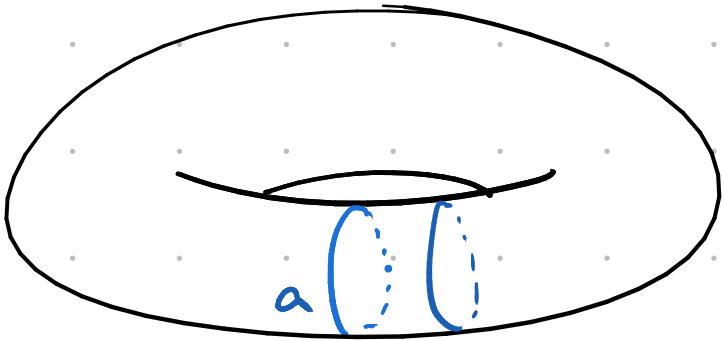
\includegraphics[width=0.2\textwidth]{18_905-201120-5.png}
  \qquad
  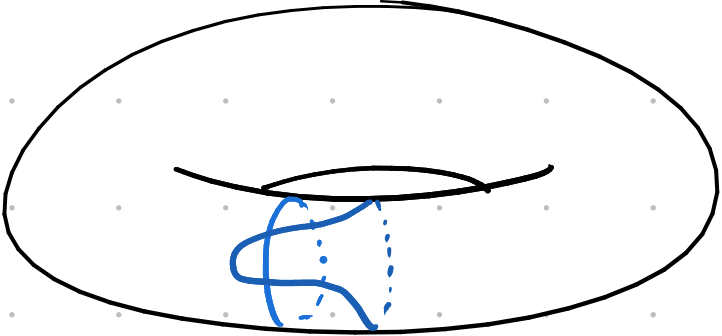
\includegraphics[width=0.2\textwidth]{18_905-201120-6.png}
\end{center}
We can see that generically, \(a\) will intersect \(a\)
an even number of times.

We can define an \(\FF_2\)-module homomorphism
\[
  f_a \colon H_1(R; \FF_2) \iso \FF_2\fgen{a, b} \to \FF_2
\]
which sends \(a \mapsto 0\) and \(b \mapsto 1\),
i.e.\ it counts the number of intersections with \(a\) modulo \(2\).

Using the isomorphism
\[
  H^1(T; \FF_2)
    \iso \ul\Hom_{\FF_2\text{-}\cat{mod}}(H_1(T, \FF_2), \FF_2), % chktex 35
\]
we get that \(f_a\) represents a class in \(H^1(T; \FF_2)\),
which is the \vocab{Poincar\'e dual} of \(a\).


In general, suppose \(M\) is a compact \(n\)-dimensional manifold
where \(p\) and \(q\) are integers such that \(p + q = n\).
If we fix a cycle \(a \in H_p(M; \FF_2)\),
this represents a \(p\)-dimensional submanifold of \(M\).
For any \(b \in H_q(M; \FF_2)\),
\(a\) and \(b\) will intersect at some number
of points, since the dimensions are complementary.
It turns out that the number of points modulo \(2\) is independent
of the generic geometric representatives we chose for \(a\) and \(b\).

Overall, if we fix \(a \in H_p(M; \FF_2)\) and vary \(b \in H_q(M; \FF_2)\),
we get a function
\[
  f_a \colon H_q(M; \FF_2) \to \FF_2,
\]
which can be viewed as a class in \(H^q(M; \FF_2)\).
The Poincar\'e duality theorem says that this defines an isomorphism
\begin{align*}
  H_p(M; \FF_2) &\iso H^q(M; \FF_2) \\[-1ex]
    a &\mapsto f_a.
\end{align*}
In particular, this states a cycle, modulo boundaries,
is determined by the number of times it intersects all other cycles
in complementary dimension.


Last time, we had the perfect pairing
\begin{align*}
  P \colon& H^q(X; \FF_2) \otimes H^p(X; \FF_2) \to \FF_2 \\[-1ex]
    & u \otimes v \mapsto \angles{uv, [M]}
\end{align*}
which induces an isomorphism
\begin{align*}
  H^q(M; \FF_2)
    &\iso \ul\Hom_{\FF_2\text{-}\cat{mod}}(H^p(X; \FF_2), \FF_2) \\ % chktex 35
    &\iso H_p(X; \FF_2).
\end{align*}

\begin{claim}
  These two isomorphisms are equivalent.
\end{claim}

\begin{remark}
  The fundamental class \([M] \in H_n(M; \FF_2)\) is Poincar\'e dual to
  \(1 \in H^0(M; \FF_2) \subseteq H^*(M; \FF_2)\),
  the function that takes every path component to \(1\).
  Geometrically, this is the class that covers the whole manifold
  if we think about intersections.
\end{remark}

There is also a version of Poincar\'e duality with integer coefficients,
but it's more complicated and only works for oriented manifold.
The idea is as follows:

Consider the torus \(T^2\), which will be oriented,
and the loops \(a\) and \(b\) from before,
where they intersect three times and we give them directions.
In particular, consider the diagram with three intersections,
and zoom into the three intersections.
\begin{center}
  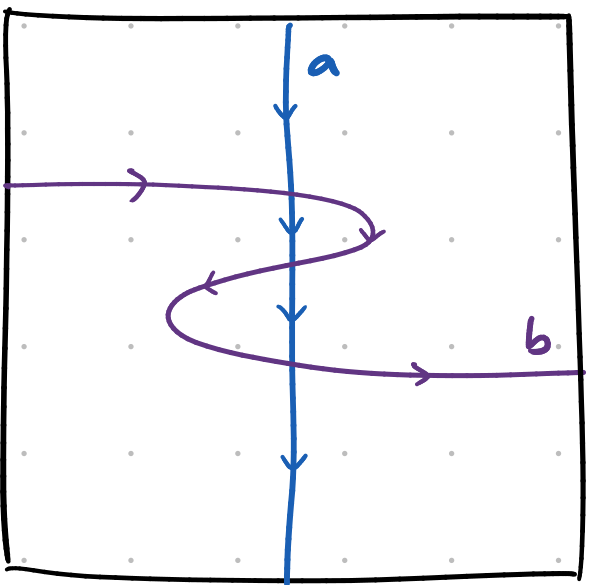
\includegraphics[width=0.22\textwidth, align=c]{18_905-201120-7.png}
  \qquad
  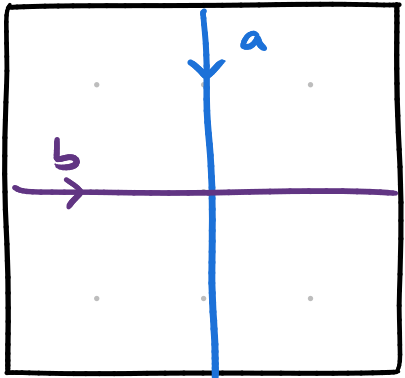
\includegraphics[width=0.18\textwidth, align=c]{18_905-201120-8.png}
  \qquad
  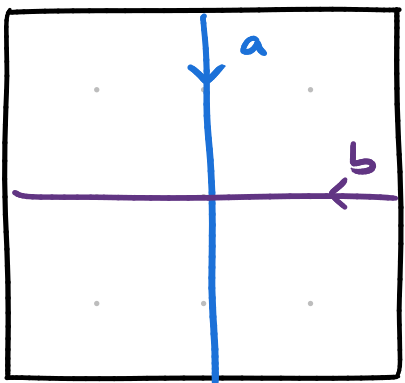
\includegraphics[width=0.18\textwidth, align=c]{18_905-201120-9.png}
  \qquad
  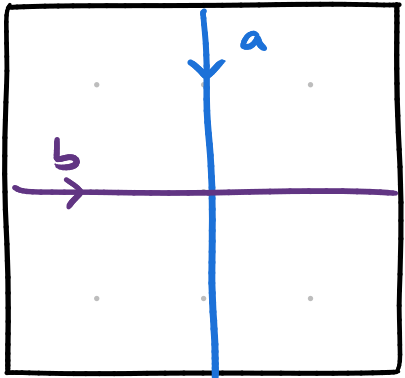
\includegraphics[width=0.18\textwidth, align=c]{18_905-201120-8.png}
\end{center}
The idea is that the last two diagrams differ by a reflection,
and when we count intersections, we do a signed count,
where a reflection introduces a minus sign.
Therefore, the last two diagrams cancel each other out,
and there is only one signed intersection.

However, this only works for oriented manifolds because
for nonoriented manifolds, going around in a loop might cause
the diagrams to be inconsistent, i.e.\ they will become reflected.

\section{More applications of Poincar\'e duality}
Last time, we computed \(H^*(\RP^2; \FF_2) \iso \FF_2[a]/a^3\).
But more generally, we can compute \(H^*(\RP^n; \FF_2)\).
\begin{example}[\(H^*(\RP^3; \FF_2)\)]
  As a graded vector space, we have
  \[
    H^*(\RP^3; \FF_2)
      \iso \underbracket{\FF_2\fgen{1}}_{\deg 0} \oplus
           \underbracket{\FF_2\fgen{a}}_{\deg 1} \oplus
           \underbracket{\FF_2\fgen{b}}_{\deg 2} \oplus
           \underbracket{\FF_2\fgen{c}}_{\deg 3}.
  \]
  In particular, we have the perfect pairing
  \[
    P \colon
      H^1(\RP^2) \otimes_{\FF_2} H^2(\RP^2) \iso \FF_2\fgen{a \otimes b}
      \to \FF_2
  \]
  where \(P(a \otimes b) = \angles{ab, [\RP^3]}\).
  In particular, this is a nontrivial map \(\FF_2 \to \FF_2\),
  so \(ab \neq 0\), and furthermore \(ab = c\).

  We can completely determine \(H^*(\RP^n; \FF_2) \iso \FF_2[a]/a^{n+1}\)
  where \(\size a = 1\).
\end{example}


\begin{theorem}[Borsuk-Ulam]
  Let \(f \colon S^n \to \RR^n\) be a continuous function.
  There exists \(x \in S^n\) such that \(f(x) = f(-x)\).
\end{theorem}
\begin{example}
  At any moment in time, some antipodal pair of points on Earth
  share the same temperature and air pressure.
\end{example}
\begin{proof}
  Suppose no such \(x\) exists.
  Consider
  \begin{align*}
    g \colon& S^n \to S^{n-1} \\[-1ex]
      & x \mapsto \frac{f(x) - f(-x)}{\abs{f(x) - f(-x)}}.
  \end{align*}
  This is well defined because the denominator is never zero.
  Note that \(g(-x) = -g(x)\).
  Hence, there is a continuous map \(\bar g \colon \RP^n \to \RP^{n-1}\)
  induced by \(g\).

  We claim that the map
  \[
    H_1(\bar g; \FF_2) \colon H_1(\RP^n; \FF_2) \iso \FF_2
                            \to H_1(\RP^{n-1}; \FF_2) \iso \FF_2
  \]
is nontrivial.
Consider the path in \(S^n\) going from the north pole to the south pole.
Upon projection to \(\RP^n\), this becomes a cycle that generates
\(H_1(\RP^n; \FF_2)\).
Mapping under \(\bar g\) gives a nontrivial element of
\(H_1(\RP^{n-1}; \FF_2)\).

We now proceed with the remainder of the proof.
By Poincar\'e duality, we have that \(H^1(\bar g; \FF_2)\) is nontrivial.
In particular, the following map must satisfy
\begin{align*}
  H^*(\bar g; \FF_2) \colon& H^*(\RP^{n-1}; \FF_2) \to
                             H^*(\RP^{n}; \FF_2) \\[-1ex]
    \colon& \FF_2[a]/a^n \to \FF_2[a]a^{n+!} \\[-1ex]
    & a \mapsto a,
\end{align*}
but there is no such ring map, which is a contradiction.
\end{proof}


\end{document}

\documentclass{standalone}
\usepackage{chez}

\begin{document}
\chapter{December 02, 2020}
\section{Proof of Poincar\'e duality}
\subsection{Constructions}
So far, we have the constructions relating homology and cohomology:
\begin{description}
  \item[Cross products]
  \[
    \times \colon H^p(X; R) \otimes_R H^q(Y; R) \to H^{p+q}(X \times Y; R)
  \]
  
  \item[Cup products]
  \[
    \times \colon H^p(X; R) \otimes_R H^q(X; R) \to H^{p+q}(X \times X; R),
  \]
  which is the cross product combined with the diagonal map.

  \item[Kronecker pairing]
  \[
    H^p(X; R) \otimes_R H_p(X; R) \to R,
  \]
  which is taking some function on homology
  (i.e.\ and element of cohomology)
  and evaluating it.
\end{description}

\begin{definition}
  The \vocab{cap product} is the operation
  \[
    \cap \colon H^p(X; R) \otimes_R H_n(X; R) \to H_{n-p}(X; R).
  \]
  is defined by applying homology to the chain map
  \[
    S^p(X; R) \otimes_R S_n(X; R) \xrightarrow{\mathrm{AW}}
    S^p(X; R) \otimes_R S_p(X; R) \otimes_R S_{n-p}(X; R)
    \xrightarrow{\angles{-, -}} R \otimes_R S_{n-p}(X; R) \iso S_{n-p}(X; R),
  \]
  where \(\mathrm{AW}\) is the Alexander-Whitney map.
\end{definition}
This is a variation of the Kronecker pairing that doesn't require
the elements to come from a homology and cohomology of the same degree.

\begin{note}
  All of these constructions come from
  \begin{itemize}[nosep]
    \item the cross product,
    \item the diagonal map on a space, and
    \item the Kronecker pairing.
  \end{itemize}
\end{note}
Here are some properties of the cap product:
\begin{enumerate}
  \item \((a \cup b) \cap x = a \cap (b \cap x)\) and \(1 \cap x = x\).
    In other words, \(H_*(X; R)\) is a module for \(H^*(X; R)\).
  \item \(\angles{a \cup b, x} = \angles{a, b \cap x}\).
  \item Let \(\eps \colon H_0(X; R) \to R\) be
    the element adjoint to \(1 \in H^0(X; R)\).
    Then if \(b \in H^p(X; R)\) and \(x \in H_p(X; R)\), then
    \[
      \eps(b \cap x) = \angles{b, x}.
    \]
  \item(Projection formula) Given a map \(f \colon X \to Y\),
                                        \(b \in H^p(Y)\), and
                                        \(x \in H_n(X)\),
    \[
      H_*(f)(H^*(f)(b) \cap x) = b \cap (H_*(f)(x)).
    \]
\end{enumerate}

\begin{theorem}[Poincar\'e duality]
  Let \(M\) be a compact \(n\)-dimensional manifold
  equipped with an \(R\)-orientation for a PID \(R\).
  Then there is a unique \([M] \in H_n(M; R)\) that
  restricts to the local orientation in \(H_n(M; M - \set{x}) \otimes_\ZZ R\)
  for each point \(x \in M\), such that
  \begin{align*}
    H^p(M; R) &\to H_{n-p}(M; R) \\[-1ex]
      a &\mapsto a \cap [M]
  \end{align*}
  is an isomorphism for all \(p \in \ZZ\).
\end{theorem}
To understand this geometrically, consider the reverse map.
It takes a homology class and records the function on \(p\)th homology
that counts intersections with sign depending on the \(R\)-orientation
around each intersection.

We will prove this with \(R = \ZZ\) for the notation simplicity.
The more general proof is not any harder.
We will prove Poincar\'e duality by formulating
a more general statement that works for
compact subsets of arbitrary manifolds.

\subsection{Relative cap products}
Suppose \(A \subseteq X\) is a subspace of \(X\).
Then there is a \vocab{relative cap product}
\[
  H^p(X) \otimes H_n(X, A) \to H_{n-p}(X, A)
\]
making \(H_*(X, A)\) a module over \(H^*(X)\).
This is constructed via the following diagram.
\[
  \begin{tikzcd}[column sep=small]
    0 \ar[d] && 0 \ar[d] \\
    S^p(X) \otimes S_n(A) \ar[r] \ar[d] &
      S^p(A) \otimes S_n(A) \ar[r, "\cap"] &
      S_{n-p}(A) \ar[d] \\
    S^p(X) \otimes S_n(X) \ar[rr, "\cap"] \ar[d] &&
      S_{n-p}(X) \ar[d] \\
    S^p(X) \otimes S_n(X, A) \ar[rr, dashed] \ar[d] &&
      S_{n-p}(X, A) \ar[d] \\
    0 && 0
  \end{tikzcd}
\]
We have a short exact sequence of chain complexes on the left
from the definition of \(S_n(X, A) \iso S_n(X / A)\).
We then have the map \(S^p(X) \otimes S_n(A) \to S^p(A) \otimes S_n(A)\)
from the inclusion \(A \subseteq X\).
Then, the rectangle commutes by the projection formula.
Then, the dashed arrow exists by the universal property of a quotient.
Taking the homology of the dashed arrow gives the relative cap product.

\subsection{\v{C}ech cohomology}
Suppose \(K \subseteq X\) is a closed subset of a topological space \(X\).
By excision, we have
\[
  H_n(X, X-K) \iso H_n(U, U-K)
\]
for any open \(U\) containing \(K\).
Note that we have a relative cap product
\[
  H^p(U) \otimes H_n(U, U-K) \to H_{n-k}(U, U-K).
\]
Thus, \(H_*(X, X-K)\) is a module over \(H^*(U)\)
for every open \(U\) containing \(K\).

\begin{definition}
  The \(p\)th \vocab{\v{C}ech cohomology} of \(K\)
  is denoted \(\check{H}^p(K)\).
  An element \(x \in \check{H}^p(K)\) is an element of \(H^p(U)\)
  for some open \(U\) containing \(K\).
  If \(K \subseteq U \overset{}\subseteq V\), we let
  \(x \in H^p(V) \subseteq \check{H}^p(X)\) be equal to
  \[
    H^*(i)(x) \in H^p(U) \subseteq H^p(X).
  \]
\end{definition}
Informally, this tries to capture the cohomology rings of
arbitrarily small open subsets of \(K\).

\begin{remark}
  \(\check{H}^p(K)\) depends on how \(K\) sits in \(X\).
  For ``reasonable'' \(K \subseteq X\),
  we have \(\check{H}^*(K) \iso H^*(K)\),
  but this might fail for things like the Cantor set.

  An instance of ``reasonable'' is when \(K\) is
  a deformation retract of an open set.
\end{remark}

Note that \(\check{H}^*(K)\) is a ring.
Furthermore, \(H_n(X, X-K)\) is a module over \(\check{H}^p(K)\).

We now have
\[
  \cap \colon \check{H}^p(K) \otimes H_n(X, X-K) \to H_{n-p}(X, X-K).
\]
We will want to show that this is an isomorphism or perfect pairing
under various conditions on \(X \subseteq X\).
We will prove this by breaking \(X\) and \(K\) into smaller pieces
that we understand and reassembling the desired statement from Mayor-Vietoris
and the five lemma.

\begin{example}[Topologist's sine curve]
  Consider the graph of \(\sin(2\pi / x)\) for \(0 < x < 1\).
  Let \(K \subseteq \RR^2\) be the union of
    this curve,
    \(\set{0} \times [-1, 1]\), and
    \(\gamma\) defined to be a curve connecting \((0, -1)\) and \((1, 0)\)
    such that it doesn't intersect the rest of the curves.

  This looks like a circle,
  but it gets really complicated near the \(y\)-axis.

  We have
  \[
    H^*(K) \iso \begin{cases}
      \ZZ & \deg = 0 \\[-1ex]
      0 & \text{otherwise}.
    \end{cases}
  \]
  On the other hand,
  \[
    \check H^*(K) \iso H^*(S^1) \iso \begin{cases*}
      \ZZ & \text{\(\deg = 0\) and \(\deg = 1\)} \\[-1ex]
      0 & otherwise.
    \end{cases*}
  \]
\end{example}





\end{document}

\documentclass{standalone}
\usepackage{chez}

\begin{document}
\chapter{December 04, 2020}

Recall that if \(X\) is a topological space,
we defined the \v{C}ech cohomology of a closed subset \(K \subseteq X\) to be
\[
  \check H^*(K) = \coprod_{K \subseteq U} H^*(U) / \sim,
\]
where \(U\) ranges over the set of open neighborhoods of \(K\),
where we consider two classes to be the same if
one is an inclusion of the other.

If \(L \subseteq K\) is a pair of closed subsets of \(X\),
then we can form
\[
  \check H^*(K, L) \coloneqq \coprod_{\scriptsize
    \begin{tikzcd}[cramped, column sep=1ex, row sep=1ex]
      L\ar[r, symbol=\subseteq]\ar[d, symbol=\subseteq]
        & V \ar[d, symbol=\subseteq] \\
      K\ar[r, symbol=\subseteq] & U
    \end{tikzcd}
  } H^*(U, V) / \sim
\]
where \((U, V)\) ranges over all pairs \(Y \subseteq U\) such that
\(V\) is an open neighborhood of \(L\) and
\(U\) is an open neighborhood of \(K\).


The theorems that we expect to hold from standard cohomology indeed hold.
\begin{theorem}[LES]
  Let \((K, L)\) be a closed pair in \(X\).
  Then there is a natural long exact sequence
  \[
    \begin{tikzcd}
      \cdots \ar[r] &
        \check H^p(K, L) \ar[r] &
        \check H^p(K) \ar[r] &
        \check H^p(L) \ar[r, "\delta"] &
        \check H^{p+q}(K, L) \ar[r] &
        \cdots
    \end{tikzcd}
  \]
\end{theorem}

\begin{theorem}[Excision]
  Suppose \(A\) and \(B\) are compact subsets of a Hausdorff space \(X\).
  Then the inclusion
  \[
    (B, A \intersect B) \subseteq (A \union B, A)
  \]
  induces an isomorphism
  \[
    \check H^p(A \union B, A) \iso \check H^p(B, A \intersect B)
  \]
  for all \(p\).
\end{theorem}

Before we had a cap produce for a closed subspace \(K \subseteq X\)
\[
  \cap \colon \check H^p(K) \otimes_\ZZ H_n(X, X - K) \to H_{n-p}(X, X - K).
\]
We can extend this to a \vocab{fully relative cap product}.
\begin{definition}
  Let \(L \subseteq K\) be a pair of closed subspaces of \(X\).
  Then there is a map
  \[
    \cap \colon \check H^p(K, L) \otimes_\ZZ H_n(X, X - K)
            \to H_{n-p}(X, X - K).
  \]
\end{definition}
Then, this fully relative cap produce commutes with Mayer-Vietoris sequence.
\begin{theorem}
  Let \(A\) and \(B\) be compact subsets of a Hausdorff space \(X\).
  Let \(x_{A \union B} \in H_n(X, X - A \union B)\) be a homology class.
  This gives us canonical restrictions
  \[
    x_A \in H_n(X, X-A),
    x_B \in H_n(X, X-B), \text{ and }
    x_{A \intersect B} \in H_n(X, X - A \intersect B).
  \]
  Then there is a map of long exact sequences
  \[
    \begin{tikzcd}[column sep=tiny]
      \cdots \ar[r] &
        \check H^p(A \union B) \ar[r]
          \ar[d, "{-} \cap x_{A \union B}"] &
        \check H^p(A) \oplus H^p(B) \ar[r]
          \ar[d, "({-} \cap x_A) \oplus ({-} \cap x_B)"] &
        \check H^p(A \intersect B) \ar[r, "\delta"]
          \ar[d, "{-} \cap x_{A \intersect B}"] &
        \check H^{p+1}(A \union B) \ar[r]
          \ar[d, "{-} \cap x_{A \union B}"] &
        \cdots \\
      \cdots \ar[r] &
        H_{n-p}(X, X - A \union B) \ar[r] &
        H_{n-p}(X, X - A) \oplus H_{n-p}(X, X-B) \ar[r] &
        H_{n-p}(X, X - A \intersect B) \ar[r, "\delta"] &
        H_{n-p-1}(X, X - A \union B) \ar[r] &
        \cdots
    \end{tikzcd}
  \]
\end{theorem}

\section{Poincar\' e duality, again}
Let \(M\) be an \(n\)-dimensional manifold and let \(K\) be a compact subset.
Recall that
\[
  H_n(M, M - K) \to \Gamma(K; o_M) =
                    \set{
                      f \colon K \to o_M \mid
                      K \overset{f}{\to} o_M \overset{\pi}{\to} K = \id
                    }.
\]
A \(\ZZ\)-orientation along a closed subset \(K\) is
a section of \(o_M\) over \(K\) (i.e.\ an element of \(\Gamma(K; o_M)\))
that restricts to a generator of \(H_n(M, M - \set{x})\) for every \(x \in K\).
The corresponding class in \(H_n(M, M - K)\) is called the
\vocab{fundamental class along \(K\)}, denoted \([M]_K\).

If \(L \subseteq K\) is an inclusion of compact subsets of \(M\),
then the map
\[
  H_n(M, M - K) \to H_n(M, M - L)
\]
sends \([M]_K\) to a fundamental class \([M]_L\).
In particular, an inclusion of subsets gives a restriction of the orientation.

Also, we have a cap product
\[
  \cap \colon \check H^p(K, L) \otimes_\ZZ H_n(M, M - K) \to
              H_{n - p}(M - L, M - K).
\]

\begin{theorem}[Poincar\'e duality]
  Let \(M\) be an \(n\)-dimensional manifold and
    let \(L \subseteq K\) be a pair of compact subspaces.
  Assume we have a \(\ZZ\)-orientation along \(K\)
    with fundamental class \([M]_K\).
  Then the map
  \[
    {-} \cap [M]_K \colon \check H^p(K, L) \to H_{n - p}(M - L, M - K)
  \]
  is an isomorphism.
\end{theorem}

\begin{proof*}{Sketch}
  Read Miller's notes for more details.
  \begin{enumerate}[nosep]
    \item Prove the theorem for \(M = \RR^n\),
      where \(K\) and \(L\) are compact convex subsets.
    \item Prove for \(M = \RR^n\) where \(K\) and \(L\) are
      a finite union of compact convex subsets of \(\RR^n\).
    \item Prove for \(M = \RR^n\) where \(K\) and \(L\) are
      any compact subsets of \(\RR^n\).
    \item Prove for arbitrary \(M \) where \(K\) and \(L\) are
      finite unions of compact Euclidean subspace of \(M\).
    \item Prove for arbitrary \(M \) where \(K\) and \(L\) are
      arbitrary compact subspaces. \pog
  \end{enumerate}
\end{proof*}

\subsection{Applications}
\begin{theorem}
  Let \(M\) be an \(n\)-dimensional manifold and \(K\) be a compact subset.
  A \(\ZZ\)-orientation along \(K\) determines \([M]_K \in H_n(M, M - K)\)
  and capping with it gives an isomorphism
  \[
    \check H^{n - p}(K) \to H_p(M, M - K).
  \]
\end{theorem}
\begin{corollary}[Alexander duality]
  Suppose \(K\) is a compact subset of \(\RR^n\).
  The composite
  \[
    \check H^{n - p}(K) \overset{\iso}{\to}
      H_p(\RR^n, \RR^n - K) \overset{\partial}{\to}
      \tilde H_{p - 1}(\RR^n - K)
  \]
  is an isomorphism.
\end{corollary}

\begin{example}[Jordan curve theorem]
  Suppose \(n = 2\).
  Let \(K\) be a closed loop in \(\RR^2\) with \(\check H^1(K) \iso \ZZ\).
  (This will almost always be the case except for pathological embeddings
  of the circle into \(\RR^2\).)

  Then \(\tilde H_0(\RR^2 - K) \iso \check H^1(K) \iso \ZZ\),
  so \(H_0(\RR^2 - K) \iso \ZZ \oplus \ZZ\).

  In other words, \(\RR^2 - K\) has two path components.
\end{example}

\begin{adhoctheorem}{Warning}
  The analog of this in \(\RR^3\) is false.
  In particular, there are maps \(f \colon S^2 \to \RR^3\) where
  \(\RR^3 - \img f\) does not give two path components.
  The counterexample is called the Alexander horned sphere.
\end{adhoctheorem}



\end{document}

\documentclass{standalone}
\usepackage{chez}

\begin{document}
\chapter{December 07, 2020}

The next two days will be about the future,
i.e.\ what exists in algebraic topology outside of this class.
In this course, we focused on four topics:
\begin{itemize}[nosep]
  \item category theory
  \item homological algebra (\(\cchAb\), \(D(\ZZ)\), \(\Tor\), \(\Ext\))
  \item homotopy theory (study of \(\cHoTop\))
  \item algebraic topology (study of \(\cTop\), and in particular manifolds)
\end{itemize}

\section{Category theory}
We studied products and pushouts,
  which are special cases of \vocab{limits} and \vocab{colimits}.
We also studied curring isomorphisms,
  which are special cases of \vocab{adjunctions}.
Since the early 2000s, people also like to study
  \vocab{higher categories} or \vocab{\(\infty\)-categories}, where there are
\begin{enumerate}
  \item objects,
  \item morphisms,
  \item \(2\)-morphisms, or morphisms between morphisms,
\end{enumerate}
and these can keep going on.

\begin{example}
  \(H\ZZ\)-modules are the \(\infty\)-category of chain complexes, where
  \begin{itemize}
    \item objects are chain complex of abelian groups,
    \item morphisms are chain maps between complexes,
    \item \(2\)-morphisms are chain homotopies between chain maps.
  \end{itemize}
\end{example}

\begin{example}
  \(\mathcal S\) is the \(\infty\)-category of homotopy theory, where
  \begin{itemize}
    \item objects are topological spaces,
    \item morphisms are continuous maps, and
    \item \(2\)-morphisms are homotopies.
  \end{itemize}

  We can make an equivalent \(\infty\)-category with
  a combinatorial definition with simplicial sets.
\end{example}

\begin{example}
  \(\cat{Cat}_2\) is the \(\infty\)-category of categories, where
  \begin{itemize}
    \item objects are categories,
    \item morphisms are functors,
    \item \(2\)-morphisms are natural transformations.
  \end{itemize}
\end{example}

To learn more, Google \texttt{Kerodon}.


\section{Homological algebra}
Homological algebra a developed much more in algebraic geometry (i.e.\ 18.726).

In particular, there are things called sheaf \(\Hom\), sheaf \(\Ext\),
sheaf cohomology, etc.

\begin{adhoctheorem}{Idea}
  \(\set{x^2 + y^2 - 1 = 0} \subseteq \RR^2\) is an algebraic way
  of describing the circle.
  Can one come up with a purely algebraic algorithm for calculating,
  starting with a set of polynomials with real coefficients,
  the homology of the set of those solutions?

  What happens if one applies these algorithms to polynomials
  with coefficients in a number field?
\end{adhoctheorem}


\section{Homotopy theory}
This is ``the study of the equals sign'', or better yet,
``the study of the isomorphism sign''.

Suppose there is a CW-complex with two objects and a path.
This can be thought of as two object,
and the path between them tells us that \(a = b\).
In particular, we can identify the two objects,
and think of this as a single object.
\begin{center}
  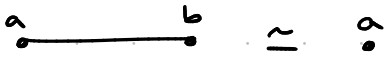
\includegraphics[width=0.25\textwidth]{18_905-201207-1.png}
\end{center}

On the other hand, if we have two objects with two paths between them,
i.e.\ they are equal in two different ways.
In particular, there are two different equalities between them.
We can use one path to identify them,
but then we have the other equality left.
This is the same as a single object with a nontrivial automorphism.
\begin{center}
  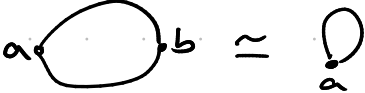
\includegraphics[width=0.25\textwidth]{18_905-201207-2.png}
\end{center}

Similarly, if we have an extra object
  \(c\) that is uniquely identified with \(b\),
  then we identify \(b\) and \(c\),
  and then it reduces to the previous case.
\begin{center}
  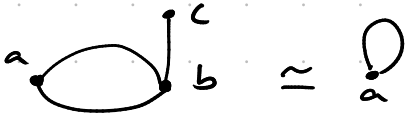
\includegraphics[width=0.25\textwidth]{18_905-201207-3.png}
\end{center}

Note that these are just homotopy equivalences of graphs.
In the spirit of higher category theory,
we can also think about equalities between equalities.
\begin{center}
  
\includegraphics[width=0.25\textwidth]{18_905-201207-4.png}
\end{center}
This is equivalent to saying \(D^2 \simeq *\).

In general, homotopy theory is about objects, equalities between objects,
\(2\)-equalities between equalities, etc.


\section{Algebraic topology}
One example of a question we ask in algebraic topology is:
``Can we classify all \(n\)-dimensional compact manifolds up to homomorphism?
  What about smooth manifolds up to diffeomorphism?''

For example, surfaces (\(2\)-dimensional compact manifolds) are classified.
For example, \(\ZZ\)-oriented surfaces are classified by their genus.
In particular, it is determined by its first homology group.

However, when we increase the dimension, the manifolds get very complicated,
so we can ask the question about manifolds with particularly simple homology.
\begin{theorem}[Kervaire-Milnor, 1961]
  Classification of all compact simply connect \(n\)-dimensional
  manifolds \(M\) with
  \[
    H^q(M) \iso \begin{cases*}
      \ZZ & if \(q = 0, n\) \\[-1ex]
      0 & otherwise
    \end{cases*}
  \]
  for \(n \geq 5\).
  For lower dimensions, we have known \(n = 2\) since around 1900,
  we know \(n = 3\) due to Perelman in 2003, and \(n = 4\) is still unknown.
\end{theorem}

We can also ask if we can classify simply connected and compact
\(2n\)-dimensional manifolds \(M\) where \(H_0(M) \iso \ZZ\) and
\[
  H_1(M) \iso H_2(M) \iso \dots \iso H_{n - 1}(M) \iso 0.
\]
Every simply connected space is \(\ZZ\)-orientable, so it follows that
\[
  H_{n+1}(M) \iso H_{n+2}(M) \iso \dots \iso H_{2n}(M) \iso \ZZ.
\]
\(H_n(M)\) can be anything.
This is classified in all dimensions \(2n\) except \(2n = 4, 24, 126\).

\begin{itemize}
  \item \(n \equiv 6 \mod 8\) was proved by Wall in 1962
  \item \(n \equiv 5 \mod 8\) was proved by Brown and Peterson in 1966
  \item \(n \equiv 3 \mod 8\) was proved by Browder in 1969
  \item \(n \equiv 2 \mod 8\) was proved by Schultz in 1972
  \item \(n \equiv 1 \mod 8\) was proved by Stolz in 1985
  \item \(n \equiv 7 \mod 8\) and \(n \neq 63\) was done by
        Hill-Hopkins-Ravenel in 2009.
        At the time it was proved, Hopkins was a professor at MIT and
        Hill was a graduate student at MIT. % chktex 13
        He is now at UCLA and is the head of
        the LGBTQ society of mathematicians.
  \item \(n \equiv 0 \mod 4\) and \(n \neq 12\) was done by
        Burkland-Senger-Hahn in 2019. Burkland and Senger are
        grad students at MIT, and Hahn is the lecturer of this course!
        Adela Zhang is thinking about extending this to when
        two homology groups are nonzero.
\end{itemize}


\section{More homotopy theory}
\begin{question}
  If \(m\) and \(n\) are positive integers,
  how many maps are there from \(S^m \to S^n\) up to homotopy?
  The set of maps \(S^m \to S^n\) up to homotopy is denoted \(\pi_m S^n\).
\end{question}

On the homework, we proved \(\pi_3 S^2\) has more than one element.
In 18.906, we will see that
\begin{enumerate}
  \item If \(m < n\), all maps \(S^m \to S^n\) are homotopic,
        i.e.\ \(\pi_m S^n\) has one element.
  \item If \(m = n\), then \(\pi_m S^m \iso \ZZ\).
        Maps \(S^m \to S^m\) are determined up to homotopy by their degrees.
  \item If \(m > n\), then unless \(m = 2n - 1\), \(\pi_m S^n\) is finite.
\end{enumerate}
A natural question to ask is how large is this set?
Moreover, note that \(\pi_m S^n\) is not just a set,
but a group in the following way:
If we have two maps \(f, g \colon S^n \to S^n\),
we first ensure (by homotopy) that the south pole of \(f\)
is mapped to the same point as the north pole of \(g\).
Then, \(f * g\) is the map depicted in the following diagram,
where we first pinch the equator,
and then we map the top half by \(f\) and the bottom half by \(g\).
\begin{center}
  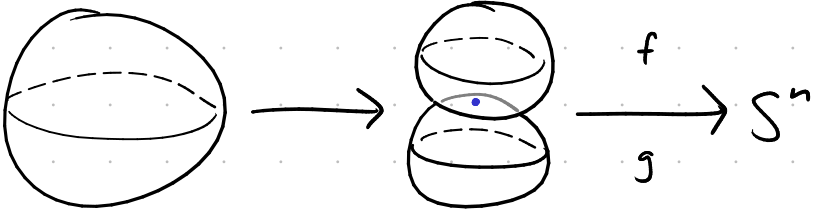
\includegraphics[width=0.5\textwidth]{18_905-201207-5.png}
\end{center}








\end{document}

\documentclass{standalone}
\usepackage{chez}

\begin{document}
\chapter{December 09, 2020}

\section{Homotopy groups of spheres}
Recall that \(\pi_m S^n\) is the group of continuous maps
from \(S^m\) to \(S^n\) up to homotopy.

\begin{theorem}[Freudenthal]
  For \(n \geq k + 2\), \(\pi_{n+k} S^n\) is independent of \(n\).
  This group is denoted \(\pi_k \mathbb S\).
\end{theorem}
\begin{example}
  \(\pi_3 S^2 \iso \ZZ\),
  \(\pi_4 S^3 \iso \ZZ/2\ZZ\),
  \(\pi_5 S^4 \iso \ZZ/2\ZZ\), \dots,
  so \(\pi_1 \mathbb S \iso \ZZ/2\ZZ\).
\end{example}

The first couple of stable groups are
\begin{itemize}[nosep]
  \item \(\pi_1 \mathbb S \iso \ZZ/2\ZZ\)
  \item \(\pi_2 \mathbb S \iso \ZZ/2\ZZ\)
  \item \(\pi_3 \mathbb S \iso \ZZ/8\ZZ \oplus \ZZ/3\ZZ\)
  \item \(\pi_4 \mathbb S \iso 0\)
  \item \(\pi_5 \mathbb S \iso 0\)
  \item \(\pi_6 \mathbb S \iso \ZZ/2\ZZ\)
  \item \(\pi_7 \mathbb S \iso \ZZ/16\ZZ \oplus \ZZ/3\ZZ \oplus \ZZ/5\ZZ\)
  \item \(\pi_8 \mathbb S \iso \ZZ/2\ZZ \oplus \ZZ/2\ZZ\)
\end{itemize}

\begin{question}
  How can we use homology to understand these groups?
\end{question}
An element of \(\pi_7 \mathbb S^n\) is a map
\[
  f \colon S^{7 + n} \to S^n
\]
for \(n \gg 0\).
Then \(H_*(f) \colon H_*(S^{7+n}) \to H_*(S^n)\) is going to trivial
no matter what \(f\) is.

\begin{definition}
  A map of spheres \(S^m \to S^n\) has \vocab{\(\FF_p\)-Adams filtration}
  at least \(k\) if it can be factored as a composite
  \[
    \begin{tikzcd}
    	S^m \ar[r, "f_1"] &
    		X_1 \ar[r, "f_2"] &
    		X_2 \ar[r, "f_3"] &
    		X_3 \ar[r, "f_4"] &
    		\cdots \ar[r, "f_k"] &
    		X_k = S^n
    \end{tikzcd}
  \]
  such that each \(H_*(f_i; \FF_p)\) is trivial.
\end{definition}
Intuitively, this means that it is hard to figure out what is going on
when viewed through homology, because we can factor the map
but still don't understand what the individual maps are.

One way that we can think about it graphically is
with a table like the following
\begin{tcolorbox}[sidebyside, blanker, halign=center, halign lower=center]
  \begin{tikzpicture}
    \matrix (T) [matrix of nodes,
                 nodes in empty cells,
                 matrix anchor=south west,
                 nodes={minimum size=14},
                 row sep=0,
                 column sep=4pt] {
      8 &&&&&&&& \\7 &&&&&&&& \\ 6 &&&&&&&& \\ 5 &&&&&&&& \\ 4 &&&&&&&& \\
      3 &&&&&&&& \\ 2 &&&&&&&& \\ 1 &&&&&&&& \\ 0 &&&&&&&& \\
      & 1 & 2 & 3 & 4 & 5 & 6 & 7 & 8 \\
    };
    \node[rotate=90, yshift=4] at (T.west) {Adams filtration};
    \node                       at (T.south) {Degree \(k\)};
    \draw (T-1-1.north east) -- (T-10-1.south east);
    \draw[transform canvas={yshift=2}]
          (T-10-1.north west) -- (T-10-9.east |- T-10-1.north);

    \begin{scope}[gray]
      \foreach \row in {1,...,8}{
        \draw[transform canvas={yshift=1.2}]
              (T-\row-2.south west) -- (T-\row-9.south east);
      }
      \foreach \col in {2,...,8}{
        \draw[transform canvas={xshift=1.8, yshift=2}]
             (T-1-\col.north east) -- (T-9-\col.south east);
      }
    \end{scope}
    \begin{scope}[transform canvas={yshift=2}]
      \foreach \row / \col in {8/2, 7/3, 6/4, 7/4, 8/4, 7/7,
                               5/8, 6/8, 7/8, 8/8, 6/9, 7/9}{
        \fill (T-\row-\col) circle (1.8pt);
      }
      \begin{scope}[line width=0.6]
        \draw (T-6-4.center) -- (T-8-4.center);
        \draw (T-5-8.center) -- (T-8-8.center);
      \end{scope}
    \end{scope}
  \end{tikzpicture}
  \tcblower
  \begin{itemize}
    \item \(\pi_1 \mathbb S_{(2)} = \ZZ/2\ZZ\)
    \item \(\pi_2 \mathbb S_{(2)} = \ZZ/2\ZZ\)
    \item \(\pi_3 \mathbb S_{(2)} = \ZZ/8\ZZ\)
    \item \(\pi_4 \mathbb S_{(2)} = 0\)
    \item \(\pi_5 \mathbb S_{(2)} = 0\)
    \item \(\pi_6 \mathbb S_{(2)} = \ZZ/2\ZZ\)
    \item \(\pi_7 \mathbb S_{(2)} = \ZZ/16\ZZ\)
    \item \(\pi_8 \mathbb S_{(2)} = \ZZ/2\ZZ \oplus \ZZ/2\ZZ\)
  \end{itemize}
\end{tcolorbox}
Here, we're localizing at the prime \(2\).
In particular, since \(\pi_3 \mathbb S = \ZZ/8\ZZ \oplus \ZZ/3\ZZ\),
we have \(\pi_3 \mathbb S_{(2)} \iso \ZZ/8\ZZ\).
To read the table, we look at each column individually.
The number of dots tells us what the group is,
and the connections tell us how large the powers of the primes are.
The placement of the first dot tells us what the Adams filtration is.
For instance, for degree \(3\), we can interpret the table as saying that
\(\frac{1}{2}\) of the elements in the homotopy groups are
in Adams filtration \(1\),
\(\frac{1}{4}\) of the elements are in Adams filtration \(2\), and
\(\frac{1}{8}\) of the elements are in Adams filtration \(3\).

When we extend the chart, we start to become limited due to computation power.
Ten years ago, we were able to compute the chart
up to around degree \(\sim 50\), and now we have the chart up to degree \(96\).
This chart is on page 8 of \verb|Adamschart.pdf|.

\begin{center}
  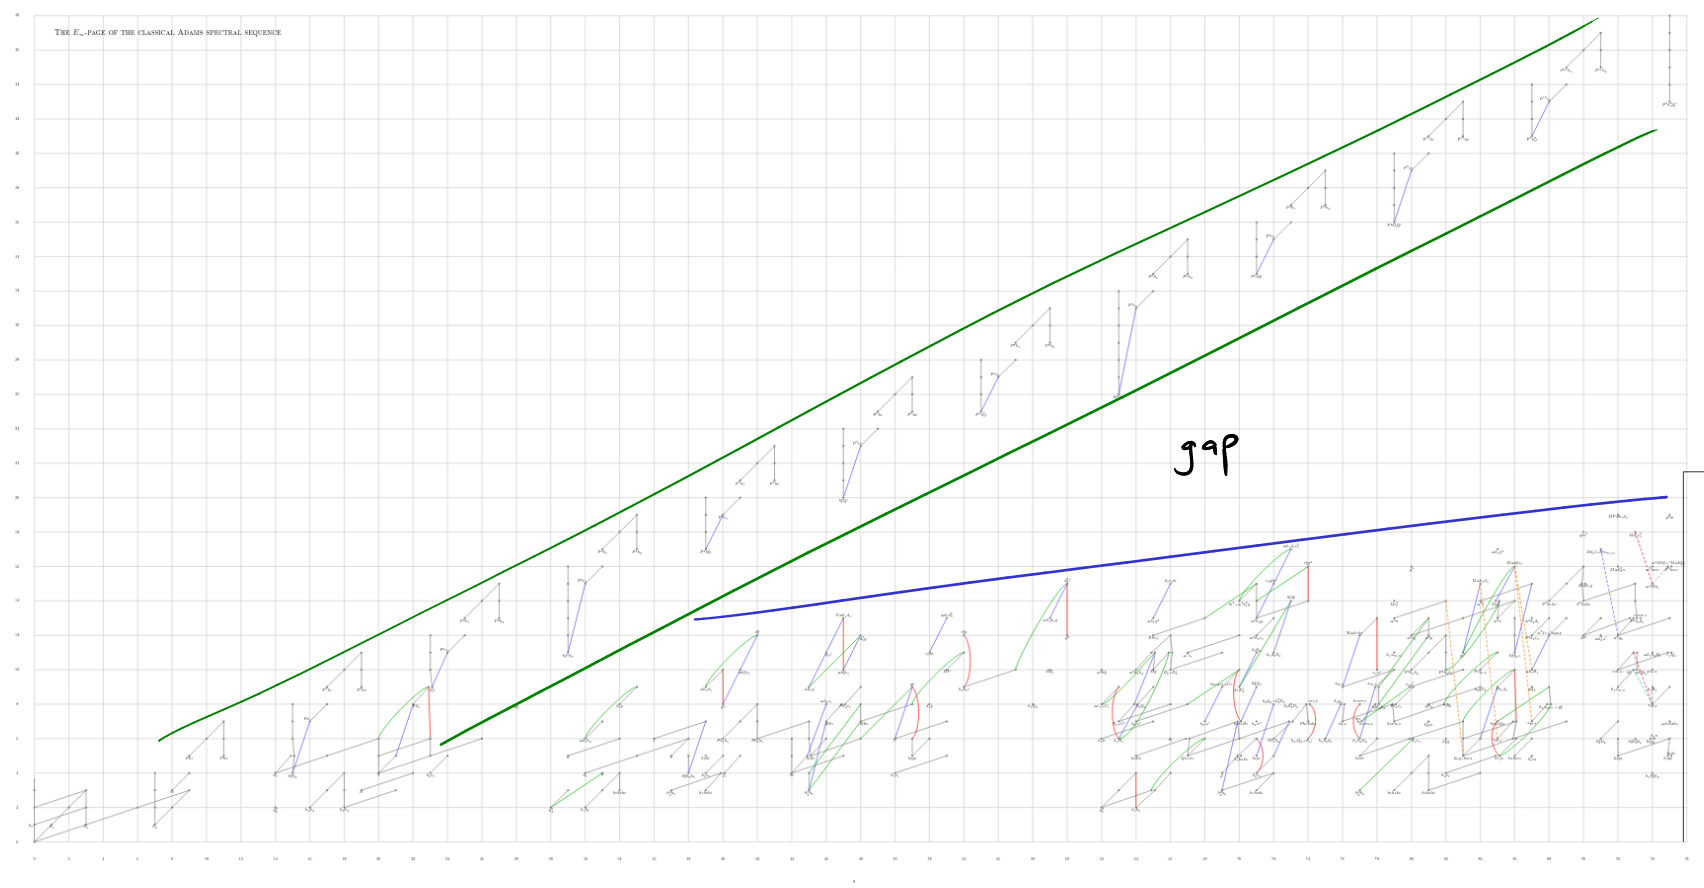
\includegraphics[width=\textwidth]{18_905-201207-6.png}
\end{center}

When we look at the chart, we see that there is a simple collection
of points with larger slope than the rest of the points, indicated with green.
There is also a chaotic pattern of points below it, with a gap in between.

In particular, there are a simple group of homotopy groups
that are hard to detect with homology,
and then there is a messy collection of homotopy groups that
are easier to detect (but still quite hard) with homology.

There is indeed a good understanding of the maps corresponding to
very high Adams filtration, and this region is called
the \(v_1\)-periodic homotopy groups of spheres.
Then there seems to be a gap, and an open problem is
whether this gap continues, and how big it is.
Another natural question is whether we can understand the
non-\(v_1\)-periodic stuff.


\begin{definition}
  An \vocab{extraordinary (co)homology theory} \(E_*\) is a functor % chktex 36
  \[
    E_* \colon \cHoTop \to \text{graded \(\cAb\) groups}
  \]
  satisfying all of the Eilenberg-Steenrod axioms except the dimension axiom.
\end{definition}

They can directly tell, sometimes,
the differences between various maps \(f \colon S^m \to S^n\).
In particular, \(E_*(f) \colon E_*(S^m) \to E_*(S^n)\) could be nontrivial,
because the homologies of a sphere do not have to be
concentrated in one degree.

The most important example is \(E_* = KO_*\),
called \vocab{topological \(K\)-theory}.
This theory sees the \(v_1\)-periodic part of \(\pi_* \mathbb S\).
It has a geometric definition in terms of vector bundles,
which assemble to define \(K\)-theory.
It also has a more algebraic/combinatorial definition.

\begin{question}
  How do we make extraordinary (co)homology theories that detect % chktex 36
  other elements in \(\pi_* \mathbb S\)?
\end{question}

\begin{definition}[Idea]
  An \vocab{\(\mathbb E_\infty\)-ring} is a cohomology theory \(E^*\)
  valued in graded commutative rings.
\end{definition}

For example, we could have \(E^*(X) = H^*(X; R)\),
  where \(R\) is a commutative ring.
We can also have \(E^*(X) = KO^*(X)\).

Given an \(\mathbb E_\infty\)-ring \(E^*\),
we can extract a classical ring, which is \(E^*(*)\).
For example, the classical ring underlying \(H^*({-}; R)\) is
  \(H^*(*; R) \iso R\) in degree \(0\).
On the other hand, the classical ring underlying \(KO^*({-})\) is
  \(KO^*(*)\), which is \(8\)-periodic. (Bott peridicity)

The main idea of algebraic homotopy theory is that we should develop
all of commutative algebra replacing rings with \(\mathbb E_\infty\)-rings.
In particular, wherever we have concepts about rings
like PIDs or Nakayama's lemma, we should try to find an analogous theorem
about \(\mathbb E_\infty\)-rings.
This is what Waldhausen called ``brave new algebra'',
which is today sometimes called ``higher algebra'',
                                ``spectral algebra'', or
                                ``derived algebra''.
A lot of the results we get are the same, but sometimes there are difference.

\begin{example}
  In classical algebra or number theory, people study elliptic curves.
  To imitate the theory of elliptic curves in \(\mathbb E_\infty\)-rings,
  we are led to the notion of \vocab{elliptic cohomology theories}.
\end{example}

One intersecting thing that doesn't happen in classical number theory is that
there is a universal elliptic cohomology theory.
In particular, there is an elliptic cohomology theory that captures the
information of all other elliptic cohomology theories.
This is a new phenomenon that we cannot understand with regular rings.
This universal theory is called \vocab{topological modular forms} (tmf).

We can try to understand the underlying classical ring by
looking at the underlying classical ring \(\mathrm{tmf}^*(*) \otimes_\ZZ \QQ\),
and it turns out to be the classical ring of modular forms.

One can keep going into things like automorphic forms or abelian varieties
and try to construct analogs in this land of brave new algebra.
\(\mathbb E_\infty\)-rings are about commutative algebra,
but we can also talk about associative rings,
which are called \(\mathbb E_1\)- rings.
When we do this, we get a lot of analogs,
and oftentimes we get more objects that we can construct
compared to classical ring theory,
and a lot of the time they are universal.
This is the topic of study in \vocab{chromatic homotopy theory},
which assembles the homotopy groups \(\pi_* \mathbb S\) out of things
detected by \(\mathbb E_\infty\)-rings.
Each \(\mathbb E_\infty\)-ring has a chromatic height that roughly measures
how much of the homotopy group it can see.
\begin{itemize}[nosep]
  \item Height 0 is ordinary homology,
  \item Height 1 is topological \(K\)-theory,
  \item Height 2 is TMF, and so on.
\end{itemize}
Furthermore, we have the chromatic convergence theorem, which says that
each element in \(\pi_* \mathbb S\) is detected at some chromatic height.

Another big open question in this subject is whether
there is a geometric construction of TMF. % chktex 13
For example, we can understand ordinary homology through cycles and
maps of simplices, and we can understand \(K\)-theory with vector bundles.
Physicists tell us that it should be related to the Dirac operator
on the space of loops in \(X\).
However, nobody has been able to do this mathematically in a well defined way.









\end{document}

% insert here



\end{document}
